\documentclass[11pt]{report} %% 12pt Norberts Vorlage
\usepackage[T1]{fontenc}
\usepackage[utf8]{inputenc}

%\usepackage{showframe}
\usepackage{% 
	ae,
	array,
	newtxtext,  %% hier kann man die Schriftart einstellen
	graphicx,
	url,
	units,
	pgfplotstable,
	color,
	colortbl,
	pgfplots,
	cleveref,
	float,
	lipsum,
	textcomp,
	hyperref,
	gensymb,	
	amsmath,
	hyphenat,	 	 
	mathtools,
	mathrsfs,
	physics,
	import,
	amssymb}
	\usepackage[german,british]{babel}
	\usepackage[straightlabels, american, europeanvoltages]{circuitikz}
	\usepackage[a4paper, total={16cm, 24cm}]{geometry} % Reduce margin size from 0.7*paper size
	\usepackage[titletoc]{appendix}
	\usepackage[margin=0.5cm]{caption}
	\usepackage[allow-number-unit-breaks]{siunitx}

%%%%%%%%%%%%% CUSTOM COMMANDS %%%%%%%%%%%%%%
%\newcommand{\tightoverset}[2]{\mathop{#2}\limits^{\vbox to -.5ex{\kern-0.75ex\hbox{$#1$}\vss}}}
\renewcommand{\epsilon}{\varepsilon}
\renewcommand{\vec}[1]{\mathbf{#1}}
\newcommand{\mat}[1]{\underline{\mathbf{#1}}}
\newcommand{\st}[1]{$_{\text{#1}}$}
\newcommand{\er}{$\epsilon_r$}
\newcommand{\tand}{$\tangent\delta$}
\newcommand{\te}{TE$_{\text{011}}$}

%%%%%%%%%%%%%% PGF/TIKZ SETUP %%%%%%%%%%%%%%%%
\pgfplotsset{compat=1.13}
\usetikzlibrary{calc, arrows, graphs,decorations.markings}
\usepgfplotslibrary{smithchart, external, units}
%\tikzexternalize

%%%%%%%%%%%%%% OTHERS %%%%%%%%%%%%%%%%%%%%
\sisetup{detect-weight=true, detect-family=true}
\graphicspath{{./figures/}}
\hypersetup{bookmarksnumbered,
			hidelinks,
    		pdfauthor={Max Gattringer},
            pdftitle={An Improved Model for Complex Permittivity Measurements with a Split-Cylinder Resonator},
            pdfsubject={Master thesis about dielectric measurements at microwave frequencies using a split-cylinder resonator},
            pdfkeywords={dielectric properties; printed-circuit boards; substrates, split-cylinder resonator; microwaves; quality factor measurements; permittivity; cylindrical cavity; mode-matching; cavity; loss tangent; dielectric; microwave substrates; complex permittivity; material properties, dielectric measurements},
            pdfproducer={},
            pdfcreator={}
    } % Hyperlinks, PDF Bookmarking

%%%%%%%%%%%%%% UNICODE CHARS %%%%%%%%%%%%%%%%%%%
\DeclareUnicodeCharacter{221E}{$\infty$}
\DeclareUnicodeCharacter{03C3}{$\sigma$}

%%%%%%%%%%%%%%% HYPENATIONS %%%%%%%%%%%%%%%%%%%%
\hyphenation{per-mit-tiv-i-ty}
\hyphenation{Ja-ne-zic}


%%%%%%%%%%%%% DOCUMENT %%%%%%%%%%%%%%%%%%%%%%%%%%%%%%%%%%%%%%%%%%
\begin{document}
%%%%%%%%%%% TITLEPAGE & DEDICATION %%%%%%%%%%
\begin{titlepage}
\pagestyle{empty}
\newgeometry{total={13.5cm, 23.25cm}}
\begin{center}

\vspace*{1cm}


\includegraphics[width=0.40\linewidth]{TULogo.pdf}

\vspace{3cm}

\LARGE

\textbf{An Improved Model for Complex Permittivity Measurements with a Split-Cylinder Resonator}

\vspace{2.5cm}

\Large

\textbf{Max Gattringer, BSc.}

\large

\vspace{4cm}


Thesis submitted to the Technische Universität Wien for the degree of Master of Science in Telecommunications at the Institute of Electrodynamics, Microwave and Circuit Engineering. 

\vspace{1cm}

Supervisors:\\
\Large
Ass.Prof. Dipl.-Ing. Dr.techn. Holger Arthaber\\
Dipl.-Ing. Norbert Leder

                 

\large
\vspace{1.5cm}

April 2017

\vspace{1cm}

Version 1.01
\end{center}
\end{titlepage}
\restoregeometry
\pagestyle{plain}

%%%%%%%%%%% ACKNOWLEDGEMENTS %%%%%%%%%%%%%%%%
\newgeometry{total={13.5cm, 23.25cm}}
\chapter*{Acknowledgements}
\begin{center}

\vspace{3.5cm}

Before we begin, I would like to thank my family - Hans, Eva Maria, Christian and Claudia Gattringer - for their long lasting support for my studies. They have never questioned any of this. This thesis is dedicated to you!

\vspace{1.5cm}
\textbf{*}
\vspace{1.5cm}

Then again, I would not have survived my studies without all my dear friends and colleagues. Thank you so much!

\vspace{1.5cm}
\textbf{*}
\vspace{1.5cm}

Finally, I want to thank Norbert Leder for his help and encouragement as a supervisor of this thesis!

\vspace{1.5cm}
\textbf{\~{}}
\vspace{1.5cm}


\end{center}

\pagebreak
\restoregeometry

%%%%%%%%%%% ABSTRACT %%%%%%%%%%%%%%%%%%%%%%%%
\newgeometry{total={13.5cm, 23.25cm}}
\chapter*{Abstract}
\addcontentsline{toc}{chapter}{Abstract}
The increasing use of microwave signals in consumer electronics has renewed interest in the dielectric properties of materials at microwave frequency bands. The dielectric properties of materials are important parameters in many areas of electronics design, including electromagnetic compatibility, signal integrity, mixed signal circuit, and RF printed-circuit design. Industry and academia therefore require accurate measurement methods for determining the dielectric properties at these frequencies. 

This thesis builds on an existing dielectric measurement method that is widely considered a very important industry standard for dielectric measurements at microwave frequencies, the split-cylinder resonator method, and improves its capabilities and verifies these improvements experimentally. This method determines the dielectric properties of a flat specimen using the TE\st{0np} modes of a resonator, which is formed by the flat specimen and the two halves of a split cylindrical cavity. Previous studies have modelled this resonator as a symmetric resonator with two identical halves. This thesis expands the method by using an asymmetric model instead of the symmetric one. This asymmetric model is supposed to account for geometric imperfections of the two halves, and thereby improve the accuracy of the method. Such geometric imperfections, namely slight asymmetries of the two cavities, are very likely to occur if the two halves of the cylindrical cavity have been made with general purpose tooling. 

This thesis analyses many aspects of the method, including quality factor measurement methods, the coupling of the resonator, and the field configuration of the resonator. Most importantly, it derives a new asymmetric model for the resonator from Janezic's mode-matching model. Since this new asymmetric model cannot be used to calibrate the resonant frequencies and the conductor losses of the resonator, a separate model is derived for that purpose. Furthermore, the convergence of the asymmetric models is studied. These models were also implemented in software to carry out experimental measurements with a custom measurement setup. This setup was equipped with a novel electromechanical coupling adjustment mechanism to facilitate repeatable measurements. Through an uncertainty analysis of dielectric measurements performed with the new model, it is shown that the model can indeed improve the accuracy of dielectric measurements with a split-cylinder resonator. Additionally, the results of four measurement studies with the new model, which include measurements of microwave substrates and plastics, a repeatability evaluation, and measurements with higher modes, are presented.
\pagebreak

\chapter*{Kurzfassung}
\begin{otherlanguage}{german}
Durch die zunehmende Nutzung von Mikrowellen in der Elektronik haben in letzter Zeit die dielektrischen Eigenschaften von Werkstoffen bei diesen Frequenzen immer mehr an Bedeutung gewonnen. Grund hierfür ist die große Bedeutung dieser Eigenschaften für viele Teilgebiete der Elektronik\-entwicklung, wie der Vermeidung von elektromagnetischen Störungen, der Sicherung der Signal\-integrität sowie des Entwurfs von Hoch\-fre\-quenz\-schalt\-ungen und Mixed-\-Signal-\-Schaltungen.

Diese Diplomarbeit beschäftigt sich mit einer dielektrischen Messmethode, der Split-\-cylinder Resonator Methode, die auch ein bedeutender Industriestandard für die Bestimmung der dielektrischen Eigenschaften bei Mikrowellenfrequenzen ist. Diese Arbeit baut hierbei auf früheren wissenschaftlichen Abhandlungen zu dieser Messmethode auf, verbessert sie aber verglichen zu diesen und verifiziert diese Verbesserungen experimentell. Die dielektrischen Eigenschaften von dünnen Dielektrika lassen sich mit dieser Methode unter Verwendungen der TE\st{0np}-Moden eines Resonators bestimmen, der aus dem dünnen Dielektrikum und aus den zwei Hälften eines in der Mitte geteilten kreiszylindrischen Hohlraumresonators gebildet wird. In früheren Abhandlungen wurde dieser Resonator immer mit einem symmetrischen Modell mit zwei identen Hohl\-raum\-resonator\-hälften beschrieben. In dieser Arbeit jedoch wird die Methode erweitert, indem anstatt dieses symmetrischen Modells ein asymmetrisches verwendet wird. Die Aufgabe dieses asymmetrischen Modells ist dabei Größen\-unterschiede zwischen diesen Hohl\-raum\-resonator\-hälften in das Modell einzubeziehen um hierdurch die Genauigkeit der Messmethode zu verhöhen. Solche Größen\-unterschiede treten sehr häufig auf, wenn zur Fertigung der Hohlraum\-resonatoren Standardwerkzeug hergenommen wurde.

Im Rahmen dieser Arbeit werden verschiedene Teilaspekte dieser Messmethode untersucht, unter anderem Methoden zur Bestimmung der Güte, die Kopplung des Resonators und die Feldverteilung im Resonator. In erster Linie wird aber ein neues, asymmetrisches Modell hergeleitet, das von Janezics Mode-Matching Modell abgeleitet wurde. Da ein asymmetrische Modell des gesamten Resonators nicht direkt zu Kalibrierung der Resonanzfrequenzen und der Leiterverluste des Resonators eingesetzt werden kann, wird zusätzlich noch ein Kalibrierungs\-modell hergeleitet. Darüber hinaus wird die Konvergenz beider Modelle überprüft. Für Versuchsmessungen mit einem selbstentwickelten Messaufbau wurden diese Modelle in Software implementiert. Um die Wiederholbarkeit der Messungen mit diesem Messaufbau zu verbessern, wurde der Messaufbau zusätzlich mit einem neuartigen elektro-mechanischen Kopp\-lungs\-anpass\-ungs\-mech\-an\-is\-mus ausgestattet. Mittels einer Fehleranalyse von dielektrischen Messungen mit dem neuen Modell wird gezeigt, dass das Model wirklich die Genauigkeit der dielektrischen Messungen mit dem Resonator erhöhen kann. Zusätzlich zu dieser Fehleranalyse, werden auch die Ergebnisse von vier Versuchsmessungen vorgestellt, in denen verschiedene Mikrowellen\-substrate und Kunststoffe gemessen werden, die Wiederholpräzision der Methode abgeschätzt wird und auch Messungen mit höheren Moden untersucht werden.
\end{otherlanguage}
\pagebreak
\restoregeometry


%%%%%%%%%%%%%%%%%%%%%%%%%%%%%%%%%%%%%%%%%%%%%%%%%%%%%%%%%%%%%%%%%
\bibliographystyle{IEEEtran}
%%%%%%%%%%%%% TOC %%%%%%%%%%%%%%%%%%%%%%%%%%%%%%%%%%%%%%%%%%%%%%%
\setcounter{tocdepth}{1}
\renewcommand*\contentsname{Table of Contents}
\tableofcontents
\addcontentsline{toc}{chapter}{Table of Contents}
%%%%%%%%%%%%% CHAPTERS %%%%%%%%%%%%%%%%%%%%%%%%%%%%%%%%%%%%%%%%%%
%\input{chapters/introduction} % Introduction
\chapter{Dielectric Measurement Methods at Microwave Frequencies}\label{ch:methods}
\section{Introduction}
The ever increasing bandwidth requirements and the demand for better availability for mobile equipment is constantly pushing wireless communications to higher frequencies and greater efficiencies. Microwave engineering and material sciences have to keep pace with these recent developments. Dielectrics like microwave substrates or dielectric resonators play an important role in their efforts, since integrates circuits, printed circuits, filters and antennas - just to name a few applications - require well-characterised and understood dielectrics that perform well at microwave frequencies. Accurate characterisation of dielectrics is particularly important, as it could enable capabilities in rapid prototyping that have previously been unfeasible.

In the past, characterising dielectrics accurately at microwave frequencies has been relatively expensive and complicated. Out of this reason, both dielectric constant and loss tangent have often eluded measurement by scientists and engineers. While this applied to all dielectrics, it applied even more to low-loss dielectrics, which are often used as microwave substrates in integrated circuits and printed circuits. These materials typically have a very low dielectric loss, which can only be measured accurately with standing-wave methods (also called resonator methods). Unfortunately, many standing wave methods measure the permittivity only at one frequency (the resonant frequency) and very often the specimens have to be machined in order to measure them inside a resonator. The topic of this thesis is a standing-wave method that circumvents these two disadvantages of many standing-wave methods - the split-cylinder resonator method. 

The split-cylinder resonator is a very popular standing-wave dielectric measurement method, which was designed to operate at microwave frequencies. It uses a microwave cavity, which is split into two halves, an upper and a lower cavity. In between these two cavities a flat dielectric specimen can be placed, whose permittivity can then be measured by exciting one or multiple modes in this resonator. The specimen does not have to be prepared in any way before the measurement, as long as the specimen is sufficiently flat. The method itself was developed by Ermert \cite{ermert}, Guillon \cite{guillon}, Kobayashi \cite{kobayashi} and Kent \cite{kent1996}. Later, Janezic \cite{janezic} improved the method both in function and in accuracy. He derived a very efficient mode-matching model of the split-cylinder resonator that was widely adopted in the industry. Today, the measurement method is both an IPC standard \cite{ipcSC} and an IEC standard \cite{iecSC}, and it sold commercially by Keysight.

Still, the method has a few minor disadvantages: First of all, it is a relatively expensive method, because it requires a vector network analyser and a split-cylinder resonator, both of which are expensive. Secondly, the resonant frequencies at which the resonator measures the permittivity change with thickness and dielectric constant of the material. Since this is the working principle of the resonator, this cannot be avoided. This property severely disadvantages the split-cylinder over simple stripline techniques, since the permittivity is not measured at frequency bands of interest (e.g. ISM band \SI{2.4}{\giga\hertz}, \SI{10}{\giga\hertz}), but rather at more or less 'random' frequencies. Looking at these disadvantages, we have come up with the idea to reduce the cost of the method by manufacturing the cavities with widely available manufacturing equipment and use these cost reductions to manufacture a resonator for each specimen that has its first \te{} mode - one of the modes the resonator measures with - at a certain frequency.

Although this sounds like an interesting proposition, the use of widely available manufacturing equipment also reduces the accuracy of the method. The reason for this lies in the fact that the currently available electro-magnetic models for the split-cylinder require a symmetric split-cylinder resonator, so an accurate measurement with a split-cylinder would need two half-cavities of the same size. With a lower manufacturing precision, on the other hand, the lengths and diameters of the half-cavities will vary, which would break the symmetry of the model and reduce the accuracy. To retain the accuracy of the method, we found that it would make sense to expand Janezic's mode-matching model to asymmetric split-cylinder resonators, i.e. resonators with unequal half-cavities. 

This thesis therefore aims at deriving a mode-matching model for asymmetric split-cylinder resonators. Before we start this derivation, we first explore the dielectric measurement methods at microwave frequencies in Chapter \ref{ch:methods}. We compare two types of dielectric measurement methods - travelling-wave methods and standing-wave methods. As this thesis is about a standing-wave method, we also introduce three examples for this type of measurement method. In the next chapter, Chapter \ref{ch:splitc}, we then discuss an important aspect of standing-wave dielectric measurements, quality factor measurements, where we explain the theory of resonances in microwave cavities and look into the different methods of measuring the resonant frequency and quality factor of these resonances. In Chapter \ref{ch:splitc} we then continue by taking a closer look at the split-cylinder resonator. We discuss the split-cylinder resonator's field configuration and coupling networks, and we compare the different electro-magnetic models that have been developed for the split-cylinder resonator. After getting a deeper understanding of the resonator, we can then start deriving our model in Chapter \ref{ch:m12}. We derive the model in two parts: In the first part we derive a model for the measurement of the permittivity and in the second part we derive a separate model for the calibration. After these two parts it is shown that both models converge. Finally, in Chapter \ref{ch:results} we present measurement results of measurements that we performed with our model and with a split-cylinder resonator prototype. We first outline what our measurement setup looked like, then we discuss the results of an uncertainty analysis, in which we compared our model to the Janezic model. Lastly, we also show a few experimental measurements that we performed with the split-cylinder resonator prototype.
\section{Dielectric Properties of Materials at Microwave Frequencies}
As we have already emphasised in the last paragraphs, dielectrics play an important role in microwave engineering. They are used in a wide variety of applications ranging from microwave substrates to electro-magnetic absorbers, both of which use dielectrics with very different properties. When we think of dielectrics, we think of materials with very similar properties. In reality, dielectrics are a very diverse group of materials. Non-linear dielectrics like piezoelectric materials, anisotropic dielectrics like crystals and even magnetic materials like ferrites are all dielectrics, since they all do not (or rather poorly) conduct electricity. When we think of dielectrics we therefore always have to ask ourselves, what kind of dielectric we actually want to measure. Microwave substrates and many other materials in microwave engineering are plastics, ceramics or glasses. These materials can be modelled rather conveniently as linear, homogeneous dielectrics. In terms of the field configuration inside the materials this implies that there is a location-independent, linear relationship between the electric field $\vec{E}$ and the electric flux density $\vec{D}$,
\begin{align*}
&\vec{D}=\underline{\epsilon}\vec{E}\text{,} &\underline{\epsilon}=\epsilon'-j\epsilon''\text{,}
\end{align*}
where $\underline{\epsilon}$ is the complex permittivity. The complex permittivity describes to what degree the electric field can polarise the electric dipoles in a dielectric. In an oscillating electric field, as we all know, this polarisation is dampened by molecular and atomic forces, which cause dielectric loss in the material. The polarisation and the dielectrics loss typically vary with the frequency of the oscillating electric field. Accordingly, the complex permittivity is frequency-dependent, or dispersive
\begin{align*}
\vec{D}(\omega)=\underline{\epsilon}(\omega)\vec{E}(\omega)\text{.}
\end{align*}
The driving force behind the frequency dependency of the permittivity $\underline{\epsilon}$ are the different polarisation mechanisms in a dielectric. At microwave frequencies the only noticeable polarisation mechanisms are the dielectric relaxation (dipole or orientational polarisation) of the material and the low frequency tails of the dielectric resonances at higher frequencies. Out of this reason the permittivity of dielectrics is very predictable at microwave frequencies, which facilitates dielectric measurements at our frequency band of interest. At microwave frequencies, the dielectric constant $\epsilon'$ of linear, homogeneous dielectrics \textbf{always falls} with increasing frequency. The imaginary part of the permittivity $\epsilon''$ on the other hand \textbf{can rise and fall}, but its value can be expected to reach a peak in the frequency range, if the materials is a polar material, or to stay almost constant over most of the frequency range and only increase when it comes to the upper end of the frequency range \cite{NPL}.

We have now derived our basic model for dielectrics at microwave frequencies, which we will use to model dielectric throughout this thesis. Still, we will now discuss a few special cases the reader might find useful. The first special case are \textbf{anisotropic dielectrics}: Materials whose dielectric properties are a function of direction are called anisotropic dielectrics. While strong dielectric anisotropy is usually limited to more exotic materials like crystals, many laminar microwave substrates have a weak anisotropy. With weak anisotropy we mean that the permittivity has different values normal (out-of-plane) and tangential to the surface of the substrate (in-plane). In the case of microwave substrates, the origin of this anisotropy is not the base material, but an inhomogeneity of the substrate. Many microwave substrates are in fact composites, but since their constituent materials are far smaller than the wavelengths at microwave frequencies, they still can be considered homogeneous materials. In production the constituent materials of the composites can be aligned, which can then make the composite anisotropic \cite{dankov, NPL, horn}.

The second special case are low-loss dielectrics, which are characterised by their low dielectric loss. Since real dielectrics have near to zero electric conductivity, the dielectric loss is the dominant loss mechanism in a dielectric. As the Kramers-Kronig relations put the dielectric loss in relationship with the dielectric constant, a low dielectric loss has a strong influence on its dielectric constant. It turns out that materials with a very low dielectric loss have dielectric constants that change only very slowly over frequency. Lynch has derived a simple formula from the Kramers-Kronig relations, which illustrates this property very well:
\begin{align*}
&\frac{\Delta\epsilon'}{\epsilon'}\approx m\tan\delta\log_{10}\left(\frac{f_2}{f_1}\right)  & 1\leq m\leq 2.3
\end{align*}
The formula states that the dielectric constant $\epsilon'$ will change from frequency $f_1$ to a higher frequency $f_2$ proportional to the average dielectric loss $\tan\delta=\frac{\epsilon''}{\epsilon'}$ of the material at these frequencies \cite{NPL}.

As we have already stated, there is a true wealth of different dielectrics that are in use in microwave engineering, we decided to limit ourselves to the second special case, low-loss dielectrics, such as substrates used in printed circuit boards, insulators and dielectric resonators. Corresponding to the many varieties of dielectrics, there are just as many different methods for measuring the complex permittivity. At microwave frequencies (1-\SI{100}{\giga\hertz}) we categorize the dielectric measurement methods into \textbf{travelling wave} methods and \textbf{standing-wave} methods, both of which bear 'wave' in their name reflecting the wave nature of the electromagnetic waves at microwave frequencies.
\section{Travelling-Wave Methods}
Travelling-wave methods use the scattering parameters of a measurement cell to directly determine the dielectric properties of a specimen. Waves are emitted into the measurement cell and the response, in the form of transmitted and reflected waves, is measured. The waves typically travel through a waveguide or through free-space in the measurement cell and interact with the specimen while they pass through. The waves enter the measurement cell through one or multiple ports, which may or may not have the same reference impedance. When the wave meets the specimen in the measurement cell the wave is reflected by the transition from the measurement cell medium into the specimen medium. One part of the wave is reflected at this first boundary, another part can transmit through the boundary and propagate in the medium. Depending on the composition of the measurement cell one or multiple boundaries can exist in a cell, which in turn can cause multiple transmission and reflection events. Using suitable models for the measurement cell, we can derive the properties of the specimen. Typically we would like to determine the permittivity $\underline{\epsilon}=\epsilon'-j\epsilon''$ and the permeability $\underline{\mu}=\mu'-j\mu''$ of the specimen. 

Like the permittivity the permeability depends on the frequency, the orientation of the field in the measurement cell, the temperature and the composition of the specimen. While the temperature and composition of a specimen is typically known and is therefore included in the model, the anisotropy of each property is generally not known. To simplify the matters here the specimens can be assumed to be isotropic. Such simplifications limit the number of different specimen types that can be measured, but the approach is feasible since many technically relevant dielectrics are isotropic. This limits the number of unknowns in the measurement to two complex variables ($\underline{\epsilon}$, $\underline{\mu}$), which can be solved using the results of a transmission and reflection measurement ($S_{11}$, $S_{12}$, $S_{21}$ and $S_{22}$). As a result the permittivity and the permeability of a specimen can be derived simultaneously in a transmission and reflection measurement \cite{NPL, chen}.

The decisive advantage of travelling wave methods over standing wave methods is that the measurement frequency can be chosen freely and is not determined by the measurement cell. This allows us to use travelling-wave methods over a very wide range of frequencies as long as the model that we use in our measurements is valid. Another advantage is simplicity, if we assume for example that we only want to measure non-magnetic dielectrics we can use a complex reflection coefficient measurement to measure the complex permittivity of a non-magnetic specimen over a wide frequency range. The downside of travelling wave methods is that we use the results of our scattering parameter measurements directly. While this allows us to perform broadband measurements, it limits the accuracy that we can achieve using this method. This is not so much a problem when we measure the real part of the complex permittivity, but rather when we try to measure the loss tangent. The magnitude of the loss tangent varies very strongly with the type of dielectric. Medium to high-loss dielectrics can have a loss tangent of above one and low-loss dielectrics can have one of around \num{5e-5}. A wave transmitted through a thin, low-loss specimen is barely attenuated by the specimen. The sensitivity of travelling-wave methods for these low-loss specimens is therefore relatively low, and noise and other loss processes also drive up the uncertainty of this method.
\section{Standing-Wave Methods}
Since travelling-wave methods are not able to measure low-loss specimens accurately, we continue this discussion of dielectric measurement methods with the method that lies in the focus of this thesis - the standing-wave or resonance method. The fundamental idea behind the standing-wave method is that the measurement cell is a microwave resonator, which resonates with the specimen inside the measurement cell. Usually the resonant frequency $f_r$ of the measurement cell determines the dielectric constant of the specimen and the quality factor $Q$ the loss tangent. Unlike the travelling-wave method the standing-wave method only measures the complex permittivity at the resonant frequencies of its resonances, so the results lie at discrete frequencies and are not broadband. Although the method delivers far less frequency points, the results of each measurement can be very accurate if implemented correctly. With this qualitative advantage standing-wave methods are usually the most accurate methods for low-loss materials. The measurement cells can be chosen as such that they provide higher field strengths in the specimen for some measurement modes, which increases the loss in the specimen and therefore also the sensitivity of loss measurements. Still, both measurement methods have their merits: For example, a disadvantage of the standing-wave method is that these methods can usually only handle non-magnetic specimens. This makes it very attractive to use a combination of both methods. A non-resonant method is used to get a general knowledge of the electromagnetic properties over a wide frequency range. A resonant method is used to get accurate measurements at discrete frequencies.

Many different variants of the standing-wave method exist, at lower resonant frequencies microwave cavities are used. Cavities are metallic enclosures around a dielectric field region, which can be used as microwave resonators. If the specimen itself is cut to a certain shape and excited by a suitable coupling network, the measurement setup becomes a dielectric resonator. This dielectric resonator can then be used for dielectric measurement, for example for dielectric bricks used in dielectric resonators. At millimetre wave frequencies quasi-optical techniques are used more often, since cavities at these frequencies become increasingly small. All techniques have in common that they require accurate modelling of the measurement cell to compute the complex permittivity from a measured resonance. Many methods use analytical or numerical models of the resonator and the specimen to achieve this. Another approach is the resonant perturbation technique, which has been very popular before the advent of computer-aided electro-magnetics. Resonant perturbation typically means that a small specimen is inserted into a cavity with very well known field configuration inside it. The fields are disturbed by the specimen, but the influence of the specimen is so weak that the field configuration of the cavity without the specimen is altered only slightly. In such case the original solution for the cavity can be used with a simple perturbation term to measure the permittivity of the specimen.

We are now going to introduce three different standing-wave methods. Firstly, we will introduce the planar circuit methods, which are especially popular among printed circuit board manufacturers and circuit designers. We will explain why these methods are usually not the best choice for low-loss specimens and why other methods are usually superior in performance compared to these methods. Secondly, we give a brief introduction into the split-post dielectric resonator, which is one of the most accurate methods for low-loss dielectrics in the 1-\SI{10}{\giga\hertz} frequency range. It is also very similar to the method that is the topic this thesis, the split-cylinder resonator, which we will discuss in Chapter \ref{ch:splitc}. Lastly, we will introduce a microwave Fabry-Perot resonator, the open-resonator method, to give the reader an insight into how dielectric measurements are performed at millimetre-wave frequencies.

\section{Planar Circuit Methods}
\begin{figure}
\centering
\begin{tikzpicture}
%\draw[step=1cm,gray,very thin] (-3,0) grid (13,7.5);
    \node[anchor=south west,inner sep=0] (image) at (0,0) {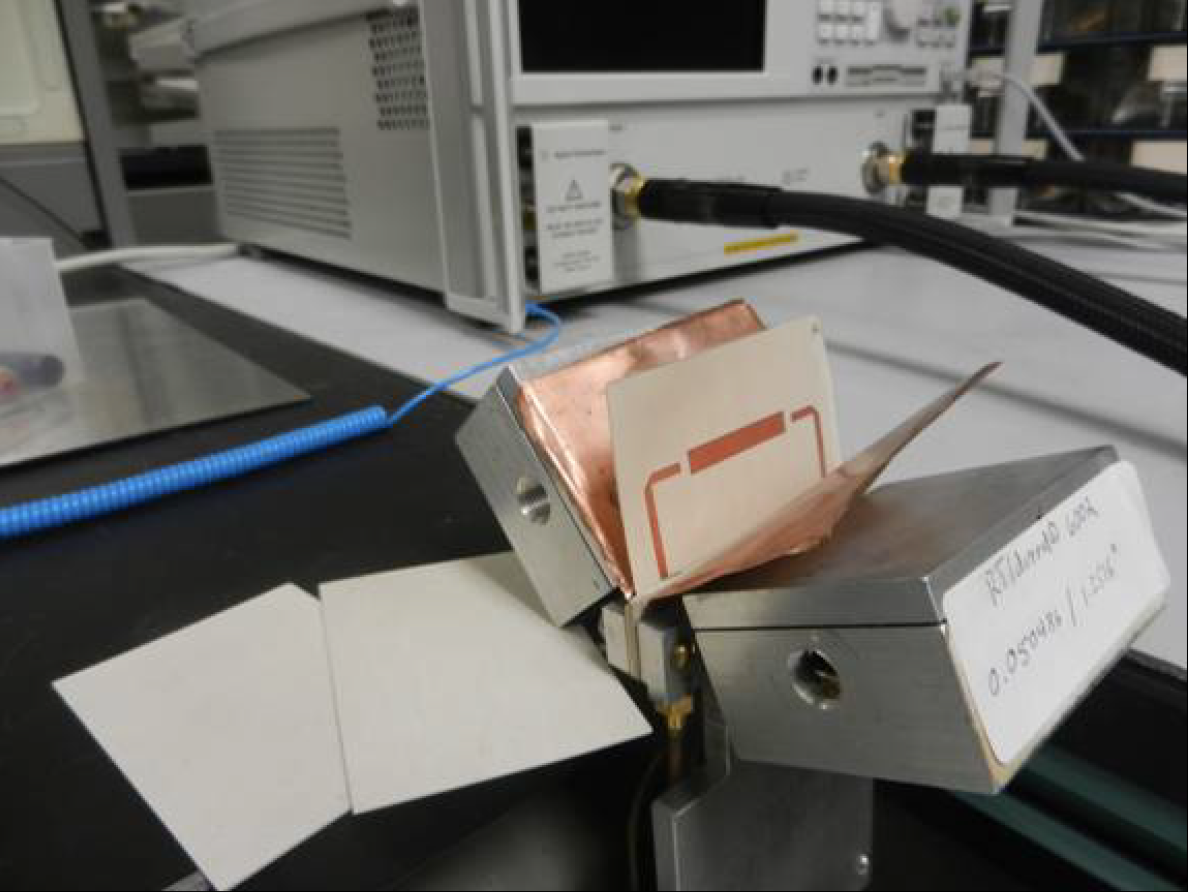
\includegraphics[width=10cm]{figures/tm2555c.png}};
    \draw [-latex, thick, green] (-0.75,6) node[anchor=east, black] {\small Clamp} to (4.5,3.5);
    \draw [-latex, thick, green] (-0.20,4) node[anchor=east, black] {\small Coupling strips} to (5.5,3);
    \draw [-latex, thick, green] (-0.5,2) node[anchor=east, black] {\small Specimens} to (0.5,1.8);
    \draw [-latex, thick, green] (10.75,6) node[anchor=west, black, text width=2cm] {\small Pattern card} to (6.5,4.5);
    \draw [-latex, thick, green] (10.3,4) node[anchor=west, black] {\small Copper sheets} to (7.5,3.75);
    \draw [-latex, thick, green] (10.75,1.5) node[anchor=west, black,text width=2cm] {\small Strip line resonator} to (6,3.75);
\end{tikzpicture}
\caption{Stripline resonator according to IPC TM-650 2.5.5.5c, adapted from \cite{horn}.}\label{fig:tm2555}
\end{figure}

Substrate and printed circuit board manufacturers often perform dielectric measurements, which are very important for the quality control in printed circuit board manufacturing and for the design of electronic circuits. The reason for this is that high-frequency electronics manufacturers need a consistent $\epsilon_r$ value for their production, which implies a tight $\epsilon_r$ control in PCB production. Horn \cite{horn} claimed that the $\epsilon_r$ of a substrate must not vary more than 0.5\% from batch-to-batch and within the sheet itself in order to meet customer requirements. He suggested that a measurement method with an relative accuracy for the $\epsilon_r$ of less than 0.5\% must chosen to measure these small variations in the dielectric substrates. As manufacturers are well experienced with printed circuit techniques, many of them use printed circuits for their dielectric measurement. Typically, they use one of the popular planar transmission lines like striplines, microstrips or co-planar transmission lines. These can be used in travelling-wave methods or standing-wave methods for planar circuits, but we will only discuss the standing-wave methods here as the former suffer from the same issues as other travelling-wave methods. Widely used standing-wave techniques are ring-resonators, T-resonator and strip\-line resonators. Especially the clamped stripline resonator of IPC standard IPC-TM-650 2.5.5.5c \cite{tm650} is widely used by PCB manufacturers and measurement results can be found in many datasheets. The method is illustrated in Fig. \ref{fig:tm2555}, two pieces of unclad substrate are sandwiched together with a thin strip of copper and two coupling strips in the middle, and are then pressed together by two pieces of copper at the top and the bottom. The result is a capacitively coupled strip line resonator, which allows quick and repeatable dielectric measurements that are excellent for quality control.

Planar circuit techniques have very genuine advantages, first of all the field orientation of the electric field in the substrate is the same as in a practical circuit. As single-ended planar transmission lines have one or multiple ground planes, the field orientation in the material is mostly perpendicular to the surface of the material. Combined with the fact that most PCB materials are weakly anisotropic, a measurement method that has the same field orientation as a circuit delivers the right dielectric constant for that circuit. Secondly, planar substrate techniques can include all loss mechanisms in a circuit - dielectric losses and conductor losses. As there are various types of copper claddings available on the market, measuring both loss mechanisms can deliver better predictions for the performance of a circuit as the entire system of copper cladding and dielectric is measured and not only the dielectric. For a PCB manufacturer these two are very important advantages, but these advantages pose serious challenges for dielectric measurements. In case of the field orientation, the orientation of planar circuits is not only perpendicular to the substrate, but there are also fringing fields that have field components parallel to the surface. The influence of fringing fields depends on the type of transmission line. Microstrips, for example, have far stronger fringing fields than strip lines, which can cause measurement errors in anisotropic materials. This makes microstrip resonators and transmission lines far less suitable for dielectric measurements. Another disadvantage of the perpendicular field orientation are potential systematic measurement errors that can be caused by air gaps, which can make a measurement method understate the dielectric constants of high-$\epsilon_r$ laminates.

For the loss measurements the situation is not much better, if we wanted to measure the dielectric losses of a material, we would have to separate the dielectric losses from the total losses in the material. As the conductor losses are typically far higher, there is a large uncertainty for the dielectric losses in the material. This makes substrate methods far less attractive for low-loss dielectrics. For example, according to NIST Technical Note 1520 \cite{tn1520} the ring-resonator and the T-resonator are limited to materials with a loss tangent $\tan\delta>\num{1e-3}$. Additionally the results of open structures like microstrip lines or co-planar strip lines may be affected by radiation losses. Impurities introduced by the manufacturing of the copper cladding may also change the dielectric properties. All in all, planar circuit methods are interesting options for approximate dielectric measurements of cladded printed circuit board substrates, since they offer the right field orientation in the substrate and they include most loss mechanisms in the material. For accurate dielectric measurements they should be used with utmost care, since systematic errors like airgaps, field orientation, anisotropy and conductor losses can negatively affect a measurement.
\section{Split-Post Dielectric Resonator Method}
\begin{figure}
\centering
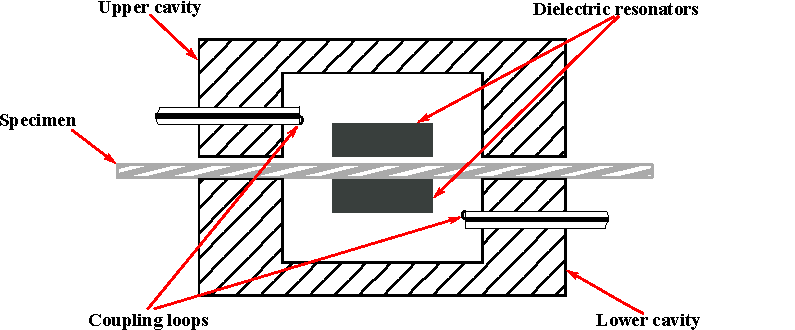
\includegraphics[width=0.8\textwidth]{split_post_dielectric_resonator.pdf}
\caption{Split-post dielectric resonator.}\label{fig:split_dr}
\end{figure}

The second standing wave method that we would like to discuss here, the split-post dielectric resonator method, bears many similarities to the split-cylinder method and other TE\st{0n} mode cavities. It was developed by Krupka, Nishikawa and DelaBalle \cite{dellaballe,nishikawa,krupka} in the 1980s and is one of the easiest and most convenient methods for measuring dielectric properties. It has become an industry standard for the measurement of PCB laminates and dielectric substrate \cite{iecSPDR}. Figure \ref{fig:split_dr} illustrates the geometry of a split-post dielectric resonator. The resonator consists of two cylindrical microwave cavities that both have a dielectric resonator placed along the z-axis of the cavity. One half is placed above the other with a small gap still separating the two halves. The resonator is then excited by coupling loops inserted into the bottom cavity and the top cavity. When the resonator is excited, the two dielectric bricks in the cavity experience a coupled TE\st{01$\delta$} resonance and the two resonators are coupled by evanescent fields. Unlike the evanescent fields of a single resonator, the evanescent fields between the two dielectric resonators are relatively strong. Dielectric specimens can therefore be placed in the gap between the two cavities and perturb the resonance of the resonator. Again, we can use the perturbation of the resonator to measure the complex permittivity of the specimen \cite{NPL, janezicSPDR, krupka}.

Since most of the electro-magnetic energy is stored in the dielectric resonators and in the region between the two resonators, there is far less interaction with the cavity walls than in a typical cavity method. This allows the split-post dielectric resonator to have a far greater sensitivity for dielectric loss measurements and resolutions as low as \num{2e-5} for $\tan\delta$ may be achieved. Split-posts dielectric resonators can be manufactured in a frequency range from \SIrange{1}{36}{\giga\hertz}, but they only operate at a single frequency. Their advantage over other cavity methods is that the frequency shifts of Split-post dielectric resonators are generally smaller and that the measurement frequencies for different specimens are roughly the same - a cavity may be detuned by a specimen as much as \SI{3}{\giga\hertz}! Like TE\st{0n} mode cavities, the evanescent field is also circularly polarised and therefore continuous across air-dielectric interfaces. This mitigates the influence of airgaps and allows the operator to measure thin films and coatings \cite{NPL, janezicSPDR, krupka}.

Although the resonator has many advantages, there are a few downsides: First of all, the modelling of the split-post dielectric resonator is far more complicated than other dielectric measurement methods. There are no analytical models, so numerical techniques like mode-matching, finite-difference, finite-element or Rayleigh-Ritz methods must be employed. Although it is very similar to perturbation methods, it cannot be modelled using perturbation methods. Secondly, their are restrictions on the thickness of the specimens. Specimens can only be as thick as to allow strong coupling between the two resonators. At higher frequencies decoupling issues are more likely, so even thinner specimens may be required. Lastly, the technique is not usable at millimetre frequencies and becomes increasingly hard to use above \SI{10}{\giga\hertz}. At these frequencies cavities have to be very small and the thickness of the specimens is very limited, so split-post dielectric resonators are typically used from 1-\SI{10}{\giga\hertz}. Overall, the split-post dielectric resonator method is an excellent method for measuring thin, low-loss dielectrics in the 1-\SI{10}{\giga\hertz} frequency range. The dielectric constant of thin specimens can be measured with an accuracy of less than $\pm 0.3\%$ and the resolution of the loss tangent measurements may be as small as \num{2e-5}, although these figures may be worse for thicker specimens \cite{NPL, janezicSPDR, krupka}.
\section{Open-Resonator Methods}
\begin{figure}
\centering
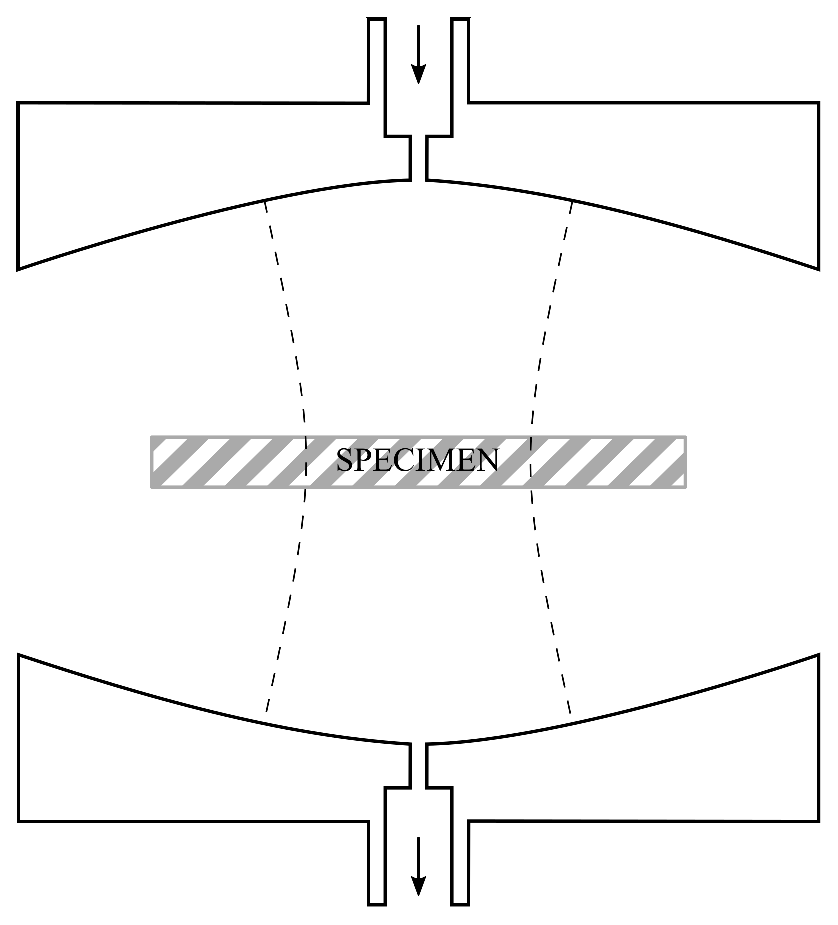
\includegraphics[width=0.4\textwidth]{open_resonator.eps}
\caption{Open resonator with two concave mirrors coupled to waveguides, adapted from \cite{NPL}.}\label{fig:or}
\end{figure}

At millimetre wave frequencies many methods become less practicable. Cavities for example become inconveniently small as their sizes are usually proportional to the wavelength $\lambda$. At these frequencies quasi-optical techniques like the open resonator method are used very often. An open resonator is a microwave Fabry-Perot interferometer, which uses two mirrors to focus electromagnetic waves in between these mirrors. A specimen is then placed between the  mirrors and, like for all other standing wave methods, the quality factor and the resonant frequency of the cavity are used to measure the complex permittivity of a specimen at the resonant frequencies. Different variants of the method exist and they can measure specimens over a wide frequency range 10-\SI{200}{\giga\hertz}. According to NPL \cite{NPL} it is one of the most accurate and important methods for low-loss dielectrics at millimetre-wave frequencies. It allows measuring the dielectric constant with an uncertainty of $\pm 0.2\% $ for $\epsilon_r < 3$, $\pm 1\% $ for $\epsilon_r\approx 50$ and the loss tangent with an uncertainty of $\pm 10\%$ for $\tan\delta >\num{2e-4}$. The measurement modes of the cavity are TEM\st{00n} Gaussian beam modes, so the electromagnetic waves in the cavity are focussed to a beam like in an optical resonator. The field orientation of the electric field varies over the beam length, so the placement of a specimen along the beam length would influence the measurement. To circumvent this, the sample is typically placed at the beam waist, where the field is nearly linearly polarised. This allows the open resonator method to measure in-plane anisotropy of a specimen just by rotating the specimen in the beam \cite{NPL,chen}.

Compared to other methods, the method has a few very unique advantages. First of all, like any free field method it allows easy insertion and removal of specimens, which do not have to be machined into certain shapes like for the measurements in a cavity. Typically, large sheet specimens are used that are large enough to encompass the whole cross-section of the Gaussian beam. As the beam width depends on the frequency different specimens sizes are required at different frequencies. At \SI{10}{\giga\hertz}, for example, specimens can be as large as 200mm, whereas at \SI{72}{\giga\hertz} a specimen may be as small as 35mm. Apart from the size, specimens should be reasonably flat and composite materials should be checked for high-$\epsilon_r$ filling materials as these can cause an scattering error in the measurement. Certainly, frequencies far lower than \SI{10}{\giga\hertz} are less attractive for the open resonator method and at these frequencies microwave cavities are usually preferred. Another advantage of the method are the high quality factors of its resonances, which are about 60,000 at \SI{10}{\giga\hertz} and can reach 200,000 at \SI{100}{\giga\hertz} and above. Together with a far less densely populated resonance spectrum, typical issues of microwave cavities like mode-coincidence and mode-interference are far less common. The quality factor of cavities on the other hand is proportional to $\lambda^{3/2}$, since losses increase with higher frequencies. Specimen losses grow slowly, so the sensitivity of cavity methods falls with higher frequencies. Higher modes in cavities have higher quality factors, but the number of modes grows with frequency and mode interference becomes an issue. This is also an essential advantage of open resonators, while the number of modes in an open resonator is proportional to the length $(L/\lambda)$, it is proportional to the volume $(L/\lambda)^3$ in cavities. Open resonators can be large, but the mode separation is still far better than in comparable cavities. All things considered, the open resonator method is a very versatile standing wave method, which can accurately measure the complex permittivity at microwave frequencies. The large frequency range, the ability to measure the anisotropy of a specimen and its good mode separation make it indispensable measurement method \cite{NPL,chen}.


 
     % Dielectric measurement techniques
\chapter{Quality Factor Measurements}\label{ch:qfactor}
As we have mentioned before resonant permittivity measurements use the resonances in an RF resonator to determine the complex permittivity of a specimen. Typically an RF resonator has multiple resonances, also called modes, which are also the degrees of freedom of the system. To model the resonances in an RF resonator we can use a simple RLC circuit, which has only one degree of freedom to describe more complicated systems.

\begin{figure}
\centering
\begin{circuitikz}
\ctikzset {bipoles/length=0.9cm}
%\draw[step=1.0,black,thin] (0,0) grid (15,10);
% Source block
\draw (2,2) to[R=$Z_0$,*-] (0,2)
			to[sV_=$U_s$] (0,0)
			to[short,-*] (2,0);
% Transmission line
\draw[<->, thick] (2,2.5) -- (4,2.5) node[midway,above] {$l$};
\draw [ultra thick] (2,2) -- (4,2);
\draw [ultra thick] (2,0) -- (4,0);
\draw (3,1) node{$Z_0, \beta$};
% Coupling network
\draw (4,2) to[L=$jX_s$,*-] (5.5,2)
		to[R=$R_s$] (7,2)
		to[short] (10,2);
\draw (4,0) to[short,*-] (10,0);
% RLC
\draw (8,2) to[R,*-*] (8,0);
\draw (9,2) to[C,*-*] (9,0);
\draw (10,2) to[L] (10,0);
\draw (9,-0.5) node{$Y(j\omega )$};
% Reference planes
\draw [thin,dashed](2,-0.5) node[below] {1} -- (2,2.5);
\draw [thin,dashed](4,-0.5) node[below] {2} -- (4,2.5);
\draw [thin,dashed](7,-0.5) node[below] {3} -- (7,2.5);

\end{circuitikz}
\caption{A simple RLC circuit, adapted from \cite{kajfez}.}\label{fig:RLC_reflect}
\end{figure}

Fig. \ref{fig:RLC_reflect} shows an example of such a simple RLC circuit \cite{kajfez}. An AC source with source impedance $Z_0$ feeds an RLC circuit using a transmission line of length $l$ and impedance $Z_0$. Depending on the coupling mechanism a lossy inductor may be used to model the coupling. 

\begin{equation}\label{eq:RLC}
f_0=\frac{1}{2\pi\sqrt{LC}}\qquad
Q_0=\frac{2\pi f_0C}{G_0}
\end{equation}

By coupling we understand the flow of power in and out of the resonator when it is excited by a source. A simple RLC circuit is capable of resonating on its own, but to measure the properties of the resonance we need to excite the resonator and measure its response. This measurement 'loads' the resonator, i.e. the power lost in the measurement increases the loss of the resonator. Therefore, we characterise a resonator through its resonant frequency $f_0$ and its unloaded quality factor $Q_0$, in case of the RLC circuit this is shown in Equation \eqref{eq:RLC}. The quality factor is a measure for the loss in a resonator and determines how fast the energy oscillating in the resonator will be lost. As can be seen in Equation \eqref{eq:Q} the quality factor $Q$ is proportional to the average energy $\overline{W}$ divided by the losses $P$ in a resonator. This ratio is also a time constant for the energy $W(t)$ oscillating in the resonator at an angular frequency $\omega_0 = 2\pi f_0$.

\begin{equation}\label{eq:Q}
Q=\frac{\omega_0\overline{W}}{P}\qquad W(t)=\overline{W} e^{-t/\tau}\qquad \tau=\frac{Q}{\omega_0}
\end{equation}

\begin{figure}
\centering
\begin{circuitikz}[american]
\ctikzset {bipoles/length=0.9cm}
%\draw[step=1.0,green,thin] (0,0) grid (10,3);
% Source block
\draw (6,0) to[short] (0,0)
		to[american current source=$i_s$] (0,2)
		to[short] (6,2);
% Equivalent shunt impedances
\draw (1,2) to[R=$G_{ex}$,*-*] (1,0);
\draw (2,2) to[L=$jB_{ex}$,*-*] (2,0);
% RLC circuit
\draw (4,2) to[R,*-*] (4,0);
\draw (5,2) to[C,*-*] (5,0);
\draw (6,2) to[L] (6,0);
\draw (5,-0.5) node{$Y(j\omega )$};
\end{circuitikz}
\caption{Thévenin equivalent circuit of Fig. \ref{fig:RLC_reflect}, shunt impedances shown in Eq. \eqref{eq:thevenin}.}\label{fig:RLC_thevenin}
\end{figure}

In case of the RLC circuit in Fig. \ref{fig:RLC_reflect} the lossy inductive coupling loads the resonator, the loaded resonator has a resonant frequency $f_L$ and a loaded quality factor $Q_L$ that is different from the unloaded resonator. Using the Thévenin equivalent circuit of Fig. \ref{fig:RLC_thevenin} it can be shown that the loading of the resonator depends on the Thévenin shunt impedances.
\begin{gather}
\shortintertext{Using a convienient expression for the admittance of the RLC circuit,}\
Y(\omega)=G+j\omega C+\frac{1}{j\omega L}=G+j\sqrt{\frac{C}{L}}(\frac{f}{f_0}-\frac{f_0}{f})=G(1+jQ_0\delta)
\shortintertext{introducing a detuning factor,}\
\delta(f)=\frac{f}{f_0}-\frac{f_0}{f}\qquad \delta(f)=0 \Leftrightarrow f=f_0
\shortintertext{we yield an expressions for $f_L$ and $Q_L$ of the loaded resonator.}\
B_{ex}+G_0Q_0\delta_L =0 \Rightarrow \delta_L(f_L)=\frac{-B_{ex}}{G_0Q_0} \qquad
Q_L=\frac{\omega C}{G}=\frac{\omega_LC}{G_0+G_{ex}}
\end{gather}\label{eq:Q_L}
We used the resonance condition $\Im(Z)=0$ for linear lumped circuits, i.e. voltage and current in the resonator are in phase. From a physical point of view this means that the electrical energy is equal to the magnetic energy in the circuit. This condition also is also satisfied by the electro-magnetic field in a cavity at resonance.
\begin{equation}\label{eq:thevenin}
i_s=\frac{U_s}{R_s+Z_0+jX_s}\qquad G_{ex}=\frac{R_s+Z_0}{(R_s+Z_0)^2+X_s^2} \qquad B_{ex}=\frac{X_s}{(R_s+Z_0)^2+X_s^2}
\end{equation}

\begin{gather}
\shortintertext{Due to the fact that the coupling only detunes a resonator lightly, we can use the first-order Taylor series}
f(\delta)\approx f_0(1+\delta/2) \Rightarrow f_L\approx f_0(1+\delta_L/2)=f_0(1-\frac{B_{ex}}{2G_0Q_0}) 
\shortintertext{to describe the detuning of the resonator. If the coupling is sufficiently small or mostly resistive, we can derive a simplified expression for $Q_L$ and introduce a coupling coefficient $\kappa$ to model the coupling of such a resonator.}
Q_L=\frac{\omega_LC}{G_0+G_{ex}}\approx\frac{\omega_0C}{G_0+G_{ex}}=Q_0\frac{1}{1+\frac{G_{ex}}{G_0}}=Q_0\frac{1}{1+\kappa}
\end{gather}

With this simple example of an RF resonator we have now introduced the concepts of resonant frequencies and quality factors of loaded and unloaded resonators. Although real RF resonators have multiple resonances, the concepts introduced here can be used to characterise each mode of a real resonator. For complex permittivity measurements we are interested in the properties of the unloaded resonator, since the coupling is usually only a mean to couple energy in and out of the resonator. In many cases the real part of the permittivity is derived from the unloaded resonant frequency and the imaginary part is derived from the unloaded quality factor \cite{kajfez, NPL}.

For the complex permittivity measurements it is vital to accurately measure these resonances. This is achieved by accurate measurements of the reflection coefficient or the transmission coefficient at ports of the resonator with vector network analysers (VNA) or similar devices. A resonator may have one or multiple ports through which measurements can be performed. Irrespective of the number of ports, measurements using the reflection coefficient are reflection-type measurements and measurements using the transmission coefficient are transmission-type measurements. 

\section{Reflection-Type Measurements}
An example for a reflection-type measurement is shown in Fig. \ref{fig:RLC_reflect}. The ideal voltage source $U_s$ with its internal resistance $Z_0$ is a representation of a reflection coefficient measurement, where the reflection coefficient is measured at reference plane (1). In Fig. \ref{fig:Smith-reflect} the Smith chart of this reflection-type measurement is illustrated. Beginning at reference plane (3) a shunt RLC circuit resembles a circle in the Smith chart when plotted over frequency, where the resonant frequency is the location on the Smith chart with the smallest reflection coefficient, marked with a cross in the Smith chart. If we assume that the series resistance $R_s$ is small, the reflection coefficient is transformed mainly by the inductive coupling of the resonator. In reference plane (2) the reflection coefficient is rotated in a clockwise direction and its diameter is changed. As we have discussed previously, this changes the resonant frequency and the quality factor of the resonator.  The resonant frequency at reference plane (2) is marked by a triangle and lies right next to the original resonant frequency of the RLC circuit, which is still marked by a cross. The resonant frequency at reference plane (2) lies also at the point with the smallest reflection coefficient. For the quality factor we can see that the coupling increases the loaded quality factor a little bit over the situation at reference plane (3), where the reference impedance led to a critically coupled resonator. Finally, the transmission line rotates the resonance circle while we move from reference plane 2 to reference plane 1. This rotation has no influence on the measurement of a resonance circle if the bandwidth of the resonance is narrow, i.e. the quality factor is high, and can be compensated by an appropriate counter-rotation \cite{kajfez}.

\begin{figure}
\centering
\begin{tikzpicture}
\def\G0{1.3}
\def\Q0{100}
\def\Ls{0.2e-9}
\def\dL{0.0018}

\pgfplotsset{every mark/.append style={solid}}
\begin{smithchart}[mark options={solid}]

%% RLC circle
\addplot[red,samples=500,domain=-0.5:0.5]({\G0 /(\G0 ^2+(\G0 *\Q0 *x)^2)}, {-\G0 *\Q0 *x/(\G0 ^2+(\G0 *\Q0 *x)^2)});
\node[red] at (0.25,0) {(3)};
% Center
\addplot[mark=x] coordinates {({\G0 /(\G0 ^2+(\G0 *\Q0 *0)^2)}, {-\G0 *\Q0 *0/(\G0 ^2+(\G0 *\Q0 *0)^2)})};
% 3dB - Points
\addplot[mark=o, dashed] coordinates {({\G0 /(\G0 ^2+(\G0 *\Q0 /\Q0 )^2)}, {-\G0 *\Q0 /\Q0 /(\G0 ^2+(\G0 *\Q0 /\Q0 )^2)}) (1,0)};
\addplot[mark=o, dashed] coordinates {({\G0 /(\G0 ^2+(\G0 *\Q0 /-\Q0 )^2)}, {\G0 *\Q0 /\Q0 /(\G0 ^2+(\G0 *\Q0 /-\Q0 )^2)}) (1,0)};
%%%%%%%%%%%%%%%%%%%%%%%%%%%%%%%%%%%%%%%%%%%%%%%%%%%%%%%%%%%%%%%%%%%%%%%%%%%%%%%%%%%%%%%%%%%%%%%%%%%%%%%%%%%%%%%%%%

%% RLC+X_s circle
\addplot[blue,samples=500,domain=-0.5:0.5]({\G0 /(\G0 ^2+(\G0 *\Q0 *x)^2)}, {-\G0 *\Q0 *x/(\G0 ^2+(\G0 *\Q0 *x)^2)+2*3.14*10e9/2*(x+sqrt(x^2+4))*\Ls /50});
\node[blue] at (0.28,0.22) {(2)};
% Center
\addplot[mark=x] coordinates {({\G0 /(\G0 ^2+(\G0 *\Q0 *0)^2)},{-\G0 *\Q0 *0/(\G0 ^2+(\G0 *\Q0 *0)^2)+2*3.14*10e9/2*(0+sqrt(0^2+4))*\Ls /50})};
% Resonant frequency (loaded)
\addplot[mark=triangle] coordinates {({\G0 /(\G0 ^2+(\G0 *\Q0 *\dL )^2)},{-\G0 *\Q0 *\dL /(\G0 ^2+(\G0 *\Q0 *\dL )^2)+2*3.14*10e9/2*(\dL +sqrt(\dL ^2+4))*\Ls /50})};
\addplot[no markers] coordinates {(0,0.2364) (1,0)};
%\addplot[no markers] coordinates {({\G0 /(\G0 ^2+(\G0 *\Q0 *0)^2)},{-\G0 *\Q0 *0/(\G0 ^2+(\G0 *\Q0 *0)^2)+2*3.14*10e9/2*(0+sqrt(0^2+4))*\Ls /50}) (1,0)};
% 3dB - Points
\addplot[mark=o, dashed] coordinates {({\G0 /(\G0 ^2+(\G0 *\Q0 /\Q0 )^2)}, {-\G0 *\Q0 /\Q0 /(\G0 ^2+(\G0 *\Q0 /\Q0 )^2)+2*3.14*10e9/2*(1/\Q0 +sqrt((1/\Q0 )^2+4))*\Ls /50}) (1,0)};
\addplot[mark=o, dashed] coordinates {({\G0 /(\G0 ^2+(\G0 *\Q0 /-\Q0 )^2)}, {\G0 *\Q0 /\Q0 /(\G0 ^2+(\G0 *\Q0 /-\Q0 )^2)+2*3.14*10e9/2*(-(1/\Q0 )+sqrt((1/\Q0 )^2+4))*\Ls /50}) (1,0)};
%%%%%%%%%%%%%%%%%%%%%%%%%%%%%%%%%%%%%%%%%%%%%%%%%%%%%%%%%%%%%%%%%%%%%%%%%%%%%%%%%%%%%%%%%%%%%%%%%%%%%%%%%%%%%%%%%%
\end{smithchart}
\end{tikzpicture}
\caption{Smith chart of a reflection-type measurement.}\label{fig:Smith-reflect}
\end{figure}

While it is possible to find the point of resonance on a Smith chart, the Smith chart does not show the frequency of the resonator at resonance. It is more convenient to take the frequency sweep over the complex reflection coefficient like in Fig. \ref{fig:resonance} and use appropriate techniques like the 3dB method to find the resonant frequency and quality factor of the resonator. We will elaborate on these techniques in this chapter. The magnitude of the reflection coefficient plot has a characteristic bell shape that reaches a minimum at the resonant frequency (again marked by an x in the plot) and the width of the bell is a measure for the quality factor of the resonator. This is the characteristic behaviour that can be observed for every resonator around its resonant frequency. We can show that a shunt RLC circuit has a similarly shaped reflection coefficient for any network that has a sufficiently flat frequency response around the resonant frequency of the RLC circuit.
For an arbitrary two-port with admittance matrix $Y$ driven by a source with source impedance $Z_0$, we can show for the reflection coefficient of a shunt RLC circuit at the input of the two-port:
\begin{equation}\label{eq:gamma_r}
\Gamma(\delta)=\frac{Y_0-Y_{11}}{Y_0+Y_{11}}+\frac{2Y_0Y_{21}Y_{12}}{(Y_0+Y_{11})^2(G_{in}+G)(1+jQ_L(\delta+\frac{B_{in}}{GQ_0}))}\text{.}
\end{equation}
The reflection coefficient measured by the reflectometer resembles a circle in the Smith chart due to the expression $1+jQ\delta$ in the denominator. The circle begins for large negatives values of $\delta$ in its origin at $\frac{Y_0-Y_{11}}{Y_0+Y_{11}}$ on the Smith chart, runs down to the resonance point at $\delta=\delta_L=-\frac{B_{in}}{GQ_0} $ and returns to its origin for large $\delta$. The derivation of this expression can be found in Appendix \ref{app:A}. For our example in Fig. \ref{fig:RLC_reflect} the expression simplifies to
\begin{equation}\label{eq:gamma_rlc}
\Gamma(\delta)=\frac{R_s+j\omega L_s-Z_0}{R_s+j\omega L_s+Z_0}+\frac{2Z_0}{(Z_0+R_s+\omega L_s)^2(G_{ex}+G)(1+jQ_L(\delta+\frac{B_{ex}}{GQ_0}))}\text{,}
\end{equation}
which is the analytical solution of Fig. \ref{fig:Smith-reflect}.
\begin{figure}
\centering
\begin{tikzpicture}[scale=1]
\def\Q0{100}
\begin{axis}[
	  ymin=0,
	  ymax=1,
	  ytick distance=0.25,
	  ylabel={$\vert \Gamma\vert$},
	  xlabel={$\delta$}]
\addplot[mark=x] coordinates {(0,0)};
\addplot[mark=o] coordinates {(1/\Q0,0.7017)};
\addplot[mark=o] coordinates {(-1/\Q0,0.7017)};
\addplot[	blue,
			domain=-10/\Q0:10/\Q0,
		 	mark=none,
		 	samples=301,]{sqrt((\Q0 *x)^2)/(sqrt(1+(\Q0 *x)^2)))};
\end{axis}
\begin{axis}[
	  ymin=-90,
	  ymax=90,
	  ytick distance=45,
      hide x axis,
      axis y line*=right,
      ylabel={$\textrm{arg}(\Gamma)$ [°]},
      ylabel near ticks
    ]
\addplot+[	red,
			domain=-10/\Q0:10/\Q0,
		 	mark=none,
		 	samples=300,]{-3.14-asin(\Q0 *x/sqrt(1+(\Q0 *x)^2))};
		 
		 
\end{axis}
\end{tikzpicture}
\caption{Reflection coefficient of a critically coupled resonator plotted over the detuning factor $\delta$. }\label{fig:resonance}
\end{figure}

\section{Transmission-Type Measurements}

\begin{figure}
\centering
\begin{circuitikz}
\ctikzset {bipoles/length=0.9cm}
%\draw[step=1.0,green,thin] (0,0) grid (10,3);
% Source block
\draw (2,2) to[R=$Y_{01}$,-] (0,2)
			to[sV,v_=$U_s$] (0,0)
			to[short,-] (2,0);
% Transformer 1
\node [] (T1) at (2.75,2) {};
\draw ($(T1)+(-0.75,0)$) to ($(T1)+(-0.3,0)$)
					  to[L,l_=$n_1$] ($(T1)+(-0.3,-2)$)
					  to ($(T1)+(-0.75,-2)$);
\draw ($(T1)+(1.75,0)$) to ($(T1)+(0.3,0)$)
					  to[L,l=$1$,mirror] ($(T1)+(0.3,-2)$)
					  to ($(T1)+(1.75,-2)$);
% RLC circuit
\node [] (RLC) at (5.25,2) {};
\draw ($(RLC)+(-1,0)$) to[short] ($(RLC)+(1,0)$);
\draw ($(RLC)+(-1,-2)$) to[short] ($(RLC)+(1,-2)$);
\draw ($(RLC)+(-1,0)$) to[R=$G$,*-*] ($(RLC)+(-1,-2)$);
\draw (RLC) to[C=$C$,*-*] ($(RLC)+(0,-2)$);
\draw ($(RLC)+(1,0)$) to[L=$L$,*-*] ($(RLC)+(1,-2)$);
\draw ($(RLC)+(0,-2.5)$) node{$Y_R(\delta)$};
% Transformer 2
\node [] (T1) at (8,2) {};
\draw ($(T1)+(-1.75,0)$) to ($(T1)+(-0.3,0)$)
					  to[L,l_=$1$] ($(T1)+(-0.3,-2)$)
					  to ($(T1)+(-1.75,-2)$);
\draw ($(T1)+(0.75,0)$) to ($(T1)+(0.3,0)$)
					  to[L,l=$n_2$,mirror] ($(T1)+(0.3,-2)$)
					  to ($(T1)+(0.75,-2)$);
% Load impedance
\draw (8.75,2) to (9.75,2)
			 to[R=$Y_{02}$] (9.75,0)
			 to (8.75,0);
% Reference planes
\draw [thin,dashed](1.75,-0.5) node[below] {1} -- (1.75,2.5);
\draw [thin,dashed](9,-0.5) node[below] {2} -- (9,2.5);	
		
\end{circuitikz}
\caption{Example for a resonator with two coupling networks.}\label{fig:tr_method}
\end{figure}

As we discussed previously the second method of quality factor measurement methods uses the transmission coefficient to measure the resonances of a cavity. In Fig. \ref{fig:tr_method} an example for a transmission-type measurement is shown, in this example the transmission coefficient $S_{21}$ is measured between reference plane 1 and reference plane 2. This time the resonator is coupled to two ports through two ideal transformers, which as we will find out later are convenient models for coupling loops. These two coupling networks now both load the resonator, so the additional loss introduced by the coupling networks now stems from both ports. The same thing happens to the reactive loading, which now detunes the resonator from both ports. When we take a look at Fig. \ref{fig:norton_tr} we can see that the shunt admittances are transformed into the resonator, where
\begin{align}
Y_1=n_1^2Y_{01}=G_1+jB_1 && Y_2=n_2^2Y_{02}=G_2+jB_2
\end{align}
are the results of this transformation. 

\begin{figure}
\centering
\begin{circuitikz}
\ctikzset {bipoles/length=0.9cm}
%\draw[step=1.0,green,thin] (0,0) grid (10,3);
% Source block
\draw (3.5,0) to[short] (0,0)
		to[american current source=$i_s$] (0,2)
		to[short] (3.5,2);
\draw (1,2) to[R=$G_1$,*-*] (1,0);
\draw (2,2) to[fullgeneric=$jB_1$,*-*] (2,0);
		

% RLC circuit
\node [] (RLC) at (4.5,2) {};
\draw ($(RLC)+(-1,0)$) to[short] ($(RLC)+(1,0)$);
\draw ($(RLC)+(-1,-2)$) to[short] ($(RLC)+(1,-2)$);
\draw ($(RLC)+(-1,0)$) to[R=$G$,*-*] ($(RLC)+(-1,-2)$);
\draw (RLC) to[C=$C$,*-*] ($(RLC)+(0,-2)$);
\draw ($(RLC)+(1,0)$) to[L=$L$,*-*] ($(RLC)+(1,-2)$);
\draw ($(RLC)+(0,-2.5)$) node{$Y_R(\delta)$};
% Load impedance
\draw (5.5,2) to (8,2)
			 to[fullgeneric=$jB_2$] (8,0)
			 to (5.5,0);
\draw (7,2) to[R=$G_2$,*-*] (7,0);		 
			 
		
\end{circuitikz}
\caption{Norton equivalent circuit of Fig. \ref{fig:tr_method}.}\label{fig:norton_tr}
\end{figure}

Like in Fig. \ref{fig:RLC_thevenin} we can use the resonance condition $\Im(Y)=0$ to calculate the loaded resonant frequency $f_L$, where $\delta_L$ is the detuning factor at the loaded resonant frequency. For the loaded quality factor in Equation \eqref{eq:tr_Q_L} we can use the definition for the quality factor to do the same, where a light reactive loading assumption allows us to introduce coupling factors $\kappa_1$ and $\kappa_2$ for port 1 and port 2. 
\begin{equation}
B_1+B_2+G_0Q_0\delta_L=0 \Rightarrow \delta_L(f_L)=-\frac{B_1+B_2}{G_0Q_0}
\end{equation}
\begin{equation}\label{eq:tr_Q_L}
Q_L=\frac{\omega_LC}{G+G_1+G_2}\approx\frac{\omega_0C}{G+G_1+G_2}=Q_0\frac{1}{1+\frac{G_1}{G}+\frac{G_2}{G}}=Q_0\frac{1}{1+\kappa_1+\kappa_2}
\end{equation}

For the transmission coefficient the situation is again very similar. To simplify the matters here we assume that the load and source admittance are both real, i.e. conductances. A meaningful assumption, since the load and source impedances in most of our measurements are more or less conductances as well.
\begin{equation}\label{eq:tr_S}
S_{21}=\frac{2\sqrt{n_1^2Y_{01}n_2^2Y_{02}}}{n_1^2Y_{01}+n_2^2Y_{02}+G(1+jQ_0\delta)}=\frac{2\sqrt{n_1^2Y_{01}n_2^2Y_{02}}}{(n_1^2Y_{01}+n_2^2Y_{02}+G)(1+jQ_L\delta)}
\end{equation}

\begin{equation}
\kappa_1=\frac{n_1^2Y_{01}}{G} \qquad \kappa_2=\frac{n_2^2Y_{02}}{G}
\end{equation}
Having a $(1+jQ\delta)$ factor in the denominator as well, Equation \eqref{eq:tr_S} proves that the transmission coefficient also draws a circle in the complex plane. Like for the reflection coefficient this behaviour is not limited to real reference admittances, but as we will prove in Appendix \ref{app:B} this applies also to the transmission coefficient of any resonator \cite{ginzton}.
\section{Resonance Curve Measurements}\label{sec:rescurve}

\begin{figure}
\centering
\begin{tikzpicture}[scale=1]
\def\Q0{100}
\begin{axis}[
	  ymin=0,
	  ymax=1,
	  ytick distance=0.25,
	  ylabel={$\vert T/T_0\vert$},
	  xlabel={$\delta$}]
\addplot[mark=x] coordinates {(0,1)};
\addplot[mark=o] coordinates {(1/\Q0,0.7017)};
\addplot[mark=o] coordinates {(-1/\Q0,0.7017)};
\addplot[	blue,
			domain=-10/\Q0:10/\Q0,
		 	mark=none,
		 	samples=301,]{1/(sqrt(1+(\Q0 *x)^2)))};
\end{axis}
\begin{axis}[
	  ymin=-90,
	  ymax=90,
	  ytick distance=45,
      hide x axis,
      axis y line*=right,
      ylabel={$\textrm{arg}(T)$ [°]},
      ylabel near ticks
    ]
\addplot+[	red,
			domain=-10/\Q0:10/\Q0,
		 	mark=none,
		 	samples=300,]{-asin(\Q0 *x/sqrt(1+(\Q0 *x)^2))};
		 
		 
\end{axis}
\end{tikzpicture}
\caption{Typical resonance curve - Transmission coefficient of a undercoupled resonator plotted over the detuning factor $\delta$. }\label{fig:tr_resonance}
\end{figure}

We have now discussed the two fundamental types of resonance measurements. As we have seen, the reflection coefficient and transmission coefficient of both measurement configurations are very similar. Both draw circles in the complex plane due to the $(1+jQ_0\delta)$ factor in their frequency response. This bell-shaped frequency response is characteristic for any resonance in linear circuits. Due to this, the frequency response over the magnitude and the phase is typically used to measure the resonances in a system. Different techniques are used to estimate the quality factor $Q$ and the resonant frequency $\omega_r$ from measured frequency responses, which in turn can be used to calculate the unloaded quality factor $Q_0$ and the unloaded resonant frequency $\omega_0$ if the coupling coefficients of the resonator are known. Most of the algorithms used to estimate the properties of a resonator are fitting techniques that fit the measurements to a known objective function. The parameters of such fits are typically the properties of the resonator or are used to calculate the properties.

The most well-known of these methods is the \textbf{\SI{3}{\decibel} method}. A simple method, which estimates the resonant frequency from the maximum of the magnitude and the quality factor from the \SI{3}{\decibel} bandwidth of the curve. It assumes an undisturbed resonance curve 
\begin{equation}
g(\omega)=\frac{g_0}{\sqrt{1+Q^2(\frac{\omega}{\omega_0}-\frac{\omega_0}{\omega})^2}}\text{,}
\end{equation}
which naturally has its peak magnitude for $g(\omega=\omega_0)=g_0$ at the resonant frequency $\omega_0$. For frequencies $\omega$ close to the resonant frequency $\omega\approx\omega_0$, we can simplify this expression by replacing $\delta$ with its Taylor series around $\omega_0$, $\delta=\omega/\omega_0-\omega_0/\omega\approx 2(\omega/\omega_0-1)$. If we calculate the half-power points of the \SI{3}{\decibel} bandwidth of this simplified expression, we find the quality factor as follows,
\begin{equation}\label{eq:3dB}
\frac{g_0}{\sqrt{2}}=\frac{g_0}{\sqrt{1+4Q^2(\frac{\omega_{3dB}}{\omega_0}-1)^2}} \qquad\Rightarrow\qquad Q=\frac{\omega_0}{2|\omega-\omega_{3dB}|}=\frac{f_0}{2\Delta f}\text{.}
\end{equation}
Obviously, we can approximate the quality factor around the resonant frequency with the ratio resonant frequency $f_0$ over \SI{3}{\decibel} bandwidth $2\Delta f$. This is a very useful results and it can be used to estimate the resonant frequency and the quality factor of a resonance curve. Unfortunately, it is not the most accurate method, since only two or three points of the curve are actually used in the measurement. Today, when we measure resonance curves using a network analyser we measure many more points, so a lot of the available information is not used in the measurement. If the data is noisy, the results of the measurement will be very inaccurate.

Overdetermined measurement methods use many more points and are therefore usually more accurate. These methods are typically computer-based and use linear least-squares or non-linear least-squares fitting algorithms. As the frequency response is a complex function, the magnitude and the phase of the function can be fitted. Algorithms that also fit the phase are circle-fits. All algorithms use the same complex objective function
\begin{equation}
g(\omega)=\frac{g_0}{1+jQ(\frac{\omega}{\omega_0}-\frac{\omega_0}{\omega})}\text{,}
\end{equation}
which must be adapted to each measurement setup. The adaptations compensate for the offset due to coupling, the phase shift on the transmission line, noise and other parasitic influences. Often this is achieved through adding up a suitable polynomial to the objective function.

Petersan and Anlage \cite{petersan} compared the accuracy and precision of seven different methods of determining the resonant frequency and the quality factor, and used both complex data and magnitude data for their comparison. The performance of the methods was compared for different signal-to-noise ratio (SNR) and quality factor values. They found that the most precise methods use complex data and weighting fits, where the latter is used to give noisy data less weight in a fit. In their comparison the phase vs. frequency method - a circle-fit variant - was the most accurate and most precise method for higher SNR values. At the same time a magnitude fit - the Lorentzian fit \cite{bevington} - was the most robust method and provided good results even for very low SNR values. The Lorentzian fit used a Cauchy-Lorentz probability distribution function as approximation to the resonance curve, which was calculated using the same Taylor series for the detuning factor $\delta$ as in the derivation of the 3dB method. Their results (Table \ref{tb:petersan}) also indicated that both methods outperformed the 3dB method in terms of accuracy.

\begin{table}[!htbp]
\centering
{\footnotesize
\begin{tabular}{|c|c|c|c|c|c|c|}
\hline \rule{0pt}{2.6ex}
Method & \multicolumn{2}{c|}{$Q=10^3$} & \multicolumn{2}{c|}{$Q=10^5$} & \multicolumn{2}{c|}{Power ramp ($\text{SNR}\approx 1...2000$)} \\ 
\hline \rule{0pt}{2.6ex}
Type & $Q$ & $f_0$ & $Q$ & $f_0$ & $Q$ & $f_0$ \\ 
\hline \rule{0pt}{2.6ex}
3dB 		& \num{3.29e-2} & \num{1.71e-5} & \num{3.36e-2} & \num{1.71e-7} & \num{12.49} & \num{6.41e-8} \\ 
\hline \rule{0pt}{2.6ex}
Lorentzian 	& \num{2.00e-3} & \num{2.18e-6} & \num{2.09e-3} & \num{2.52e-8} & \textbf{\num{3.11e-2}} & \textbf{\num{1.46e-9}} \\ 
\hline \rule{0pt}{2.6ex}
Phase vs. freq. & \textbf{\num{1.3e-4}} & \textbf{\num{7.88e-8}} & \textbf{\num{1.4e-4}} & \textbf{\num{1.46e-9}} & \num{1.25e-1} & \num{1.75e-8} \\ 
\hline 
\end{tabular}}
\caption{Relative accuracy of 3dB method, Lorentzian method and Phase vs. Freq. method for two values of quality factors ($\text{SNR}=65$), and over different SNR values ($Q=\num{8.71e6}$). Best value in each column is written in bold. Adapted from Petersan and Anlage \cite{petersan}.}\label{tb:petersan}
\end{table}

Although Petersan and Anlage gave a very good overview over the different methods used in measurements, we would like to mention two more methods that were previously used for the split-cylinder resonator. The first method is the \textbf{Coakley method} developed by researchers at the NIST \cite{coakley}. The method, which has strong similarities to the Lorentzian fit, was also used for the measurements in Dr. Janezic's PhD thesis \cite{janezic}. It is a weighted non-linear least-squares technique that uses only the magnitude of the frequency response. Since the convergence of NLLS fits is better for good initial values, the method first approximates the resonant frequency and quality factor using a LS squares method (Estin's method \cite{estin}). Then an initial NLLS fit is made using the objective function 
\begin{equation}
T(f)=\frac{T(f_0)}{1+Q^2(\frac{f}{f_0}-\frac{f_0}{f})^2}+BG\text{.}
\end{equation}
Next the residuals of this fit are squared and put in different equidistant frequency bins. These binned residuals are then used as weights in the final weighted non-linear least squares fit, which yields the resonant frequency and quality factor of the measurement. Being a robust method like the Lorentzian fit, the Coakley method was definitely developed with noisy data of undercoupled resonators in mind.

The second method we would like to mention is the \textbf{Bartley-Begley circle-fit} \cite{bartley}, a modified version of the phase vs. frequency method that is used for the quality factor measurements in the Keysight split-cylinder software. The objective function was merely adjusted to make it suitable for undercoupled resonators,
\begin{equation}
T(f)=L+\frac{de^{-2j\phi}}{1+jQ\left( 2\frac{f-f_0}{f_0}\right) }\text{.}
\end{equation}
The function was linearised, and a complex leakage term and a phase rotation term were added.
\section{Coupling and Measurement Resonators}
While resonators are employed in different kinds of applications like filters or oscillators, the purpose of resonators in complex permittivity measurements is different from these applications. As we only need the properties of the unloaded resonator, we are not interested in transferring high power through the resonator. In the last paragraphs we learned that the amount of power coupled in and out of the resonator depends on the coupling coefficient. Depending on the coupling coefficient, we know three types of coupling:

\begin{center}
\begin{tabular}{c c}
 Under-coupled & $\kappa<1$ \\ 
 Critically-coupled & $\kappa=1$ \\ 
 Over-coupled & $\kappa>1$ \\
\end{tabular}
\end{center}

High-power applications like filters and oscillators are mostly critically coupled or over-coupled, since they want to dissipate more power in the circuitry rather than in the resonator. Of course, one could argue that if we knew the coupling coefficient, measuring with higher power would be better, since we could measure the reflection coefficient or the transmission coefficient with a higher SNR. Unfortunately, measuring the coupling coefficient introduces a great amount of uncertainty as well, since the coupling coefficient is frequency-dependent and is also different for each mode of a cavity. It might be possible to measure $\kappa$ for each mode, but to circumvent the problem altogether we can choose to under-couple the resonator. That means we reduce the coupling for each port so much that $Q_L\approx Q_0$ and $\kappa\approx 0$. This eliminates the influence of the coupling on the quality factor and can - depending on the type of coupling - also reduce the influence on the resonant frequency. Under-coupled resonators are a logical choice for measurement resonators like ours, but the small coupling coefficient can also increase the input impedance of the resonator. This can, as we will see when we discuss the coupling of our resonator, make reflection coefficient measurements very inaccurate, since the accuracy of reflectometers for reflection coefficients close to the unit circle in the Smith chart is very low \cite{pozar,NPL,kajfez}.

\section{Resonance Phenomena and Microwave Cavities}
At the beginning of this chapter we have mentioned that a series or a parallel resonant circuit can be used to model the resonances of a cavity. We have extensively used RLC circuits in this chapter to explain the concepts of quality factor measurements and to show how different measurement methods work. Up to now we have not given any explanation why RLC circuits can be used to model single modes in a cavity. To prove this, we will use a variant of Foster's theorem for distributed circuits, of which waveguides and cavities are prominent examples. Foster's theorem was originally formulated for lumped circuits and states that any lossless, n-mesh circuit with a pair of terminals has an impedance function, which in turn can be represented with n LC circuits in parallel or with n LC circuits in series. An excellent derivation was published by Montogomery et al. \cite{mdp}, which we like to outline here.

If we calculate the input impedance of an arbitrary, lossless one-port with respect to the mean stored magnetic and electric energy in the one-port and the current $i$ flowing through it, we yield Equation \eqref{eq:distr_rlc} for the input impedance.
\begin{equation}\label{eq:distr_rlc}
Z(j\omega)=\frac{j\omega 2(W_H-W_E)}{\frac{1}{2}ii^*}
\end{equation} 
The frequencies for which $W_H=W_E$ are the poles and zeros of Equation \eqref{eq:distr_rlc} and these frequencies are also the resonant frequencies of the one-port. Using Foster's theorem, $Z(j\omega)$ can be expanded into the series
\begin{equation}
Z(j\omega)=j\alpha_1\omega-2\sum\limits_{n=1}^{\infty}r_n\frac{j\omega}{\omega^2-\omega_n^2}\text{,}
\end{equation}
where $\alpha_1$ and $r_n$ are positive constants, and $\omega_n$ are the resonant frequencies of the one-port. As shown in Fig. \ref{fig:foster_ll}, this expansion can be represented by an inductor and an infinite number of LC circuits in series.
\begin{figure}
\centering
\begin{circuitikz}
\ctikzset {bipoles/length=0.9cm}
% First impedances
\draw (0,1) to[L=$L$,o-] +(1.75,0);
% LC circuit
\draw (1.75,1) to[short] +(0.25,0)
			to[short] +(0,0.5)
			to[L=$L_1$] +(1.5,0)
			to[short,-*] +(0,-0.5)
			to[short] +(0.25,0)
			to[short] +(-0.25,0)
			to[short] +(0,-0.5)
			to[C=$C_1$] +(-1.5,0)
			to[short,-*] +(0,0.5);
% LC circuit
\draw (3.75,1) to[short] +(0.25,0)
			to[short] +(0,0.5)
			to[L=$L_2$] +(1.5,0)
			to[short,-*] +(0,-0.5)
			to[short] +(0.25,0)
			to[short] +(-0.25,0)
			to[short] +(0,-0.5)
			to[C=$C_2$] +(-1.5,0)
			to[short,-*] +(0,0.5);
			
\draw[dashed] (5.75,1) -- +(2,0);

% LC circuit
\draw (7.75,1) to[short] +(0.25,0)
			to[short] +(0,0.5)
			to[L=$L$] +(1.5,0)
			to[short,-*] +(0,-0.5)
			to[short] +(0.25,0)
			to[short] +(-0.25,0)
			to[short] +(0,-0.5)
			to[C=$C$] +(-1.5,0)
			to[short,-*] +(0,0.5);
			
\draw (9.75,1) to[short,-o] +(1,0);


\end{circuitikz}
\caption{Foster's equivalent circuit of a lossless one-port, adapted from \cite{mdp}.}\label{fig:foster_ll}
\end{figure}
At frequencies close to the resonant frequency of an LC circuit, i.e close to a pole, the influence of all the other modes diminishes and the value of the impedance is dominated by this LC circuit. Of course, this is only the case, if all other resonant frequencies differ from the resonant frequency compared of the dominant resonance. In an equivalent circuit (Fig. \ref{fig:foster_ll_sr}) the influence of all the other modes is combined to an nearly-constant term $X_k$ and a single LC circuit with resonant frequency $\omega_n$. 

\begin{figure}
\centering
\begin{circuitikz}
\ctikzset {bipoles/length=0.9cm}
% First impedances
\draw (0,1) to[fullgeneric=$X_k$,o-] +(1.75,0);
% LC circuit
\draw (1.75,1) to[short] +(0.25,0)
			to[short] +(0,0.5)
			to[L=$L_1$] +(1.5,0)
			to[short,-*] +(0,-0.5)
			to[short] +(0.25,0)
			to[short] +(-0.25,0)
			to[short] +(0,-0.5)
			to[C=$C_1$] +(-1.5,0)
			to[short,-*] +(0,0.5);
			
\draw (3.75,1) to[short,-o] +(1,0);

\end{circuitikz}
\caption{Equivalent circuit of a single mode, adapted from \cite{mdp}.}\label{fig:foster_ll_sr}
\end{figure}

Until now, we have discussed the situation for lossless circuits, which already illustrates how the impedance of an arbitrary distributed circuit can be described by the poles of the circuit. Although this may be true for lossless circuits, we have ignored that every real circuit is lossy. For slightly lossy circuits Montogomery et al. \cite{mdp} have shown that Foster's theorem applies as well. The derivation for this theorem is similar to the derivation in the lossless case, only this time a complex frequency $\lambda=j\omega+\xi$ is used in the derivation. Interestingly, the theorem breaks down for higher losses, but applies to distributed circuits with low loss. A condition that is conveniently fulfilled by any cavity resonator.
Foster's theorem for slightly lossy distributed circuits shows that any low-loss cavity can be expanded in an infinite number of resonant circuits, where the resonant frequencies of the cavity are the resonant frequencies of the resonant circuits. The equivalent circuit of a cavity developed from the input impedance of a circuit is shown in Fig. \ref{fig:foster_ls} and uses an inductor and lossy parallel resonant circuits for each resonant frequency. A similar development exists for the admittance of a circuit and uses lossy series resonant circuits.
\begin{figure}
\centering
\begin{circuitikz}
\ctikzset {bipoles/length=0.9cm}
% First impedances
\draw (0,1) to[L=$L$,o-] +(1.75,0);
% LC circuit
\draw (1.75,1) to[short] +(0.25,0)
			to[short] +(0,1)
			to[L=$L_1$] +(1.5,0)
			to[short,-*] +(0,-1)
			to[short] +(0.25,0)
			to[short] +(-0.25,0)
			to[short] +(0,-1)
			to[C,l_=$C_1$] +(-1.5,0)
			to[short,-*] +(0,1)
			to[R=$R_1$] +(1.5,0);
% LC circuit
\draw (3.75,1) to[short] +(0.25,0)
			to[short] +(0,1)
			to[L=$L_2$] +(1.5,0)
			to[short,-*] +(0,-1)
			to[short] +(0.25,0)
			to[short] +(-0.25,0)
			to[short] +(0,-1)
			to[C,l_=$C_2$] +(-1.5,0)
			to[short,-*] +(0,1)
			to[R=$R_2$] +(1.5,0);
			
\draw[dashed] (5.75,1) -- +(2,0);

% LC circuit
\draw (7.75,1) to[short] +(0.25,0)
			to[short] +(0,1)
			to[L=$L$] +(1.5,0)
			to[short,-*] +(0,-1)
			to[short] +(0.25,0)
			to[short] +(-0.25,0)
			to[short] +(0,-1)
			to[C,l_=$C$] +(-1.5,0)
			to[short,-*] +(0,1)
			to[R=$R$] +(1.5,0);
			
\draw (9.75,1) to[short,-o] +(1,0);

\end{circuitikz}
\caption{Foster's equivalent circuit of a microwave cavity, adapted from \cite{mdp}.}\label{fig:foster_ls}
\end{figure}
This equivalent circuit (Fig. \ref{fig:foster_ls}) brings us back to the original question we had of how a single resonant circuit could represent a cavity. Again, if we calculate the impedance around a resonant frequency $f_r$ and if all other resonant frequencies are different from this resonant frequency, a single resonance dominates and the contribution for all other modes are so small that they can be modelled by a constant term $X_k$. Clearly, a single mode can be represented by a single resonant circuit and a constant impedance $X_k$, although the constant term is ignored in many instances to simplify the matters even more. (Fig. \ref{fig:foster_ls_sr})
\begin{figure}
\centering
\begin{circuitikz}
\ctikzset {bipoles/length=0.9cm}
% First impedances
\draw (0,1) to[fullgeneric=$X_k$,o-] +(1.75,0);
% LC circuit
\draw (1.75,1) to[short] +(0.25,0)
			to[short] +(0,1)
			to[L=$L$] +(1.5,0)
			to[short,-*] +(0,-1)
			to[short] +(0.25,0)
			to[short] +(-0.25,0)
			to[short] +(0,-1)
			to[C,l_=$C$] +(-1.5,0)
			to[short,-*] +(0,1)
			to[R=$R$] +(1.5,0);
			
\draw (3.75,1) to[short,-o] +(1,0);

\end{circuitikz}
\caption{Equivalent circuit of a single mode of a cavity, adapted from \cite{mdp}.}\label{fig:foster_ls_sr}
\end{figure}

Similar developments exist for multiple terminals as well and we have reasons to believe that resonant circuits are a meaningful way to model the modes in any cavity. The model is still an approximation and it is only valid, if all the other resonant frequencies have different resonant frequencies. If another resonance lies very close to the resonance we want to measure, we would need another resonant circuit for our model to model the interference by another resonance. In many cavities the distances between modes shrink with higher frequencies and there are even cases where so-called degenerate modes have identical resonant frequencies. The split-cylinder resonator is a cylindrical cavity that has certain degenerate $TM$ and $TE$ modes. It is still possible to measure each of these modes, as we have conveniently left out the influence of coupling in these derivations. The terminals we spoke of in connection with Equation \eqref{eq:distr_rlc} were not defined in any way, we can choose them according to our needs, which leads to our next topic, the coupling of cavities.
\section{Coupling of Cavities}\label{sec:cofc}
As we have discussed previously, coupling networks are used to couple energy in and out of a resonant circuit and the degree of coupling is described by the coupling coefficient $\kappa$. In case of a cavity the terminals of the cavity are the terminals of the coupling networks that connect the cavity to the circuit. Each mode has its own coupling coefficient $\kappa_n$, which is defined by how the coupling network interacts with the fields of a mode in the cavity. This interaction is achieved by either inserting parts of the coupling network into the volume of the cavity or by attaching them to the boundaries of the cavity. Unlike in the case of the resonant circuit,  the coupling of a cavity does not only load the resonator, but it also changes the modes inside the resonator. Owing to this mode perturbation, a field calculation must include the coupling networks. Unfortunately, only a few special field problems have simple, analytic solutions, while most problems can only be solved using numerical computations. To avoid these issues coupling networks are often designed as such that they try to disturb the fields inside the cavity as little as possible to approximate the fields with the undisturbed solution. If a coupling network disturbs the fields in a cavity only very little, its coupling coefficient will also be relatively small. A convenient result, since we have already stated that a small coupling coefficient is a good choice for a measurement resonator.
\begin{figure}
  \centering
  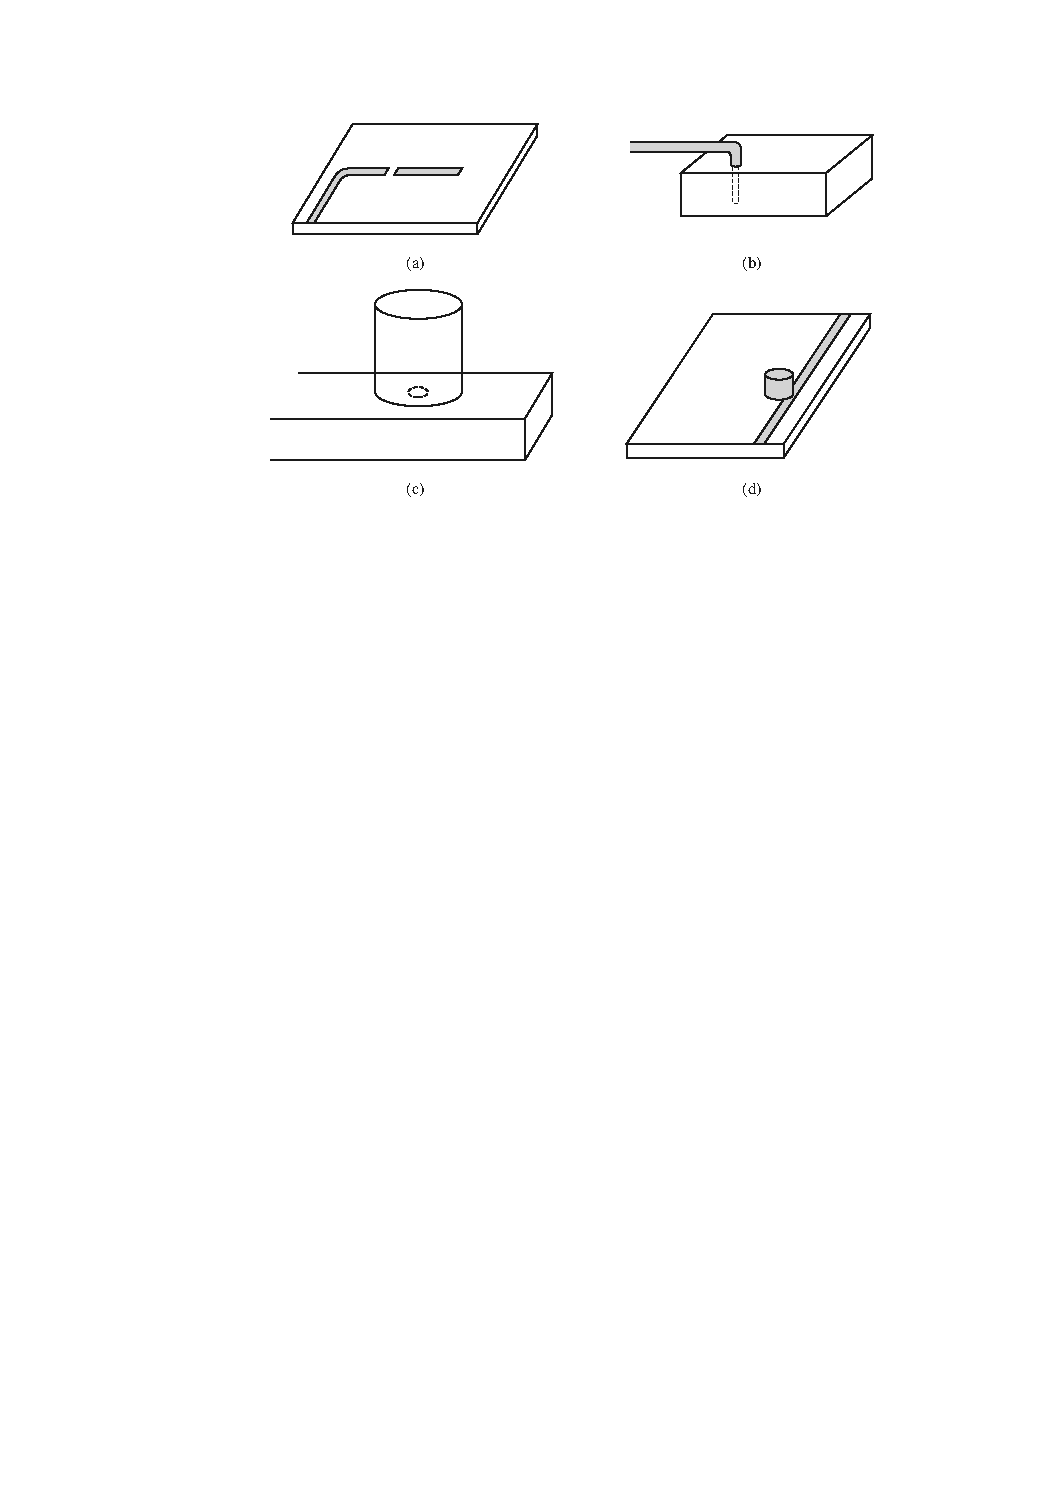
\includegraphics[width=0.7\textwidth]{couplings.pdf}
  \caption{Coupling to microwave resonators, reproduced with permission from \cite{pozar}.}\label{fig:coupling}
\end{figure}

\begin{figure}
\centering
\begin{tikzpicture}
%\draw[step=1cm,gray,very thin] (-3,0) grid (13,7.5);
    \node[anchor=south west,inner sep=0] (image) at (0,0) {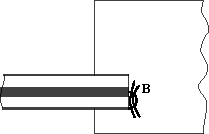
\includegraphics[width=0.4\textwidth]{coupling_loop.pdf}};
    \draw [-latex, thick, red] (1.5,0) node[anchor=east, black] {Coaxial line} to (2.5,0.8);
    \draw [-latex, thick, red] (7,2.5) node[anchor=west, black] {Coupling loop} to (4.25,1);
    \draw [-latex, thick, red] (7,0.4) node[anchor=west, black] {Magnetic field lines} to (4.25,0.75);
    \draw [-latex, thick, red] (2,3) node[anchor=east, black] {Cavity} to (2.9,2.5);
\end{tikzpicture}
\caption{Illustration of a coupling loop.}\label{fig:loop}
\end{figure}

In Fig. \ref{fig:coupling} a few examples for couplings to microwave resonators are shown. Coupling networks usually cater to certain feed lines, modes or desired reactive loads. Fig. \ref{fig:coupling}a shows a gap-coupled microstrip resonator, which couples capacitively from a microstrip to a microstrip resonator. Fig. \ref{fig:coupling}b features an electric probe coupling that couples between a coaxial line and a rectangular waveguide cavity. These two examples were both for (Quasi-)TEM lines, but Fig. \ref{fig:coupling}c exemplifies a rectangular waveguide as feed line and a simple hole in the waveguide as coupling to a cylindrical cavity attached to the waveguide. Finally, Fig. \ref{fig:coupling}d shows a microstrip coupling to a dielectric resonator. Obviously, there is a wide number of different couplings for microwave resonators. For the split-cylinder resonator we have chosen to use magnetic loop coupling (Fig. \ref{fig:loop}). Magnetic loop coupling uses a coaxial line as feed line, which is inserted into the cavity and has the inner conductor connected to either the walls of the cavity or the outer conductor of the feed line. Due to this loop an incident wave creates a loop current in the cavity, which acts more or less like an electrically small magnetic loop antenna.

\begin{figure}
\centering
\begin{circuitikz}
\ctikzset {bipoles/length=0.9cm}
\draw (-2,0) to[short,o-] +(2,0);
% Coupled resonator 1
\draw (0,0) to[short] +(0,-0.25)
			to[L] +(0,-1.5)
			to[short] +(0,-0.25)
			to[open] +(0.5,1.75)
			to[R,l_=$R_1$] +(2,0)
			to[C=$C_1$] +(0,-1.5)
			to[short] +(-2,0)
			to[L,l_=$L_1$] +(0,1.5)
			to[open] +(-0.45,-0.25)
			to [bend left] node[pos=0.5,above] {\tiny $M_{01}$} ++(0.4,0);
% Coupled resonator 2
\draw (0,-2) to[short] +(0,-0.25)
			to[L] +(0,-1.5)
			to[short] +(0,-0.25)
			to[open] +(0.5,1.75)
			to[R,l_=$R_2$] +(2,0)
			to[C=$C_2$] +(0,-1.5)
			to[short] +(-2,0)
			to[L,l_=$L_2$] +(0,1.5)
			to[open] +(-0.45,-0.25)
			to [bend left] node[pos=0.5,above] {\tiny $M_{02}$} ++(0.4,0);
% Dashed line
\draw[dashed] (0,-4) -- +(0,-1);
% Coupled resonator 2
\draw (0,-5) to[short] +(0,-0.25)
			to[L] +(0,-1.5)
			to[short] +(0,-0.25)
			to[open] +(0.5,1.75)
			to[R,l_=$R_n$] +(2,0)
			to[C=$C_n$] +(0,-1.5)
			to[short] +(-2,0)
			to[L,l_=$L_n$] +(0,1.5)
			to[open] +(-0.45,-0.25)
			to [bend left] node[pos=0.5,above] {\tiny $M_{0n}$} ++(0.4,0);
%			
\draw (-2,-7) to[short,o-] +(2,0);

\draw (-1,-3.5) node{$L_0$};



\end{circuitikz}
\caption{Equivalent circuit of a magnetic coupling loop according to \cite{mdp}.}\label{fig:lagrangian}
\end{figure}

Using a Lagrangian method an equivalent circuit (Fig. \ref{fig:lagrangian}) for small loops with an approximately constant loop current can be found \cite{mdp}. The equivalent circuit shows that every mode in the cavity is inductively coupled to the input of the loop by the mutual inductance $M_{0n}$ of a coupled inductor. Equation \eqref{eq:m0n} states that each orthonormal mode $\mathcal{H}_n$ in the cavity with magnetic flux lines running through the loop is coupled out of the cavity. The strength of this coupling depends on the flux running through the loop, the permeability of the field region inside the cavity $\mu$ and the wave number $k_n=\omega_{0n}\sqrt{\epsilon\mu}$.
\begin{equation}\label{eq:m0n}
M_{0n}=\mu k_{0,n}\int\limits_{\mathcal{A}}(\vec{n}\cdot\vec{\mathcal{H}}) dA \qquad \frac{1}{V}\int\limits_{\mathcal{V}}(\vec{\mathcal{H}_n}\cdot\vec{\mathcal{H}_m})dV=\delta_{m,n}
\end{equation}
The other circuit elements of each resonant circuit are defined by the resonant frequency $\omega_{0n}=\frac{1}{\sqrt{L_nC_n}}$ and the quality factor of the mode $Q_n=\frac{\omega_{0n}L_n}{R_n}$, finally the self-inductance of the coupling loop is modelled by the inductor $L_0$.
Regarding the mutual inductance it is interesting to note that the wave number and the permeability are non-zero constants, while the flux through the loop depends on the location and the orientation of coupling loop in the magnetic field. This can be used to amplify or suppress certain modes in a cavity by either locating the coupling loop in an area with a relatively strong field or by turning the loop into the direction of a strong field component. A very useful property, which as we will see in our discussion of the split-cylinder resonator, allows us to separate the transverse magnetic and transverse electric fields of a cavity. 


     % Quality factor measurements
\chapter{Split-Cylinder Resonator}\label{ch:splitc}
\begin{figure}
\centering
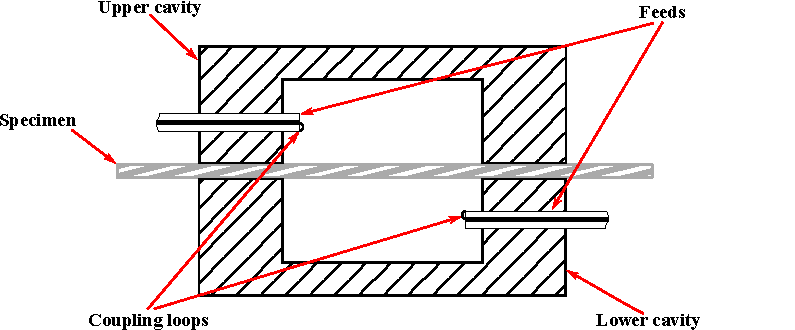
\includegraphics[width=0.8\textwidth]{split_cylinder_resonator.pdf}
\caption{Split-cylinder resonator.}\label{fig:split_cyl}
\end{figure}
In the previous chapters of this thesis we have now covered the fundamentals of permittivity and dielectrics, the dielectric measurement methods at microwave frequencies and the theory of quality factor measurements, but we have not touched the main topic of this thesis, the split-cylinder resonator. Like the resonators mentioned in Chapter \ref{ch:methods}, the split-cylinder resonator is a dielectric measurement method of the standing-wave type. As can be seen in Fig. \ref{fig:split_cyl} the split-cylinder resonator consists of a cylindrical cavity that has been separated into two halves, an upper and a lower cavity. Between the two cavities a relatively thin, flat dielectric specimen is placed, whose dielectric properties are meant to be analysed. Magnetic coupling loops are used to excite the resonator and to measure the resonances of the resonator. The resonant frequencies of one or multiple modes in the cavity are used to calculate the dielectric constant and their quality factors are used to calculate the dielectric loss of the specimen. The specimen only needs to be placed between the two cavities, so it can be measured without any preparation of the specimen. This is unlike many other resonant methods, most of which require machining a specimen in order to fit it into a cavity. This a shared property with a very similar method, the split-post dielectric resonator (see Chapter \ref{ch:methods}). Although the cavity does not cover the entire specimen, the resonator method is still among the most accurate dielectric measurement methods. Achieving a relative uncertainty of the dielectric constant of $u_r(\epsilon)<1\%$ and an uncertainty of the measured loss tangent of $u(\tan\delta )<\num{1e-4}$ at a resolution of less than \num{2e-5} \cite{keysightSC,janezic1999, chen}.

\section{\texorpdfstring{TE\st{0n}}{TE0n} Modes}
\begin{figure}
\centering
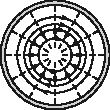
\includegraphics[height=5.35cm]{te01.pdf}
\caption{Radial magnetic field and azimuthal electric field of the $TE_{01}$ mode, adapted with permission from \cite{ramo}.}\label{fig:fc_te}
\end{figure}

A major contributor to the high accuracy of the method are the modes employed by the method. Like many other methods the split-cylinder uses circularly polarised transverse electric (TE) modes, so called TE\st{0n} modes. These modes are a group of field configurations that can exist inside a cylindrical waveguide and that have genuine advantages for dielectric measurements. Firstly, the TE\st{0n} modes of a cylindrical waveguide have the lowest attenuation coefficient of all cylindrical waveguide modes and unlike all other modes their attenuation monotonically decreases with frequency \cite{balanis}. The reason for this lies in the symmetry of the modes, due their azimuthal symmetry (i.e. $\vec{E}=E_{\phi}\vec{e}_\phi$) the magnetic field has only a axial component and radial component, of which only the component tangential to the waveguide walls, the $z$ component $H_z$, contributes to the losses in the waveguide walls. The $H_z$ component is inversely proportional to the frequency, making the attenuation losses along waveguide fall with frequency. Before the advent of modern fibre optical communications with their fundamental HE\st{11} mode and discovery of the near-IR low-loss window of silica, these modes were considered for microwave long-range communications. While cylindrical cavities not only have losses in the waveguide walls but also in the endplates that make up the cavity, they are still the modes with highest quality factors of all modes in cylindrical cavities. As can be seen in Fig. \ref{fig:q_cc} for the first few TE and TM modes, this is also true for most cylindrical waveguide geometries. This makes TE\st{0n} cavities very attractive for the measurement of low-loss dielectrics, since conductor losses are generally lower than in other cavities. The root cause for this is that for resonant dielectric loss measurements the dielectric loss becomes part of the energy balance that defines the quality factor.

\begin{equation}
Q=\frac{\omega_rW}{P_c+P_s} \qquad P_s = (\frac{\omega_rW}{Q}\pm u(\frac{\omega_rW}{Q}))-(P_c\pm u(P_c))
\end{equation}

To measure the dielectric loss, we need to determine the losses in the specimen $P_s$ from a measured resonant frequency and quality factor. We can model the fields in the cavity using appropriate mathematical techniques, which yields an estimate for the field configuration in the cavity. This estimate is then used to compute the energy $W$ in the entire cavity and in the specimen. To compute the losses in the cavity walls $P_c$, we take the  tangential magnetic field $\vec{H}_t$ on the cavity surface from the field configuration and compute the surface loss using the surface resistivity of the cavity walls. To accurately measure the dielectric losses in a cavity, we must accurately account for how much energy is dissipated in the cavity walls and how much is dissipated in specimen. For low-loss dielectrics the specimen loss $P_s$ becomes very small compared to the cavity loss $P_c$, so the uncertainty of the cavity loss estimate can easily dwarf the specimen loss, making the measurement of low-loss dielectrics less and less accurate. If the cavity loss is very low to begin with, the measurement is generally more accurate, reducing the influence of uncertainties arising from the field estimate or from the surface resistance estimate.

\begin{figure}
\centering
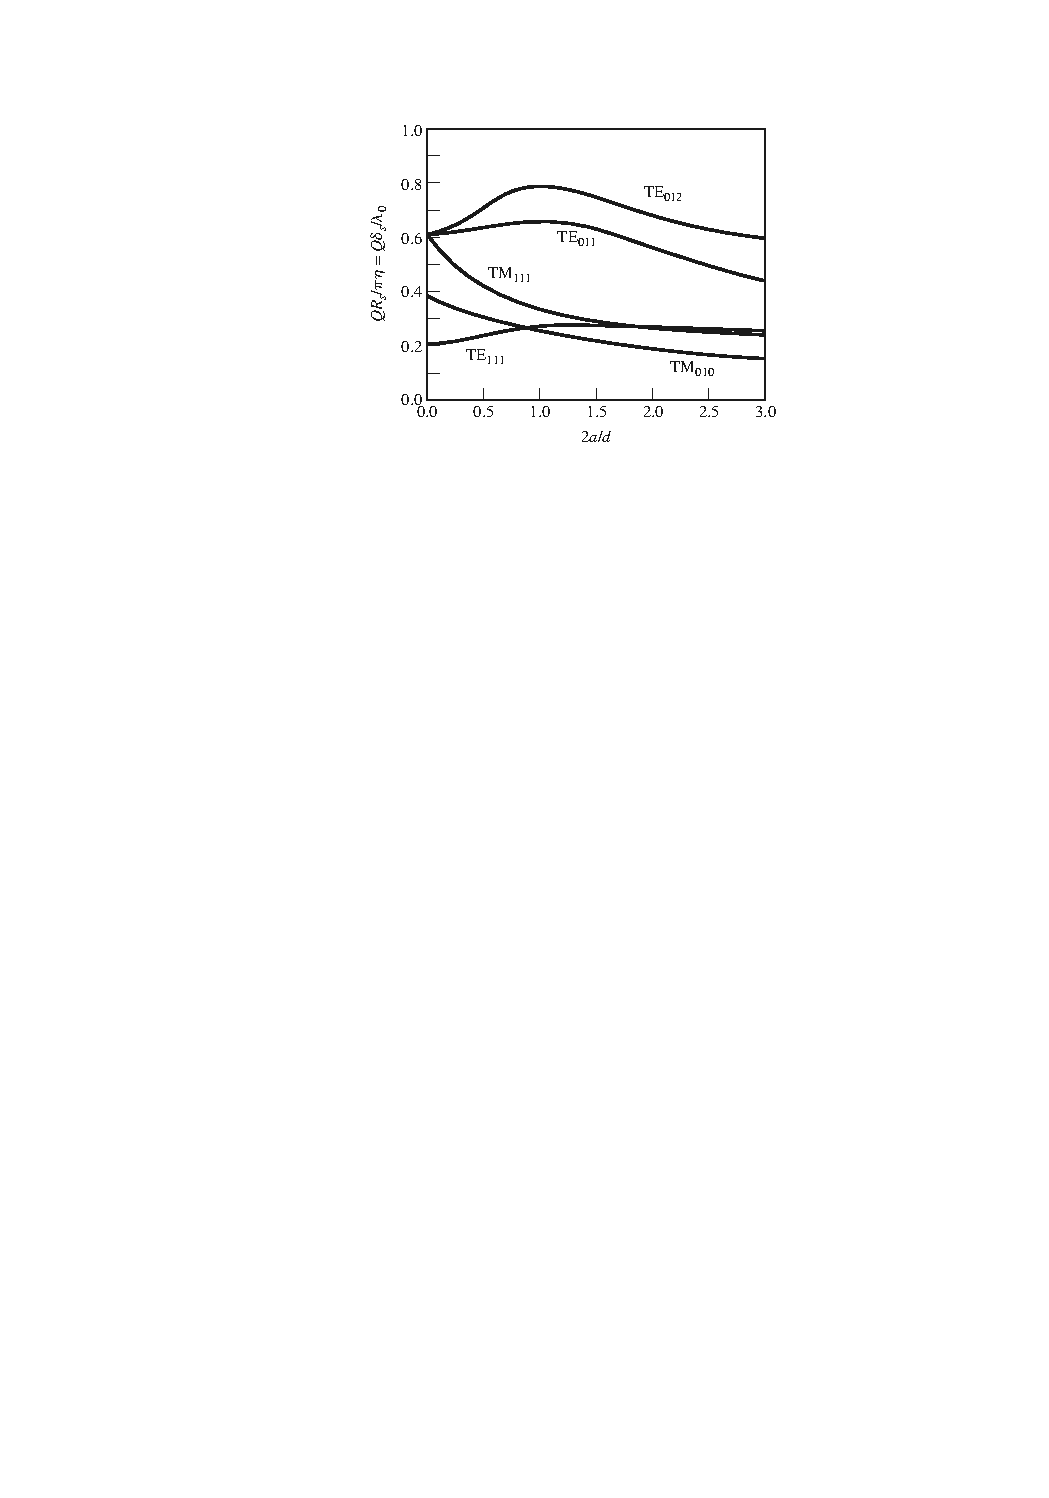
\includegraphics[height=0.27\textheight]{te_modes_q.pdf}
\caption{Normalized quality factors of cylindrical cavity modes for different cavity geometries, reproduced with permission from \cite{pozar}. $2a$ is the diameter of the cavity, and $d$ is the length. The dashed line marks the cavity geometry with the highest normalized quality factor.}\label{fig:q_cc}
\end{figure}

Secondly, the symmetry of the TE\st{0n} modes themselves has a positive influence on measurement accuracy. When measuring dielectrics in microwave cavities a major issue with many techniques are interfaces between dielectric and cavity walls and between dielectric and air. As these interfaces are typically not perfect, but random with numerous air-gaps scattered between the dielectric and the neighbouring material. If the electric field in the field region is perpendicular to these interfaces, the electric field becomes discontinuous and can cause systematic errors in dielectric measurements. Baker-Jarvis et al. \cite{tn1520} stated that measurement fixtures in which the electromagnetic fields are tangential to the air-material interface, such as TE\st{01} cavities and dielectric resonators, generally yield more accurate results than fixtures where the fields are normal to the interface. In the split-cylinder resonator the dielectric is placed in the middle of the resonator with its face directed into the direction of the axis of symmetry. A TE\st{0n} mode propagating from one end of the cavity to the other never encounters an interface where its electric field is normal to that interface, so air-gaps between the dielectric and cavity walls are effectively mitigated. Apart from this positive influence on measurement accuracy, the modes also simplify the measurement of thin materials. These materials typically only interact weakly with the cavity, so the measurement accuracy of thin materials is generally low. Tangential electric modes allow us to stack thin dielectrics hereby increasing the measurement accuracy \cite{NPL}.

Lastly, the field configuration is a good choice for the measurement of anisotropy in dielectrics. As we pointed out in our discussion of dielectric properties of materials at microwave frequencies, at the beginning of Chapter \ref{ch:methods}, many dielectric laminates as well as other materials have a weak anisotropy. These materials typically have different in-plane permittivities and out-of-plane permittivities. The circular polarisation of the mode allows us to directly determine the in-plane permittivity of these dielectrics or an average permittivity if the material is a weakly biaxial dielectric \cite{kent1996}. Unfortunately for many applications in microwave engineering the out-plane permittivity is more important, since the electric field orientation of many planar waveguides is predominantly normal to the surface of the material. To avoid this, two different different cavities can be used to characterise the dielectric, for example a TE\st{01} cavity may be used for the in-plane permittivity and a TM\st{010} cavity may be used for the out-of-plane permittivity \cite{dankov}.
\section{Coupling and Quality Factor Measurements of the Split-Cylinder Resonator}
The advantages of the TE\st{0n} modes has led to the development of various TE\st{01}-mode cavities \cite{NPL}, which are used for dielectric measurements of laminar low-loss dielectrics in the \SIrange{8}{40}{\giga\hertz} range. In this frequency range the microwave cavities can be easily manufactured and are not outperformed by open resonators, which are still relatively large at these frequencies. Many TE\st{01}-mode cavities are closed cavities with a uniform diameter and specimens cut to fit into the inside of the cavity. This simplifies the modelling of the cavities, but makes specimen preparation more complicated. While the split-cylinder resonator and all other TE\st{01}-mode cavities benefit from the TE\st{0n} modes, they also share two major disadvantages. The first disadvantage is that the TE\st{01} mode is not the dominant mode of the cylindrical cavity. Depending on the geometry of the cylindrical cavity, either the TM\st{010} mode or the TE\st{111} mode may be the dominant mode of a cylindrical cavity \cite[Sec. 9.3.2]{balanis}. To measure with TE\st{0n} modes we first need to identify the resonances of the TE\st{0n} modes in a measurement, for example in a transmission coefficient plot. Since the resonant frequencies of the modes depend on the geometry and the dielectric constant of the specimen, we need to estimate the dielectric constant before we can identify the TE\st{0n} modes. Janezic et al. \cite{janezicarz} found out that a fundamental TE\st{111} mode can be used to estimate the dielectric constant in a split-cylinder, but more on that topic later.

The second disadvantage of the TE\st{0n} modes are the degenerate TM\st{1n} modes. These modes are transverse magnetic modes (TM) that have the same dispersion relation as the TE\st{0n} modes, so their resonant frequencies are identical. The magnetic coupling loops of the split-cylinder resonator are used to suppress these degenerate modes. As we have already pointed out in Section \ref{sec:cofc}, the magnetic coupling loop couples only to modes that have magnetic field lines running through the loop. If we turn the face of the loop into the direction of $z$ axis of the resonator, i.e. the z-axis, all TM modes are effectively suppressed.

These modes have the same resonant frequency and a cavity has infinitely many modes with a wide range of different resonant frequencies. This raises the question, how can we measure a single resonance without interference from other modes? Coupling loops tap into all modes with field lines going through the loop. The equivalent circuit of a single loop (ref. Sec. \ref{sec:cofc}) are multiple ideal transformers in series with their secondary winding connected to resonant circuits, which make up the modes of the cavity. A split-cylinder resonator uses two coupling networks. Since the split-cylinder resonator is a measurement resonator, it is only weakly coupled to the rest of the measurement circuit. As have already mentioned, this keeps the modes in the resonator as undisturbed as possible and it allows us to directly measure the unloaded quality factor $Q_0$ of each mode. Unfortunately, reducing the coupling also makes the resonator highly resistive, so we need to use transmission-type quality factor measurements to keep the measurements accurate. Reflection coefficient measurements of highly resistive networks are known to be relatively inaccurate.
\begin{figure}
\centering
\begin{circuitikz}
\ctikzset {bipoles/length=0.9cm}

% Source network
\draw(-3,0) to[short] +(1.5,0)
			to[R=$Y_{01}$] +(0,-4.25);
\draw[dashed] (-1.5,-4.25) -- +(0,-1);
\draw(-1.5,-5.25) to[short] +(0,-2)
			to[short] +(-1.5,0)
			to[short] +(0,2);
\draw[dashed](-3,-5.25) -- +(0,1);
\draw(-3,-4.25)	to[I=$i_s$] +(0,4.25);

% Coupled resonator 1
\draw (0,0) to[short] +(0,-0.25)
			to[L,l_=$n_{11}$] +(0,-1.5)
			to[short] +(0,-0.5)
			to[open] +(0.5,2)
			to[short] +(1,0) node[above] {$Y_1$}
			to[fullgeneric,*-*] +(0,-1.5)
			to[open] +(0,1.5)
			to[short] +(1,0)
			to[open] +(0.5,-2)
			to[short] +(0,+0.5)
			to[L,l_=$n_{21}$] +(0,+1.5)
			to[short] +(0,+0.25)
			to[open] +(-0.5,-0.25)
			to[L,l_=$1$] +(0,-1.5)
			to[short] +(-2,0)
			to[L,l_=$1$] +(0,1.5)
			to[open] +(-0.45,-0.3)
			to [bend left] node[pos=0.5,above] {} ++(0.4,0)
			to[open] +(2.1,0)
			to [bend left] node[pos=0.5,above] {} ++(0.4,0);
			
% Coupled resonator 2
\draw (0,-2.25) to[short] +(0,-0.25)
			to[L,l_=$n_{12}$] +(0,-1.5)
			to[short] +(0,-0.25)
			to[open] +(0.5,1.75)
			to[short] +(1,0) node[above] {$Y_2$}
			to[fullgeneric,*-*] +(0,-1.5)
			to[open] +(0,1.5)
			to[short] +(1,0)
			to[open] +(0.5,-1.75)
			to[short] +(0,+0.25)
			to[L,l_=$n_{22}$] +(0,+1.5)
			to[short] +(0,+0.25)
			to[open] +(-0.5,-0.25)
			to[L,l_=$1$] +(0,-1.5)
			to[short] +(-2,0)
			to[L,l_=$1$] +(0,1.5)
			to[open] +(-0.45,-0.3)
			to [bend left] node[pos=0.5,above] {} ++(0.4,0)
			to[open] +(2.1,0)
			to [bend left] node[pos=0.5,above] {} ++(0.4,0);
% Dashed line
\draw[dashed] (0,-4.25) -- +(0,-1);
\draw[dashed] (3,-4.25) -- +(0,-1);
% Coupled resonator 3
\draw (0,-5.25) to[short] +(0,-0.25)
			to[L,l_=$n_{1N}$] +(0,-1.5)
			to[short] +(0,-0.25)
			to[open] +(0.5,1.75)
			to[short] +(1,0) node[above] {$Y_N$}
			to[fullgeneric,*-*] +(0,-1.5)
			to[open] +(0,1.5)
			to[short] +(1,0)
			to[open] +(0.5,-1.75)
			to[short] +(0,+0.25)
			to[L,l_=$n_{2N}$] +(0,+1.5)
			to[short] +(0,+0.25)
			to[open] +(-0.5,-0.25)
			to[L,l_=$1$] +(0,-1.5)
			to[short] +(-2,0)
			to[L,l_=$1$] +(0,1.5)
			to[open] +(-0.45,-0.3)
			to [bend left] node[pos=0.5,above] {} ++(0.4,0)
			to[open] +(2.1,0)
			to [bend left] node[pos=0.5,above] {} ++(0.4,0);

% Connection networks
\draw (-1.5,0) to[short,*-] +(1.5,0);
\draw (-1.5,-7.25) to[short,*-] +(1.5,0);
% Load network
\draw (3,0) to[short] +(1.5,0)
			to[R=$Y_{02}$] +(0,-4.25)
			to[open] +(0,-1)
			to[short] +(0,-2)
			to[short] +(-1.5,0);
\draw[dashed] (4.5,-4.25) -- +(0,-1); 

% Resonant circuit
\draw (6,-2) to[fullgeneric=$Y_n$,o-o] +(0,-2);
\draw[double, latex-latex] (7,-3) to +(1.5,0);

\draw (10,-4.25) to[short,o-] +(0,+0.5)
			to[short] +(1,0)
			to[C,l_=$C_n$] +(0,1.5)
			to[short,-*] +(-1,0)
			to[short] +(-1,0)
			to[R=$R_n$] +(0,-1.5)
			to[short,-*] +(1,0)
			to[L,l_=$L_n$] +(0,1.5)
			to[short,-o] +(0,+0.5);


\end{circuitikz}
\caption{Equivalent circuit of the Split-Cylinder resonator.}\label{fig:splitc_model}
\end{figure}
To model the filtering of unwanted TM modes and the interference from neighbouring modes, we can use the equivalent circuit of the split-cylinder resonator of Fig. \ref{fig:splitc_model}. The circuit uses ideal transformers in series at the input and the output of the resonator, which all have RLC resonant circuits on their secondary winding. Unlike the equivalent circuit of the coupling loop that we discussed in Sec. \ref{sec:cofc}, this resonator is under-coupled, so the self-inductances of both loops become negligible. The resonant circuits and the ideal transformers remain. The coupling coefficient of each ideal transformer depends on the magnetic field strength of the mode on its secondary winding. TM modes and also TE modes with a field minimum along the z-axis have very small coupling coefficients. 

The result of a transmission-type quality factor measurement of a split-cylinder resonator is a transmission coefficient plot that is a superposition of all modes that couple to the coupling loop. The resonance condition of such a resonator is unlike that of a simple RLC resonant circuit. An accurate measurement of the resonant frequency and the quality factor of a mode is only possible if the measurement mode is the only mode oscillating in a certain frequency range. We can calculate the transmission coefficient of the equivalent circuit of Fig. \ref{fig:splitc_model} to get an expression for the superposition of all modes
\begin{equation}\label{eq:s_modes}
S_{21}(\omega)=\frac{2\sqrt{Y_{01}Y_{02}}\left(\sum\limits_{n=1}^{N}\frac{n_{1n}n_{2n}}{Y_n}\right)}{1+\sum\limits_{n=1}^{N}\left(\frac{n_{1n}^2Y_{01}}{Y_n}+\frac{n_{2n}^2Y_{02}}{Y_n}\right)+\sum\limits_{n=1}^{N}\sum\limits_{\substack{k=1 \\ n\neq k}}^{N}\frac{Y_{01}Y_{02}\left(n_{1n}n_{2k}-n_{2n}n_{1k} \right)^2}{Y_nY_k}} \text{,}
\end{equation}
where
\begin{equation}
Y_n(\omega)=G_{0,n}(1+jQ_{0,n}\delta_n) \quad \text{and} \quad \delta_n = \frac{\omega}{\omega_{r,n}}-\frac{\omega_{r,n}}{\omega}\text{.}
\end{equation}
Using Eq. \eqref{eq:s_modes} we can show that multiple modes may be resolved through careful fitting or that individual modes may be measured if they are undisturbed, i.e. do not overlap with neighbouring modes. In our measurements with the split-cylinder resonator we decided to use only undisturbed modes to simplify the matter. An undisturbed mode requires all neighbouring modes to have either minuscule coupling like in the case of the degenerate TM modes ($n_{1n}\rightarrow 0$ or $n_{2n}\rightarrow 0$) or a relatively small bandwidth of the resonance curve so that we can assume $Y_n\rightarrow\infty$ for all neighbouring modes in the vicinity of the mode. In these two cases Equation \eqref{eq:s_modes} simplifies to
\begin{equation}
S_{21}(\omega)=\frac{2\sqrt{n_{11}^2Y_{01}n_{21}^2Y_{02}}}{n_{11}^2Y_{01}+n_{21}^2Y_{02}+G_{0,1}(1+jQ_{0,1}\delta_1)}\text{,}
\end{equation}
which is the same result as in the case of the transmission-type measurement of a single RLC resonant circuit.(cf. Eq. \eqref{eq:tr_S}) This proves that a single mode can be accurately measured as long as the mode is undisturbed.

For these derivations we assumed that the resonator was very under-coupled. This implied that the inductance of the coupling loop became negligible, so the inductive loading of the resonator disappeared. In our measurements we also observed that the resonant frequency converged to a constant value when we reduced the coupling. The resistive loading on the other hand did not disappear, since we still need to couple power through the resonator for our measurements! Resistive loading has the downside that it changes the quality factor, so our assumption that the loaded quality factor is equal to the unloaded quality factor is not entirely valid. There is a trade-off between having enough coupling to accurately measure a resonance curve, and keeping the coupling weak enough to ensure $Q_L\approx Q_0$. Janezic \cite{janezic} suggested that a peak transmission coefficient of less than \SI{-50}{\decibel} was a good compromise between the two criteria. In our measurements we found that a coupling level of \SIrange{-70}{-50}{\decibel} was often a good choice. At these coupling levels we can show for symmetric coupling
\begin{equation}
n_{11}^2Y_{01}=n_{21}^2Y_{02}=Y'
\end{equation}
\begin{equation}
S_{21}(\omega)=\frac{2\sqrt{n_{11}^2Y_{01}n_{21}^2Y_{02}}}{n_{11}^2Y_{01}+n_{21}^2Y_{02}+G_{0,1}(1+jQ_{0,1}\delta_1)}=\frac{\frac{1}{1+\frac{G_{0,1}}{2Y'}}}{1+j\frac{Q_{0,1}\delta_1}{1+\frac{2Y'}{G_{0,1}}}}\text{.}
\end{equation}
If we take the peak coupling levels of our measurements, we yield the coupling coefficient
\begin{equation}
S_{21}(\omega_r)=\frac{1}{1+\frac{G_{0,1}}{2Y'}} \Rightarrow \frac{2Y'}{G_{0,1}}=2\kappa=\frac{1}{\frac{1}{S_{21}(\omega_r)}-1}=\num{3.16e-4}\ ...\ \num{3.17e-3}
\end{equation} 
and the unloaded quality factor 
\begin{equation}
Q_0=(\num{1.00032}\ ...\ \num{1.00317})Q_L
\end{equation} of the resonator at these levels. Thus, we have shown that the coupling coefficient has a small influence on our quality factor measurements, but as we will see when discuss our measurement results the influence of the coupling is generally negligible. 
\section{Modelling the Split-Cylinder Resonator}\label{sec:modelling}
In this section we now address the electro-magnetic modelling of the split-cylinder resonator. Ermert \cite{ermert}, Guillon \cite{guillon}, Koba\-yashi \cite{kobayashi} and Kent \cite{kent1996} were among the first to analyse the split-cylinder resonator. Kent developed a split-cylinder resonator that he called resonant dielectrometer, which built on the available research in the area of TE\st{0n} cavities. He used coupling loops to suppress the degenerate TM modes. He proposed to measure the permittivity by at first modelling the cavity as a closed cavity with uniform diameter and then correcting the error of the model with a gap correction. The permittivity of a sample in a closed cavity was computed using a simple Eigenvalue problem and the gap correction was derived from a perturbation calculation. \cite{kent1996gap} Kobayashi used a very similar model, although he computed a gap-correction using a Rayleigh-Ritz method and suggested using a PTFE ring in the cavity as a mode filter for the degenerate TM\st{11} modes.

Janezic \cite{janezic1999} later derived a full-wave model of the split-cylinder resonator. Like the other authors he recognised that the boundary value problem extends into the outside of the cavity and proposed an infinitely large sample radius as an approximation for this boundary value problem. The sample was supposed to backed by a infinitely large flange confining all the fields to the sample and the cavity. For the modes he assumed that TE\st{0n} modes excite only TE\st{0n} modes and that the modes in the cavity can be represented by a series expansion of TE\st{0n} modes. He used a Hankel transform to solve the field problem and showed that the approximation is correct for relatively large, thin specimens. Although convergence was achieved with a small number of modes, the wall losses were omitted in the model to limit computational complexity. 

For his PhD thesis Janezic \cite{janezic} studied the split-cylinder resonator in detail and compared three theoretical models for the resonator. The three models were a mode-matching model, a least-squares boundary residual model (LSBR) and a Hankel-transform model. For the mode-matching and the LSBR model he modelled the the cavity as a closed cavity with a perfectly conducting boundary at $\rho=b$ in the sample region and a perfectly conducting flange ranging from the cavity diameter to the the perfectly conducting boundary at $\rho=b$. He recognised that this assumption simplified the calculations greatly and led only to a small systematic error in the measurements. His Hankel transform model used the same boundary conditions as his original model \cite{janezic1999}, so he also assumed an infinitely large sample radius and an infinitely large flange. Unlike in his original model the loss calculations of all models also included the losses of the cavity. He compared all three models in terms of the satisfaction of boundary conditions, the accuracy of the measured relative permittivity, the accuracy of the measured loss tangent and the computational speed of the model. The mode-matching model was selected as the best model, because it was the fastest model and also computed the complex permittivity accurately. As far as the other methods were concerned, the least-squares boundary residual model was found to be fast, but the accuracy of the computed permittivities was generally poor due to problems with the weighing functions of the model. The Hankel transform model showed some potential, but the computation of the Hankel transforms was very slow and the loss calculations neglected the flange loss due to problems with the numerical integration of a Hankel transform. Janezic also made a few measurements with the mode-matching model in which the model generally performed very well. He also added a uncertainty calculation for the mode-matching model.

The convenience and accuracy of the split-cylinder method has also gained the interest of the circuit board and dielectric substrate industry. This has led to the standardisation of Kobayashi's model and of Janezic's mode-matching model. Kobayashi's model was first standardised in 2002 as Japanese standard JIS R 1641 \cite{kobayashistandard} and subsequently in 2011 as IEC standard IEC 62562 \cite{iecSC}. The mode-matching model was standardised in 2007 as IPC test method TM-650 2.5.5.13 \cite{ipcSC}. Keysight \cite{keysightSC} also implemented a split-cylinder resonator based on Janezic's mode-matching model.

Recently two new models for the split-cylinder resonator were published, which both aimed at improving the mode identification of the split-cylinder resonator. Although the mode-matching model and the other models are very accurate and well understood, they only calculate the TE\st{0np} modes of the resonator. As we have already mentioned before, the TE\st{011} mode is not the dominant mode of the resonator, so one approach is to estimate the dielectric constant from the dominant TE\st{111} mode and then calculate the resonant frequency of the higher modes from this estimate. The calculated resonant frequencies are in turn used to find the resonant frequencies in our measurements and compute the actual dielectric constant \cite{janezicarz}. This approach is acceptable as long as the dielectric constant varies only slowly over frequency, which is the case for all low-loss dielectric (cf. Chapter \ref{ch:methods}), and as long as only one resonance of transmission coefficient lies close to the calculated resonant frequency. If more than one resonance curve lies close to the calculated resonant frequency, this method fails. A model for all TE and TM modes would allow us to identify all modes, even if two modes lie very close to each other. For this purpose Zinal \cite{zinal} proposed an extended mode-matching model, which included all TE and TM modes. Since he neglected the fringing fields in his calculations, the model was less accurate than others models. Villaroya \cite{villaroya1,villaroya2} also published a model for all TE and TM modes. His model used a full-wave circuit method that also used the same boundary conditions as Janezic's mode-matching model. In his article he only used TE\st{0np} modes for his complex permittivity measurements, since he recognised that the uncertainty of $\tan\delta$ measurements with other TE modes was generally too high. He published his model only a few months before the publication of this thesis, so it still remains to be seen whether his model can both accurately measure the TE\st{0np} modes and identify all modes of split-cylinder resonator.
     % Split Cylinder Resonator
\chapter{An Asymmetric Mode-Matching Model}\label{ch:m12}
As we have discussed the split-cylinder resonator is a very accurate and well-researched dielectric measurement method. In our research on the split-cylinder resonator we implemented Janezic's mode-matching model, since it is a widely accepted and well-documented model developed at the renowned American metrology institute NIST. We also manufactured a split-cylinder prototype at our institute's work shop, which confronted us with the limited manufacturing precision of our equipment. Since the mode-matching model assumed a symmetric resonator with two identical cavities at the top and at the bottom, the accuracy of our split-cylinder was very much in doubt. We recognised that a major drawback of the method was the relatively costly production of the cavity. Lower manufacturing cost would allow us to tailor a cylinder to each specimen. This would also circumvent the issues surrounding the large detuning of split-cylinder resonators with thick samples and higher permittivities. Each cavity could be built to have its first TE\st{0np} measurement mode around a certain frequency. This encouraged us to expand and modify the mode-matching model to asymmetric split-cylinders, since the variations in diameter and length of the upper and lower cavities were identified as a potential root of systematic error. For these modifications we had to expand the mode-matching model and change the calibration procedure, both of which we will now derive in this chapter. 
\section{Fields of the Measurement Model}
\begin{figure}
\centering
\begin{tikzpicture}
   %\draw[step=1cm,gray,very thin] (-3,0) grid (13,7.5);
    \node[anchor=south west,inner sep=0] (image) at (0,0) {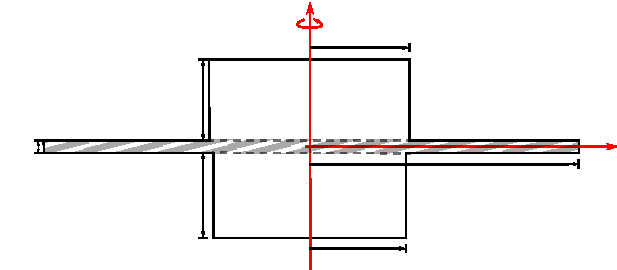
\includegraphics[width=10cm]{split_cylinder_resonator_model.pdf}};
    \draw (5,4.6) node[red] {\textit{z}};
    \draw (10.25,2) node[red] {\textit{$\rho$}};
    \draw (3,2.75) node {$L_u$};
    \draw (3,1.25) node {$L_l$};
    \draw (0.25,2) node {$d$};
    \draw (5.75,3.8) node {$a_u$};
    \draw (5.75,0.1) node {$a_l$};
    \draw (8,1.5) node {$b$};
    
    \draw (3.75,2.75) node[anchor=west] {\scalebox{0.75}{$\mu_0,\epsilon_{lab}$}};
    \draw (3.75,1.25) node[anchor=west]  {\scalebox{0.75}{$\mu_0,\epsilon_{lab}$}};
    \draw (3.75,2) node[anchor=west]  {\scalebox{0.75}{$\mu_0,\epsilon_{s}$}};
\end{tikzpicture}
\caption{Geometry of an asymmetric split-cylinder resonator.}\label{fig:a_SC}
\end{figure}

Janezic \cite{janezic} derived an accurate model for the split-cylinder resonator, which used mode-matching to compute the field configuration in the cavity. Mode-matching is a popular method of computer-aided electro-magnetics \cite{sorrentino, arndt}, which uses the eigenmode expansion of the modes in a region to enforce the boundary conditions at the interface to another region. For the expansion we first need the eigenmodes of each region, so the method requires solutions of the boundary value problem in each region to work. The starting point for our boundary value problem is the electro-magnetic model and geometry of an asymmetric split-cylinder resonator shown in Fig. \ref{fig:a_SC}. The split-cylinder resonator is dielectric measurement method for thin, low-loss dielectric sheets. Its model consists of three open cylindrical cavities that are aligned along a common z-axis. The cavities are an upper-cavity with diameter $2a_u$ and length $L_u$, a sample region with diameter $2b$ and length $d$ and a lower cavity with diameter $2a_l$ and length $L_l$. There two step-discontinuities, one at the interface between upper cavity and sample region and another one between the lower cavity and the sample region. At these interfaces the diameter of the cavity changes abruptly creating a conductive flange at the interface. In terms of materials the cavities are filled with air and the sample region with a linear, homogeneous, isotropic and lossy dielectric, so $\mu=\mu_0$ and $\epsilon_{lab}=1.00055\,\epsilon_0$ may be assumed for the cavities and $\mu=\mu_0$ and $\underline{\epsilon_s}=(\epsilon_r-j\epsilon_r\tan\delta)\epsilon_0$ for the sample region \cite{phillips}. The entire cavity is enclosed by a good conductor with conductance $\sigma$.

To compute the mode-matching model our first step is to solve the boundary value problem of the cylindrical cavities. The wave equation of time-harmonic electric fields in a source- free medium is
\begin{equation}
\nabla^2\vec{E}=\gamma^2\vec{E} \quad\text{with}\quad \gamma=j\omega\mu_0(\sigma+j\omega\epsilon)=j\omega\mu_0(\omega\epsilon''+j\omega\epsilon ')=\omega^2\mu_0\epsilon '(j\tan\delta - 1)\text{,}
\end{equation}
where $\gamma$ is the separation constant of the partial differential equation. We assume that the influence the dielectrics loss of the low-loss dielectrics on the field configurations is negligible, i.e. $\tan\delta=0$,
\begin{equation}\label{eq:wave}
\nabla^2\vec{E}=-k^2\vec{E} \quad \text{and} \quad k=\omega^2\mu_0\epsilon '\text{.}
\end{equation}
From Equation \eqref{eq:wave} the TE and TM eigenmodes of a cylindrical coordinate system can be obtained, of which we are only interested in the TE modes. Using an electric vector potential $\vec{E}=\nabla\times\vec{F}$ and $\vec{F}=F_z\vec{e_z}$ solutions for the TE modes of the wave equation in cylindrical coordinates can be found
\begin{gather}
F_z=\left(A_1J_m(h_n\rho)+B_1Y_m(h_n\rho)\right)\left(C_2\cos(m\phi)+D_2\sin(m\phi)\right)\left(A_3\cos(p_nz)+B_3sin(p_nz)\right)\text{,}\\
k^2=h_n^2+p_n^2\text{,}
\end{gather}
where $J_m$ and $Y_m$ are the mth order Bessel function of the first and second kind, and $A_1$, $B_1$, $C_2$, $D_2$, $A_3$ and $B_3$ are constants. With the curl of $\vec{F}$ we also yield the $\phi$ component of the electric field $E_\phi$
\begin{equation}\begin{split}
E_\phi(\rho,\phi,z)=\frac{1}{\epsilon}\frac{\partial F_z}{\partial\rho}=\frac{1}{\epsilon}\left(A_1h_nJ'_m(h_n\rho)+B_1h_nY'_m(h_n\rho)\right)\left(C_2\cos(m\phi)+D_2\sin(m\phi)\right) \\ \times\left(A_3\cos(p_nz)+B_3sin(p_nz)\right)\text{,}\end{split}
\end{equation}
where $'$ indicate the derivatives of the functions \cite{balanis}. We determine the constants using simplified boundary conditions. We assume that the cavity walls are perfect electric conductors with $\vec{n}\times\vec{E}=\vec{0}$ on the cavity walls. We neglect the influence of lossy walls on the field configuration and we will re-introduce the cavity losses in the loss calculations. A widely accepted simplification that introduces only a minor error in the resonant frequency \cite{collin}. Furthermore, we are only interested in the TE\st{0n} modes of the cavity and since all our cavities are aligned along a common z-axis the TE\st{0n} modes at each interface are orthogonal to all other modes but the TE\st{0n} modes in the other cavity. This special property allows us to expand the fields in the entire cavity in terms of TE\st{0n} modes only, i.e. $\vec{E}=\sum_{n=1}^{\infty}E_{\phi,TE0n}\vec{e_\phi}$. 
The fields in the entire cavity therefore must satisfy:
\begin{enumerate}
\item Azimuthal symmetry of all modes $\Rightarrow m=0 \ \text{and}\ J'_{m=0}(h_n\rho)=-J_1(h_n\rho)$, due to one of the recurrence relations of the Bessel functions
\item Finite fields in the entire cavity $\lim_{\rho\rightarrow 0}Y_m'(h_n\rho)=\lim_{\rho\rightarrow 0}\{Y_{m-1}(h_n\rho)-Y_{m+1}(h_n\rho)\}\rightarrow \infty \Rightarrow B_1=0$
\end{enumerate}
\begin{equation}\label{eq:sol_simple}
E_{\phi}(\rho,z)=\sum\limits_{n=1}^{\infty} \frac{A_nh_n}{\epsilon}J_1(h_n\rho)[A_3\cos(p_nz)+B_3\sin(p_nz)]
\end{equation}
With the simplified solution of Equation \eqref{eq:sol_simple} we can solve the boundary value problem in each cavity with respect to the cavity walls.

Solving the \textbf{upper-cavity} boundary value problem
\begin{gather}
\vec{E}\left(\rho=a_u,\frac{d}{2}\leq z\leq\frac{d}{2}+L_u\right)=\vec{0}\\
\vec{E}\left(0\leq\rho\leq a_u,z=\frac{d}{2}+L_u\right)=\vec{0}\\
\end{gather}
we find a solution for the electric field in the upper cavity
\begin{align}\label{eq:e_u}
E_{\phi,u}(\rho,z)&=\sum\limits_{n=1}^{\infty} A_nU_nJ_1(h_{n,u}\rho)\sin(p_{n,u}\left(L_u+\frac{d}{2}-z\right)), &\scriptstyle (0\leq\rho\leq a_u)\wedge\left(\frac{d}{2}\leq z\leq\frac{d}{2}+L_u\right)
\end{align}
where
\begin{equation}
h_{n,u}=\{\forall h_n\in\mathbb{R}^+:J_1(h_na_u)=0\}\text{.}
\end{equation}
Using this solution we calculate the magnetic fields in the upper cavity,
\begin{align}\label{eq:h_u}
H_{\rho,u}(\rho,z)&=\frac{1}{j\omega\mu_0}\frac{\partial E_{\phi,u}}{\partial z}\\&=\sum\limits_{n=1}^{\infty}\frac{-p_{n,u}}{j\omega\mu_0}A_nU_nJ_1(h_{n,u}\rho)\cos(p_{n,u}\left(L_u+\frac{d}{2}-z\right)),&\scriptstyle\left(0\leq\rho\leq a_u\right)\wedge\left(\frac{d}{2}\leq z\leq\frac{d}{2}+L_u\right)\\
H_{z,u}(\rho,z)&=\frac{-1}{j\omega\mu_0}\left(\frac{1}{\rho}E_{\phi,u}+\frac{\partial E_{\phi,u}}{\partial\rho}\right)\\&=\frac{-1}{j\omega\mu_0}\sum\limits_{n=1}^\infty A_nU_nh_{n,u}J_0(h_{n,u}\rho)\sin(p_{n,u}\left(L_u+\frac{d}{2}-z\right)),&\scriptstyle(0\leq\rho\leq a_u)\wedge\left(\frac{d}{2}\leq z\leq\frac{d}{2}+L_u\right)
\end{align}
In a similar fashion the boundary value of the \textbf{sample region}
\begin{gather}
\vec{E}\left(\rho=b,-\frac{d}{2}\leq z\leq\frac{d}{2}\right)=\vec{0}
\end{gather}
yields the electric field in the sample region
\begin{align}\label{eq:e_s}
E_{\phi,s}(\rho,z)&=\sum\limits_{m=1}^{\infty} J_1(h_{m,s}\rho)\left(B_mV_m\cos(p_{m,s}z)+C_mW_m\sin(p_{m,s}z)\right),&\scriptstyle(0\leq\rho\leq b)\wedge\left(-\frac{d}{2}\leq z\leq\frac{d}{2}\right)
\end{align}
where
\begin{equation}
h_{m,s}=\{\forall h_m\in\mathbb{R}^+:J_1(h_mb)=0\}\text{.}
\end{equation}
Again, the solution allows us to calculate the magnetic field, so in the sample region we obtain
\begin{align}\label{eq:h_s}
H_{\rho,s}(\rho,z)&=\frac{1}{j\omega\mu_0}\frac{\partial E_{\phi,s}}{\partial z}\\&=\sum\limits_{m=1}^{\infty}\frac{p_{m,s}}{j\omega\mu_0}J_1(h_{m,s}\rho)\left(-B_mV_m\sin(p_{m,s}z)+C_mW_m\cos(p_{m,s}z)\right),&\scriptstyle(0\leq\rho\leq b)\wedge\left(-\frac{d}{2}\leq z\leq\frac{d}{2}\right)\\
H_{z,s}(\rho,z)&=-\frac{1}{j\omega\mu_0}\left(\frac{1}{\rho}E_{\phi,s}+\frac{\partial E_{\phi,s}}{\partial\rho}\right)\\&=\sum\limits_{m=1}^\infty \frac{-h_{m,s}}{j\omega\mu_0}J_0(h_{m,s}\rho)\left(B_mV_m\cos(p_{m,s}z)+C_mW_m\sin(p_{m,s}z))\right), &\scriptstyle((0\leq\rho\leq b)\wedge\left(-\frac{d}{2}\leq z\leq\frac{d}{2}\right)
\end{align}
Lastly, the boundary values of the \textbf{lower cavity}
\begin{gather}
\vec{E}\left(\rho=a_l,-\frac{d}{2}\leq z\leq-\frac{d}{2}-L_l\right)=\vec{0}\\
\vec{E}\left(0\leq\rho\leq a_l,z=-\frac{d}{2}-L_u\right)=\vec{0}
\end{gather}
yield a very similar result for the electric field in the lower cavity as in the case of the upper cavity
\begin{align}\label{eq:e_l}
E_{\phi,l}(\rho,z)&=\sum\limits_{p=1}^{\infty} D_pL_pJ_1(h_{p,l}\rho)\sin(p_{p,l}\left(z+L_l+\frac{d}{2}\right)), & \scriptstyle(0\leq\rho\leq a_l)\wedge\left(-\frac{d}{2}-L_l\leq z\leq-\frac{d}{2}\right)
\end{align}
where
\begin{equation}
h_{p,l}=\{\forall h_p\in\mathbb{R}^+:J_1(h_pa_l)=0\}\text{.}
\end{equation}
Similarly, we yield the following for the magnetic field in the lower cavity
\begin{align}\label{eq:h_l}
H_{\rho,l}(\rho,z)&=\frac{1}{j\omega\mu_0}\frac{\partial E_{\phi,l}}{\partial z}\\&=\sum\limits_{p=1}^{\infty}\frac{p_{p,l}}{j\omega\mu_0}D_pL_pJ_1(h_{p,l}\rho)\cos(p_{p,l}\left(z+\frac{d}{2}+L_l\right)), &\scriptstyle(0\leq\rho\leq a_l)\wedge\left(-\frac{d}{2}-L_l\leq z\leq-\frac{d}{2}\right)\\
H_{z,l}(\rho,z)&=\frac{-1}{j\omega\mu_0}\left(\frac{1}{\rho}E_{\phi,l}+\frac{\partial E_{\phi,l}}{\partial\rho}\right)\\&=\frac{-1}{j\omega\mu_0}\sum\limits_{p=1}^\infty D_pL_ph_{p,l}J_0(h_{p,l}\rho)\sin(p_{p,l}\left(z+\frac{d}{2}+L_l\right)), &\scriptstyle(0\leq\rho\leq a_l)\wedge\left(-\frac{d}{2}-L_l\leq z\leq-\frac{d}{2}\right)
\end{align}
For the derivations of the electric fields we merged all constants to common coefficients $A_n$, $B_m$, $C_m$ and $D_p$, and combined them with conditioning coefficient $U_n$, $V_m$, $W_m$ and $D_p$, which will be useful later on.
\subsection{Mode-Matching at the Cavity Interfaces}
With the eigenmode expansion of TE\st{0n} modes in each region at hand, we can now compute the field in the entire cavity. To achieve this we must choose the eigenmode expansion coefficients $A_n$, $B_m$, $C_m$ and $D_p$ as such that the boundary conditions at the interfaces are enforced. The key to this expansion is the orthogonality of the transverse electric fields in a lossless waveguide \cite[Ch. 5.1]{collinFT}. The orthogonality relation of the transverse electro-magnetic fields is the scalar product of the transverse electric field of mode $n$ and the transverse magnetic field of mode $m$, in case of the upper cavity this is the following relation:
\begin{equation}\label{eq:o_u}
\int\limits_0^{2\pi}\int\limits_0^{a_u} E_{\phi,u}^{(n)}H_{\rho,u}^{(m)} \rho d\rho d\phi=K_1\delta_{mm}
\end{equation}
For the sample region the orthogonality relation is
\begin{equation}\label{eq:o_s}
\int\limits_0^{2\pi}\int\limits_0^{b} E_{\phi,s}^{(n)}H_{\rho,s}^{(m)} \rho d\rho d\phi=K_2\delta_{mm}
\end{equation}
and for the lower cavity it is
\begin{equation}\label{eq:o_l}
\int\limits_0^{2\pi}\int\limits_0^{a_l} E_{\phi,l}^{(n)}H_{\rho,l}^{(m)} \rho d\rho d\phi=K_3\delta_{mm}\text{,}
\end{equation}
where $K_1$, $K_2$ and $K_3$ are constants.

The first boundary conditions we need to enforce are at the interface between the upper cavity and the sample region. We demand that the tangential electric field must be continuous across the opening and zero along the perfectly conductive flange, so
\begin{align}\label{eq:bc_1}
E_{\phi,s}\left(\rho,z=\frac{d}{2}\right)= \begin{cases}
    E_{\phi,u}(\rho,z=\frac{d}{2}) , & 0\leq\rho\leq a_u\\
    0, & a_u\leq\rho\leq b
  \end{cases}
\end{align}
must apply. If we insert Equation \eqref{eq:e_l} and \eqref{eq:e_s} into \eqref{eq:bc_1}, we yield
\begin{gather}\label{eq:bc_12}
\sum_{m'=1}^\infty J_1(h_{m',s}\rho)\left\{B_{m'}V_{m'}\cos\left(p_{m',s}\frac{d}{2}\right)+C_{m'}W_{m'}\sin\left(p_{m',s}\frac{d}{2}\right)\right\}=\nonumber\\ \begin{cases}
	\sum_{n=1}^\infty A_nU_nJ_1(h_{n,u}sin(p_{n,u}L_u),&0\leq\rho\leq a_u\\0,& a_u\leq\rho\leq b
\end{cases}
\end{gather}
Next we calculate the scalar product of each side of Equation \eqref{eq:bc_12} and the tangential magnetic field of a mode m from the sample region, for which we multiply both sides with $H_{\rho,s}^{(m)}$  and integrate the expression over the entire surface of the boundary. Due to the orthogonality of the electro-magnetic modes we yield
\begin{gather}
\sum_{n=1}^\infty A_nU_n\frac{a_uh_{n,u}}{h_{m,s}^2-h_{n,u}^2}J_0(h_{n,u}a_u)J_1(h_{m,s}a_u)\sin(p_{n,u}L_u)\nonumber\\=\frac{b^2}{2}J_0(h_{m,s}b)^2\left\{ B_mV_m\cos(p_{m,s}\frac{d}{2})+C_mW_m\sin(p_{m,s}\frac{d}{2})\right\}\text{.}\label{eq:mm_1}
\end{gather}
We also expect the tangential magnetic field to be continuous across the interface of the upper cavity with the sample region, this implies
\begin{equation}\label{eq:bc_2}
H_{\rho,s}\left(\rho,z=\frac{d}{2}\right)= H_{\rho,u}\left(\rho,z=\frac{d}{2}\right),\qquad 0\leq\rho\leq a_u
\end{equation}
As before we insert the eigenmode expansions \eqref{eq:h_u}\eqref{eq:h_s} into the boundary condition \eqref{eq:bc_2} and calculate the scalar product of each side with the tangential electric field of a mode $n$ from the upper cavity. We achieve this by multiplying both sides with $E_{\phi,u}^{(n)}$ and integrating the expression over the surface of the opening.
\begin{gather}
A_nU_np_{n,u}\frac{a_u^2}{2}J_0^2(h_{n,u}a_u)\cos(p_{n,u}L_u)\nonumber\\=\sum\limits_{m=1}^\infty\frac{a_up_{m,s}h_{n,u}}{h_{m,s}^2-h_{n,u}^2}J_1(h_{m,s}a_u)J_0(h_{n,u}a_u)\left\{B_mV_m\sin(p_{m,s}\frac{d}{2})-C_mW_m\cos(p_{m,s}\frac{d}{2})\right\}\label{eq:mm_2}
\end{gather}
We used the tangential magnetic field from the upper cavity to use both orthogonality relations \eqref{eq:o_u} \eqref{eq:o_s} for the boundary conditions, which is supposed to improve the relative convergence of the mode-matching \cite{janezic}. 

For the interface between sample region and lower cavity we use the same procedure for the boundary conditions. The first boundary condition of the interface between sample region and lower cavity is again the continuity of the tangential electric field across the boundary. The $\phi$ component of the electric field in the sample region is supposed to be continuous across the entire opening at the interface and for $\rho$ larger than $a_l$ it is supposed to become zero due to the perfectly conductive flange. 
\begin{align}\label{eq:bc_3}
E_{\phi,s}\left(\rho,z=-\frac{d}{2}\right)= \begin{cases}
    E_{\phi,l}(\rho,z=-\frac{d}{2}) , & 0\leq\rho\leq a_l\\
    0, & a_l\leq\rho\leq b
  \end{cases}
\end{align}
As for the previous boundary conditions we insert the eigenmode expansions of the electric fields of \eqref{eq:e_s} and \eqref{eq:e_l} into the boundary condition \eqref{eq:bc_3} and calculate the scalar product of both sides and the tangential magnetic field of mode $m$ from the lower cavity. This means we multiply both sides of the expansion with $H_{\rho,s}^{(m)}$ and integrate over the entire surface. In the integration the orthogonality relation of the lower cavity \eqref{eq:o_l} makes all members but one of the series on the right hand side become zero.
\begin{gather}
\sum_{p=1}^\infty D_pL_p\frac{a_lh_{p,l}}{h_{m,s}^2-h_{p,l}^2}J_0(h_{p,l}a_l)J_1(h_{m,s}a_l)\sin(p_{p,l}L_l)\nonumber\\=\frac{b^2}{2}J_0(h_{m,s}b)^2\left\{ B_mV_m\cos(p_{m,s}\frac{d}{2})-C_mW_m\sin(p_{m,s}\frac{d}{2})\right\}\text{.}\label{eq:mm_3}
\end{gather}
The second boundary condition of the interface between sample region and lower cavity is also the last boundary condition of the entire boundary value problem of the resonator. The second boundary condition of the interface is the continuity of the tangential magnetic field between sample region and lower cavity. The $\rho$ component of the magnetic field in the sample region is supposed to be continuous across the boundary to the lower cavity. Unlike the tangential electric field at both interfaces the tangential magnetic field is undefined on the surface of the flange.
\begin{equation}\label{eq:bc_4}
H_{\rho,s}\left(\rho,z=-\frac{d}{2}\right)= H_{\rho,l}\left(\rho,z=-\frac{d}{2}\right),\qquad 0\leq\rho\leq a_l
\end{equation}
Like for previous derivations we insert the eigenmode expansions of the magnetic fields \eqref{eq:h_s} and \eqref{eq:h_l} into the boundary condition of the magnetic field \eqref{eq:bc_4}. To use all orthogonality relations we calculate the scalar product of each side of the expression and the tangential electric field of a mode $p$ from the sample region. The scalar product is calculated by multiplying both side with $E_{\phi,l}^{(p)}$ and integrating each term over the surface of the boundary.
\begin{gather}
D_pL_pp_{p,l}\frac{a_l^2}{2}J_0^2(h_{p,l}a_l)\cos(p_{p,l}L_l)\nonumber\\=\sum\limits_{m=1}^\infty\frac{a_lp_{m,s}h_{p,l}}{h_{m,s}^2-h_{p,l}^2}J_1(h_{m,s}a_l)J_0(h_{p,l}a_l)\left\{B_mV_m\sin(p_{m,s}\frac{d}{2})+C_mW_m\cos(p_{m,s}\frac{d}{2})\right\}\label{eq:mm_4}
\end{gather}

Equations \eqref{eq:mm_1}, \eqref{eq:mm_2}, \eqref{eq:mm_3} and \eqref{eq:mm_4} can be used to compute the eigenmode expansion coefficients $A_n$, $B_m$, $C_m$ and $D_p$. The equations are a system of linear equations for the boundary conditions. The boundary conditions must be fulfilled by every mode, so Eq. \eqref{eq:mm_1} is satisfied by all modes of the sample region, Eq. \eqref{eq:mm_2} is satisfied by all modes of the upper cavity, Eq. \eqref{eq:mm_3} is also satisfied by all modes of the sample region and Eq. \eqref{eq:mm_4} is satisfied by all modes of the lower cavity. Obviously, we have one equation for each eigenmode expansion coefficient, which implies that the system of linear equations is uniquely determined. Any solution of the system of linear equations is a mode of the cavity.

The boundary value problem is solved accurately for an infinite number of modes, which is impractical for any real computation. Luckily, we can approximate the boundary conditions by truncating the eigenmode expansion after a given number of modes. Depending on the problem, the approximation can be relatively accurate and the eigenmode expansion can converge to a good estimate for the field configuration of the cavity. This is the principle of mode-matching! We can freely choose the number of modes for each region for the truncated eigenmode expansion. If we include $N_u$ modes from the upper cavity, $N_s$ odd modes from the sample region, $N_s$ even modes from the sample region and $N_l$ modes from the lower cavity, the result is a system of linear equations with $N_u+2N_s+N_l$ unknowns and $N_u+2N_s+N_l$ equations. The system of linear equations is uniquely determined, so either it has a solution or it has none. It can also be written in matrix form
\begin{equation}\label{eq:matZ}
\mat{Z}\vec{x}=\mat{Z}\begin{bmatrix}\vec{A}\\\vec{B}\\\vec{C}\\\vec{D}\\\end{bmatrix}=\vec{0}
\end{equation}
where $\mat{Z}$ is a $\left((N_u+2N_s+N_l)\times(N_u+2N_s+N_l)\right)$ matrix and $\vec{x}$ are the expansion coefficients of the eigenmode expansion. The members of the matrix are defined in Eq. \eqref{eq:m12}
\begin{equation}\label{eq:m12}
 \mat{Z}=\begin{bmatrix}
  \mat{M_1} & -\mat{M_2} & -\mat{M_3} & \mat{0}\\
  \mat{0} &   -\mat{M_4} & -\mat{M_5} & \mat{M_6}\\
  \mat{M_7} & -\mat{M_8} & -\mat{M_9} & \mat{0}\\
  \mat{0} &   -\mat{M_{10}} & -\mat{M_{11}} & \mat{M_{12}}
 \end{bmatrix}_{(N_u+2N_s+N_l)\times(N_u+2N_s+N_l)}\text{,}
\end{equation}
where $\mat{M_1}\,...\,\mat{M_{12}}$ are the sub-matrices
\begingroup
\allowdisplaybreaks
\begin{align}\label{eq:m12_coeff}
\setlength{\jot}{10pt}
&(\mat{M_1})_{mn}=&U_n\frac{a_uh_{n,u}}{h_{m,s}^2-h_{n,u}^2}J_0(h_{n,u}a_u)J_1(h_{m,s}a_u)\sin(p_{n,u}L_u) \\
&(\mat{M_2})_{mm}=&V_m\frac{b^2}{2}J_0(h_{m,s}b)^2\cos(p_{m,s}\frac{d}{2}) \\
&(\mat{M_3})_{mm}=&W_m\frac{b^2}{2}J_0(h_{m,s}b)^2\sin(p_{m,s}\frac{d}{2}) \\
&(\mat{M_4})_{mm}=&(\mat{M_2})_{mm} \\
&(\mat{M_5})_{mm}=&-(\mat{M_3})_{mm} \\
&(\mat{M_6})_{mp}=&L_p\frac{a_lh_{p,l}}{h_{m,s}^2-h_{p,l}^2}J_0(h_{p,l}a_l)J_1(h_{m,s}a_l)\sin(p_{p,l}L_l) \\
&(\mat{M_7})_{nn}=&U_np_{n,u}\frac{a_u^2}{2}J_0^2(h_{n,u}a_u)\cos(p_{n,u}L_u)\\
&(\mat{M_8})_{nm}=&V_m\frac{a_up_{m,s}h_{n,u}}{h_{m,s}^2-h_{n,u}^2}J_1(h_{m,s}a_u)J_0(h_{n,u}a_u)\sin(p_{m,s}\frac{d}{2})\\
&(\mat{M_9})_{nm}=&-W_m\frac{a_up_{m,s}h_{n,u}}{h_{m,s}^2-h_{n,u}^2}J_1(h_{m,s}a_u)J_0(h_{n,u}a_u)\cos(p_{m,s}\frac{d}{2})\\
&(\mat{M_{10}})_{pm}=&V_m\frac{a_lp_{m,s}h_{p,l}}{h_{m,s}^2-h_{p,l}^2}J_1(h_{m,s}a_l)J_0(h_{p,l}a_l)\sin(p_{m,s}\frac{d}{2})\\
&(\mat{M_{11}})_{pm}=&W_m\frac{a_lp_{m,s}h_{p,l}}{h_{m,s}^2-h_{p,l}^2}J_1(h_{m,s}a_l)J_0(h_{p,l}a_l)\cos(p_{m,s}\frac{d}{2})\\
&(\mat{M_{12}})_{pp}=&L_pp_{p,l}\frac{a_l^2}{2}J_0^2(h_{p,l}a_l)\cos(p_{p,l}L_l)\text{.}
\end{align}
\endgroup
\subsection{Finding Solutions for the M12 Matrix and Computing the \texorpdfstring{$\epsilon_r$}{er}}
Since each solution of the boundary-value problem of the split-cylinder resonator is a mode of the resonator, Equation \eqref{eq:matZ} implies that 
each mode is a solution of the Equation $\mat{Z}\vec{x}=\vec{0}$. Mathematically speaking, this means that each mode lies in the null space of $\mat{Z}$ and conversely that there is no solution, if the nullity of the null space of $\mat{Z}$ is zero. Solutions exist only for certain combinations of the variables of $\mat{Z}$, which are combinations of the following variables
\begin{itemize}
\item the geometry of the resonator $a_u$, $b$, $a_l$, $L_u$ and $L_l$,
\item the number of modes $N_u$, $N_s$ and $N_l$,
\item zeros of Bessel functions $h_{n,u}$, $h_{m,s}$ and $h_{n,l}$,
\item conditioning coefficients $U_n$, $V_m$, $W_m$ and $L_p$,
\item permittivity of the lab environment $\epsilon_{lab}$,
\item and the \textbf{measurement variables} $\epsilon_r$, $f_r$ and $d$.
\end{itemize}
Of all these variables only the measurement variables are relevant for a measurement, since the other variables are constants or are related to the numerical convergence. Another indicator for the existence of a solution is the determinant of $\mat{Z}$, since a homogeneous system of linear equations \eqref{eq:matZ} has a non-zero solution only if $\det(\mat{Z})=0$. Since only the measurement variables vary in our measurements, we can write 
\begin{equation}\label{eq:zeros}
\det(\mat{Z}(f,\epsilon_r,d))=0
\end{equation}
for each solution. For a given sample we can determine the solutions of \eqref{eq:zeros} by finding the zero crossings of a plot of $\det(\mat{Z})$. The permittivity of a specimen $\epsilon_r$ can be determined for given $f$ and $d$, the resonant frequency $f$ can be determined for given $\epsilon_r$ and $d$ and thickness $d$ can be determined for given $f$ and $\epsilon_r$.

To find the roots of the determinant of $\mat{Z}$ we employed root-finding techniques. While Janezic \cite{janezic} suggested using a numerical Newton's method to find the roots of the function, Press \cite{press} stated in his well-known work on numerical methods that Brent's method should be chosen in favour of a numerical Newton's method. Although Newton's method converges quadratically, its global convergence is relatively poor and it needs a continuous function to work. Brent's method on the other hand has a weaker linear convergence, but its robustness and good global convergence make it a good choice as a general purpose root-finding algorithm. Although Newton's method converges quadratically the derivatives of the function needs to be known for this rate of convergence. For numerical derivatives the method converges only with the $\sqrt{2}$, since two evaluations of the function are necessary to compute the derivative. Brent's method has at least linear convergence, so the rate of convergence of Brent's method is only a little lower than that of the numerical Newton's method. It should be noted that Brent's method was also readily available for us, since it is the algorithm behind the root-finding function of \textit{MATLAB, FZERO}.

While finding the right root-finding algorithm was relatively straight forward, finding the actual roots was not. It turned out that the numerical properties of this matrix and maybe the properties of most mode-matching matrices was relatively poor and calculations of the null space and the determinant in general did not give correct results. The matrix Z was found to be very numerically unstable or ill-conditioned. This means that its linear equation system is very sensitive to errors, so a small change in the vector $\vec{x}$ of our equation causes a very large error in our computations. The condition of matrices is quantified using a condition number $\kappa_\infty(\mat{Z})$ and ill-conditioned matrices have very high condition numbers. For these very high condition numbers the sensitivity of the matrices to errors becomes so high that the limited precision of the floating point operations on our computer make the result inaccurate. According to Golub \cite{golub}, the unit round-off error $u$ multiplied with the condition number $\kappa_\infty(\mat{A})$ is an estimate for the numerical error of a solution of a linear system of equations
\begin{equation}\label{eq:cond}
\frac{\lVert\vec{\hat{x}}-\vec{x}\rVert_\infty}{\lVert \vec{x}\rVert_\infty}\approx u\kappa_\infty(\mat{A})\text{,}
\end{equation}
where $\lVert\cdot\rVert_\infty$ is the infinity norm of the vector. We found that the condition number of the matrix $\mat{Z}$ exceeded \num{e100} around a solution of the matrix. For the unit round-off error of double precision floating numbers of approximately \num{e-16}, Eq. \eqref{eq:cond} would have predicted an accuracy of $u\kappa_\infty(\mat{A})=\num{e84}$! Apparently, the matrix is too ill-conditioned for any meaningful calculation.

To improve the accuracy of the calculations special transformations called pre-conditioners must be used to lower the condition number of the matrix. In his PhD thesis Janezic decided to use a simple scaling matrix to reduce the condition number. By multiplying each column with a scaling coefficient, he was able to reduce the conditioning number substantially. We observed that the condition number of a matrix around a solution was reduced from \num{e100} down to \num{e20}. Golub's estimate made us expect a relatively large error of \num{e4}, but the results with his pre-conditioner were generally very good and we could not observe any lack of accuracy. Since the condition number was still very large, we tried to change from this pre-conditioner to another pre-conditioning algorithm to improve the performance. Our trials were unsuccessful and the mathematical background of these issues were unknown to us, so we decided to use Janezic's pre-conditioner with the same conditioning coefficients for the even and the odd modes of the sample region:
\begin{align}
U_n &= \frac{p_{N_u,u}}{\cosh(\Im(p_{n,u})L_u)}\\
V_m &= \frac{p_{N_s,s}}{\cosh(\Im(p_{m,s})\frac{d}{2})}\\
W_m &= \frac{p_{N_s,s}}{\cosh(\Im(p_{m,s})\frac{d}{2})}\\
L_p &= \frac{p_{N_l,l}}{\cosh(\Im(p_{p,l})L_l)}
\end{align}
\subsection{Choosing the Right Measurement Modes}
With the conditioning problem out of the way, we can determine the modes of the cavity using a root-finding technique. As we have already explained, each root of the determinant $\det(\mat{Z}(f,\epsilon_r,d))$ has a solution of the equation system $\mat{Z}\vec{x}=\vec{0}$. The solutions, which are the eigenmode expansion coefficients $A_n$, $B_m$, $C_m$ and $D_p$, are the basis of the null space of $\mat{Z}$, which has as many dimensions as there are solutions for the matrix. In most cases each matrix has only one solution, but if there are degenerate modes the matrix may have multiple solutions. Each solution was supposed to be a mode of the split-cylinder, but experience showed that not every root of $\det(\mat{Z})$ was in fact a real mode of the cavity. In our computations many faulty modes occurred as well that were a solution of the numerical matrix $\mat{Z}$ but not of the real boundary value problem. We suspected that the finite numerical accuracy caused problems with the computation of the determinant, so we developed conditions for the modes in our software to filter faulty modes. The field solver of our software does not include
\begin{itemize}
\item modes without a null space, 
\item quasi-trivial solutions, which are solutions that have only one non-zero element in the null space vector,
\item modes with $\lVert\mat{Z}\vec{x}\rVert>\num{e-10}$
\item and substrate modes, which are modes that do not have a dominant mode in the cavity region.
\end{itemize}
Although we had most of our issues with finding the right zeros of the determinant of the conditioned matrix, we did not ignore the fundamental issues with the accuracy of our null space calculations. The condition number of the matrix $\mat{Z}$ made us expect inaccurate results, but in general the results were sufficiently accurate. We only experienced numerical issues with even TE\st{0np} modes and with modes that had their roots of the determinant very close to each other. We assume that these issues could be mitigated by improving the pre-conditioning or increasing the numerical precision from double precision to higher precisions like quadrupel precision.

\begin{figure}
\centering
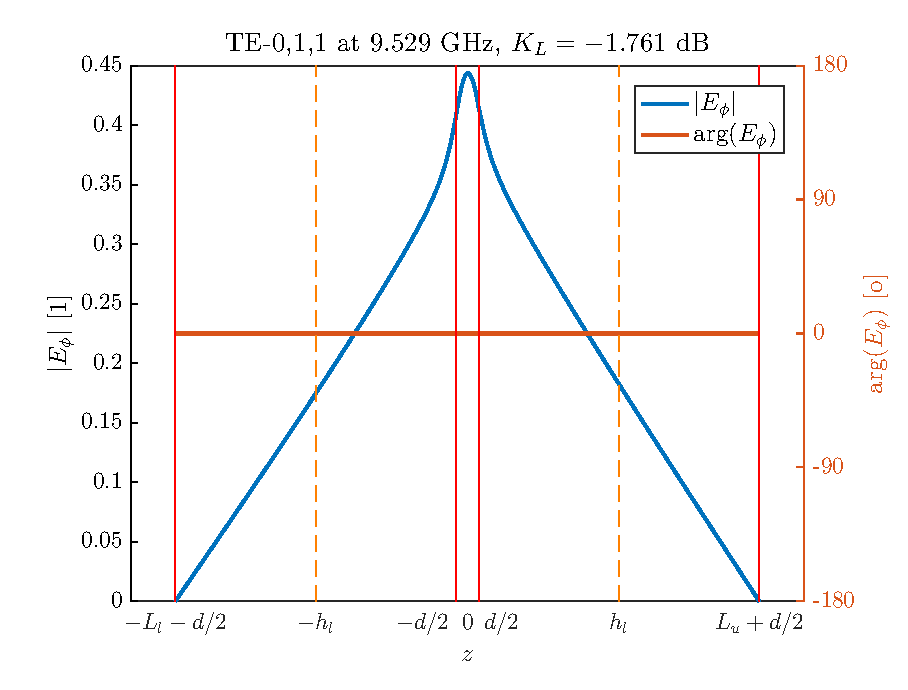
\includegraphics[width=0.8\textwidth]{mode_te011.eps}
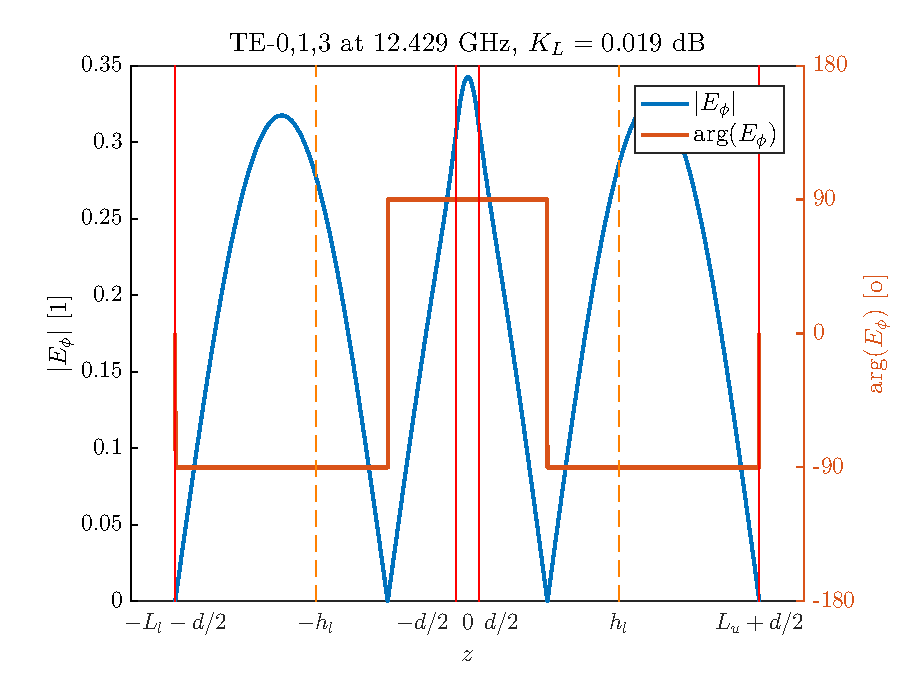
\includegraphics[width=0.8\textwidth]{mode_te013.eps}
\end{figure}

\begin{figure}
\centering
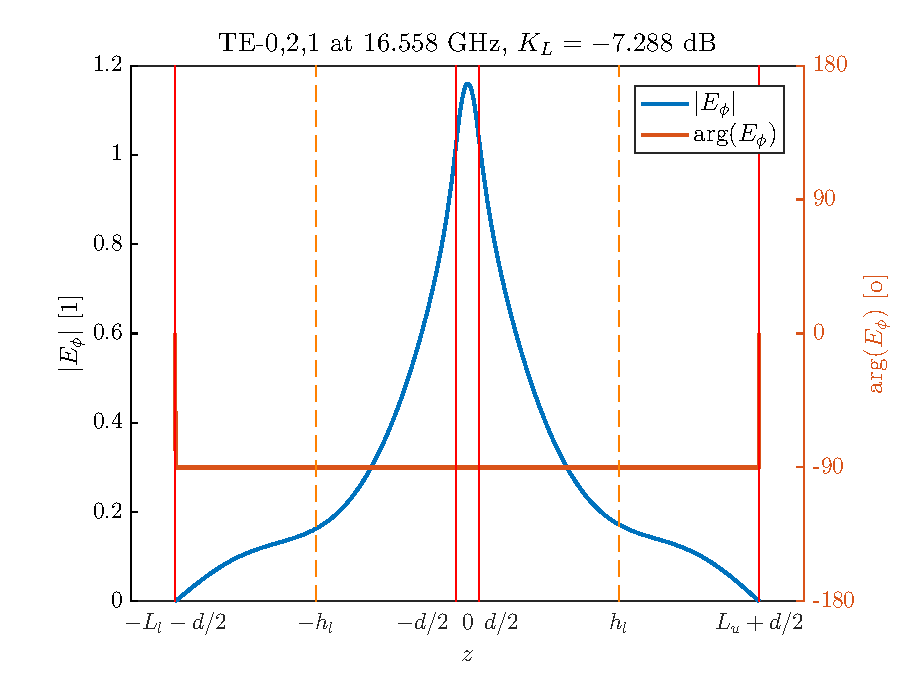
\includegraphics[width=0.8\textwidth]{mode_te021.eps}
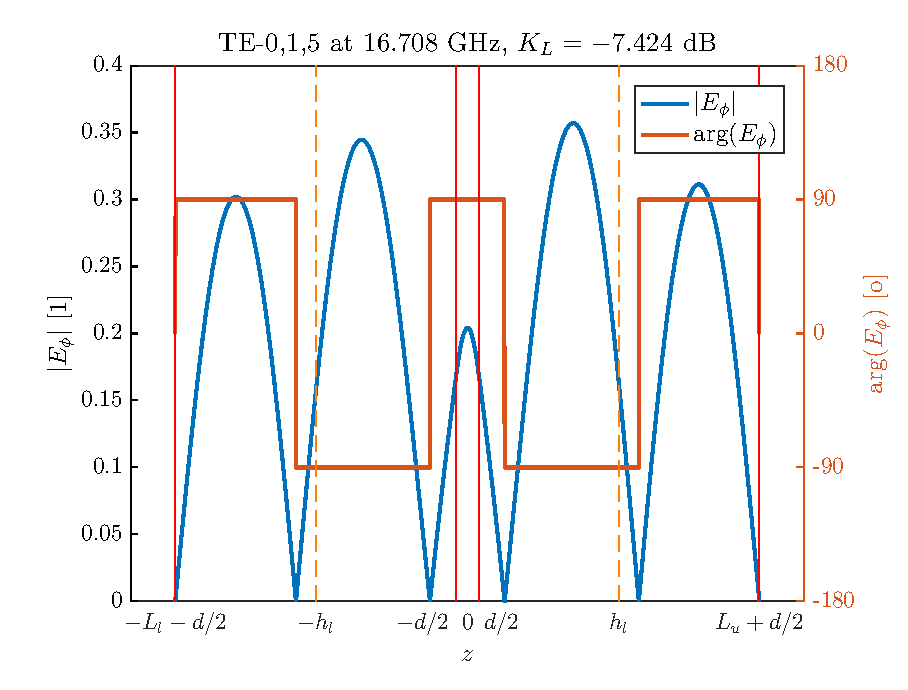
\includegraphics[width=0.8\textwidth]{mode_te015.eps}
\caption{The electric field $E_{\phi}(\rho=\frac{a_l}{2},z)$ of the first four odd TE\st{0np} modes of our split-cylinder resonator for a PTFE sample with a thickness of \SI{2}{\milli\meter}: The plot illustrates the absolute value and phase of the electric field of each mode along the z-axis. The relative permittivity of the sample $\epsilon_r$ is 2.056, the geometry of our resonator is used and 75 modes were included in the calculation. As a measure for the coupling of each mode a coupling constant $K_L=20\log(|H_{z,l}(\rho=a_l,z=h_l)|/\sqrt{4W_m/(V\mu_0)})$ is shown in the upper right corners of the plots.}\label{fig:first_modes}
\end{figure}

After this rather lengthy explanation of how to find and compute the modes of the split-cylinder resonator, we would like to include an example of a field calculation with our model to give the reader a useful insight into the method. It should also allow him to compare his implementation of the software to ours. As an example we computed the resonant frequencies of the first nine TE\st{0np} modes of our split-cylinder prototype for a PTFE sample. The sample had a thickness of \SI{2}{\milli\meter} and a relative permittivity $\epsilon_r$ of 2.056. We included 75 modes in the eigenmode expansion of the lower and upper cavity, as well as the right amount of modes in the specimen region to have optimum relative convergence. The nine modes included five odd TE\st{0np} modes, i.e. modes with an odd mode index $p$, and four even modes, i.e. modes with an even mode index $p$. Table \ref{tb:modes} lists the resonant frequencies and dominant modes of these first nine modes. Unlike Janezic's symmetric split-cylinder model, our asymmetric split-cylinder model also computes the even modes. These modes are in general not suitable for measurements, since the electric field vector of these modes has a minimum in the specimen region. This makes the fields of the modes less sensitive to the permittivity of the specimen and reduces the dielectric loss. While the former is less of a problem due to the high accuracy of our permittivity measurements, the latter reduces the accuracy of our dielectric measurements for low-loss dielectrics. Out of this reason, we usually also prefer the odd TE\st{0np} for complex permittivity measurements. In Fig. \ref{fig:first_modes} the electric field of the first four odd modes of our split-cylinder resonator for the PTFE sample is illustrated. As expected the electric field has a local maximum in the center of the substrate region. Apart from the electric field strength in the sample, Fig. \ref{fig:first_modes} also marks the location of the coupling loops in the cavity. Since the $z$ component of the magnetic field $H_z$ has the same minima along the z-axis as the electric field, the plot also illustrates the strength of the coupling of each mode.
\begin{table}
\centering
\begin{tabular}{|c|c|}
\hline\rule{0pt}{2.6ex}
Resonant frequency $f_r$ (\si{\giga\hertz}) & Mode \\
\hline\rule{0pt}{2.6ex}
 9.529 & TE\st{011} \\
11.178 & TE\st{012} \\
12.429 & TE\st{013} \\
14.970 & TE\st{014} \\
16.558 & TE\st{021} \\
16.708 & TE\st{015} \\
18.463 & TE\st{022} \\
18.959 & TE\st{023} \\
19.719 & TE\st{016} \\
\hline
\end{tabular}
\caption{Modes of our split-cylinder resonator from \SIrange{0.1}{20}{\giga\hertz} for a PTFE sample with a thickness of \SI{2}{\milli\meter}. The relative permittivity of the sample $\epsilon_r$ is 2.056, the geometry of our resonator is used and 75 modes were included in the calculation.}\label{tb:modes}
\end{table}
\section{Losses of the Measurement Model}\label{sec:losses}
As mentioned in the last chapter on the fields of the measurement model, the dielectric losses of the sample and the conductor losses of the cavity were neglected in the derivation of the field configuration of the resonator. It was acknowledged that these losses generally have a negligible influence on the fields in the cavity and that they can be neglected to simplify the field calculation. To measure the loss tangent $\tan\delta$ of a sample, which together with the dielectric constant $\epsilon$ constitutes the complex permittivity $\underline{\epsilon}=\epsilon-j\epsilon\tan\delta$, the losses must be reintroduced into our calculations. This is achieved as such that the field configuration in the resonator is computed with an $\epsilon_r$ measurement, where the measured $\epsilon_r$ is obtained from a measured resonant frequency $f_r$ and thickness $d$ of the sample, or from similar measurements. Then, the losses in the cavity are re-introduced by computing the dielectric loss
\begin{equation}\label{eq:d_loss}
P_d=\frac{1}{2}\iiint\limits_{\mathit{V}}\omega\epsilon\tan\delta\,|\vec{E}|^2\mathit{dV}\text{,}
\end{equation}
and the conductor losses
\begin{equation}\label{eq:c_loss}
P_c=\frac{R_s}{2}\iint\limits_{\mathit{A}}|\vec{H}_{t}|^2\mathit{dA}\text{,}
\end{equation}
where $R_s$ is the surface resistivity of the cavity, which we will obtain through a calibration, and $\vec{H}_{t}$ is the tangential magnetic field on the conductor surface \cite{pozar}.

The loss tangent is computed from the measured unloaded quality factor
\begin{equation}
Q_0=\omega\frac{\text{Stored energy}}{\text{Power dissipated}}=\left.\frac{\omega W}{P}\right\vert_{W(\omega_r)=2W_e(\omega_r)}=\frac{2\omega W_e}{P}\text{,}
\end{equation}
which is a ratio of the stored energy $W$ of a cavity and the power dissipated $P$ in a cavity. At resonance the magnetic energy is equal to electric energy in the cavity, so the total energy can be written as two times the electric energy of a cavity. The electric energy in the cavity is the volume integral of the squared magnitude of the electric field over the entire volume of the resonator,
\begin{equation}\label{eq:energy}
W_e=\iiint\limits_{\mathit{V}}\frac{1}{4}\epsilon|\vec{E}|^2\mathit{dV}\text{.}
\end{equation}

Broken down into the individual electric energies and losses the unloaded quality factor Q of the resonator is
\begin{equation}
Q_0=\frac{2\omega(W_u+W_s+W_l)}{P_{e,u}+P_{e,l}+P_{w,u}+P_{w,l}+P_{f,u}+P_{f,l}+P_s}\text{,}
\end{equation}
where $W_u$, $W_s$ and $W_l$ are the electric energies of the upper cavity region, sample region and lower cavity region. The losses of the resonator are divided into the conductor losses of the cavities and the dielectric loss of the sample $P_s$. The conductor losses are the losses on the surface of the metallic enclosure of the resonator, which we approximated as perfect electric conductors in our field derivation. These include the losses in the end plates, $P_{e,u}$ and $P_{e,l}$, in the walls, $P_{w,u}$ and $P_{w,l}$, and in the flanges, $P_{f,u}$ and $P_{f,l}$, of the upper and lower cavities, but naturally does not include the conductive boundary along the circumference of the sample that we introduced to approximate the split-cylinder with a closed cavity.

As the numerical integrals for the energies and losses are relatively computationally expensive, we can calculate the analytical integrals of the eigenmode expansions to simplify the computations. The volume integral of the squared magnitude of an electric field\eqref{eq:energy} gives us the electric energy in the upper cavity
\begin{align}
W_u =& \frac{\epsilon_{\text{lab}} }{4}\iiint\limits_{\mathit{V}}|\vec{E}|^2 \mathit{dV}=\frac{\epsilon_{\text{lab}}}{4}\int\limits_{\frac{d}{2}}^{\frac{d}{2}+L_u}\int\limits_0^{2\pi}\int\limits_0^{a_u} E_{\phi,u}E_{\phi,u}^* \rho\mathit{d\rho d\phi dz}\\
	=& \frac{\epsilon_{\text{lab}}\pi a_u^2}{4}\sum\limits_{n=1}^{N_u}|A_nU_nJ_0(h_{n,u}a_u)|^2\left\lbrace\frac{L_u}{2}-\frac{1}{4p_{n,u}}\sin(2p_{n,u}L_u)\right\rbrace\begin{cases}-1, &p_{n,u}\in\mathbb{I}\\1, &p_{n,u}\in\mathbb{R}\end{cases}\text{,}\label{eq:w_u}
 \end{align}
the electric energy in the sample region
\begin{align}
W_s =& \frac{\epsilon_r}{4}\iiint\limits_{\mathit{V}}|\vec{E}|^2 \mathit{dV}=\frac{\epsilon_r}{4}\int\limits_{-\frac{d}{2}}^{\frac{d}{2}}\int\limits_0^{2\pi}\int\limits_0^b E_{\phi,s}E_{\phi,s}^* \rho\mathit{d\rho d\phi dz}\\
	=& \frac{\epsilon_r\pi b^2}{4}\sum\limits_{m=1}^{N_s}J_0(h_{m,s}b)^2\times\nonumber\\&\begin{cases}|B_mV_m|^2(\frac{d}{2}+\frac{1}{2p_{m,s}}\sin(2p_{m,s}\frac{d}{2}))-|C_mW_m|^2(\frac{d}{2}-\frac{1}{2p_{m,s}}\sin(2p_{m,s}\frac{d}{2})), & p_{m,s}\in\mathbb{I}\\|B_mV_m|^2(\frac{d}{2}+\frac{1}{2p_{m,s}}\sin(2p_{m,s}\frac{d}{2}))+|C_mW_m|^2(\frac{d}{2}-\frac{1}{2p_{m,s}}\sin(2p_{m,s}\frac{d}{2})), & p_{m,s}\in\mathbb{R}\end{cases}
 \end{align}
 and the electric energy in the lower cavity
 \begin{align}
W_l =& \frac{\epsilon_{\text{lab}} }{4}\iiint\limits_{\mathit{V}}|\vec{E}|^2 \mathit{dV}=\frac{\epsilon_{\text{lab}}}{4}\int\limits_{-\frac{d}{2}-L_l}^{-\frac{d}{2}}\int\limits_0^{2\pi}\int\limits_0^{a_l} E_{\phi,l}E_{\phi,l}^* \rho\mathit{d\rho d\phi dz}\\
	=& \frac{\epsilon_{\text{lab}}\pi a_l^2}{4}\sum\limits_{p=1}^{N_l}|D_pL_pJ_0(h_{p,l}a_l)|^2\left\lbrace\frac{L_l}{2}-\frac{1}{4p_{p,l}}\sin(2p_{p,l}L_l)\right\rbrace\begin{cases}-1, &p_{p,l}\in\mathbb{I}\\1, &p_{p,l}\in\mathbb{R}\end{cases}\text{.}\label{eq:w_l}
 \end{align}
Similarly, the surface integral of the tangential magnetic field on the cavity surface \eqref{eq:c_loss} yields the losses of the upper cavity's end plate
\begin{align}
P_{e,u}=&\frac{R_s}{2}\iint\limits_{\mathit{A}}|\vec{H}_{t}|^2\mathit{dA}=\frac{R_s}{2}\int\limits_0^{2\pi}\int\limits_0^{a_u}H_{\rho,u}H_{\rho,u}^*\left(z=\frac{d}{2}+L_u\right) \rho\mathit{d\rho d\phi}\\ =& \frac{R_s\pi a_u^2}{\omega^2 \mu_0^2 2}\sum\limits_{n=1}^{N_u}|p_{n,u}A_nU_nJ_0(h_{n,u}a_u)|^2\text{,}\label{eq:p_eu}
\end{align}
the losses of the lower cavity's end plate
\begin{align}
P_{e,l}=&\frac{R_s}{2}\iint\limits_{\mathit{A}}|\vec{H}_{t}|^2\mathit{dA}=\frac{R_s}{2}\int\limits_0^{2\pi}\int\limits_0^{a_l}H_{\rho,l}H_{\rho,l}^*\left(z=-\frac{d}{2}-L_l\right) \rho\mathit{d\rho d\phi}\\ =& \frac{R_s\pi a_l^2}{\omega^2 \mu_0^2 2}\sum\limits_{p=1}^{N_l}|p_{p,l}D_pL_pJ_0(h_{p,l}a_l)|^2\text{,}\label{eq:p_el}
\end{align}
the losses in the walls of the upper cavity
\begin{align}
P_{w,u}=&\frac{R_s}{2}\iint\limits_\mathit{A}|\vec{H}_t|^2\mathit{dA}=\frac{R_s}{2}\int\limits_{\frac{d}{2}}^{\frac{d}{2}+L_u}\int\limits_0^{2\pi}H_{z,u}H_{z,u}^*(\rho=a_u)a_u\mathit{d\phi dz}\\
       =& \frac{R_s\pi a_u}{\omega^2\mu_0^2}\sum\limits_{n=1}^{N_u}\sum\limits_{n'=1}^{N_u}A_nA_{n'}^*U_nU_{n'}^*h_{n,u}h_{n',u}J_0(h_{n,u}a_u)J_0(h_{n',u}a_u)\times\nonumber\\&
       \begin{cases}
        	-\frac{1}{2}L_u+\frac{1}{4p_{n,u}}\sin(2p_{n,u}L_u), &(n=n') \wedge (p_{n,u}\in\mathbb{I})\\
        	 \frac{1}{2}L_u-\frac{1}{4p_{n,u}}\sin(2p_{n,u}L_u), &(n=n')  \wedge  (p_{n,u}\in\mathbb{R})\\
        	 \frac{\sin\left(\left(p_{n,u}-p_{n',u}\right)L_u\right)}{2\left(p_{n,u}-p_{n',u}^*\right)}-\frac{\sin\left(\left(p_{n,u}+p_{n',u}^*\right)L_u\right)}{2\left(p_{n,u}+p_{n',u}^*\right)}, &(n\neq n')
       \end{cases}\text{,}\label{eq:p_wu}
\end{align}
the losses in the walls of the lower cavity
\begin{align}
P_{w,l}=&\frac{R_s}{2}\iint\limits_\mathit{A}|\vec{H}_t|^2\mathit{dA}=\frac{R_s}{2}\int\limits_{-\frac{d}{2}-L_l}^{-\frac{d}{2}}\int\limits_0^{2\pi}H_{z,l}H_{z,l}^*(\rho=a_l)a_l\mathit{d\phi dz}\\
       =& \frac{R_s\pi a_l}{\omega^2\mu_0^2}\sum\limits_{p=1}^{N_l}\sum\limits_{p'=1}^{N_l}D_pD_{p'}^*L_pL_{p'}^*h_{p,l}h_{p',l}J_0(h_{p,l}a_l)J_0(h_{p',l}a_l)\times\nonumber\\&
       \begin{cases}
        	-\frac{1}{2}L_l+\frac{1}{4p_{p,l}}\sin(2p_{p,l}L_l), &(p=p') \wedge (p_{p,l}\in\mathbb{I})\\
        	 \frac{1}{2}L_l-\frac{1}{4p_{p,l}}\sin(2p_{p,l}L_l), &(p=p')  \wedge  (p_{p,l}\in\mathbb{R})\\
        	 \frac{\sin\left(\left(p_{p,l}-p_{p',l}\right)L_l\right)}{2\left(p_{p,l}-p_{p',l}^*\right)}-\frac{\sin\left(\left(p_{p,l}+p_{p',l}^*\right)L_l\right)}{2\left(p_{p,l}+p_{p',l}^*\right)}, &(p\neq p')
       \end{cases}\text{,}\label{eq:p_wl}
\end{align}
the losses on the flange of the upper cavity
\begin{align}
P_{f,u}=&\frac{R_s}{2}\iint\limits_\mathit{A}|\vec{H}_t|^2\mathit{dA}=\frac{R_s}{2}\int\limits_0^{2\pi}\int\limits_{a_u}^b H_{\rho,s}H_{\rho,s}^*\left(z=\frac{d}{2}\right)\rho \mathit{d\rho d\phi}\\
=& \frac{R_s\pi}{\omega^2\mu_0^2}\sum\limits_{m=1}^{N_s}\sum\limits_{m'=1}^{N_s}p_{m,s}p_{m',s}^* 
 \left\lbrace -B_mV_m\sin(p_{m,s}\frac{d}{2})+C_mW_m\cos(p_{m,s}\frac{d}{2})\right\rbrace\times\nonumber\\
 &\left\lbrace -B_{m'}V_{m'}\sin(p_{m',s}\frac{d}{2})+C_{m'}W_{m'}\cos(p_{m',s}\frac{d}{2})\right\rbrace^*\times\\\label{eq:p_fu}
 &\begin{cases}
 \frac{b^2}{2}J_0^2(h_{m,s}b)-\frac{a_u^2}{2}(J_0^2(h_{m,s}a_u)+J_1^2(h_{m,s}a_u))+\frac{a_u}{h_{m,s}}J_0(h_{m,s}a_u)J_1(h_{m,s}a_u),& m=m'\\
 -\frac{a_u}{h_{m,s}^2-h_{m',s}^2}(h_{m',s}J_1(h_{m,s}a_u)J_0(h_{m',s}a_u)-h_{m,s}J_0(h_{m,s}a_u)J_1(h_{m',s}a_u)),& m\neq m'
 \end{cases}\text{,}\nonumber
\end{align}
and the losses on the flange of the lower cavity
\begin{align}
P_{f,l}=&\frac{R_s}{2}\iint\limits_\mathit{A}|\vec{H}_t|^2\mathit{dA}=\frac{R_s}{2}\int\limits_0^{2\pi}\int\limits_{a_l}^b H_{\rho,s}H_{\rho,s}^*\left(z=-\frac{d}{2}\right)\rho \mathit{d\rho d\phi}\\
=& \frac{R_s\pi}{\omega^2\mu_0^2}\sum\limits_{m=1}^{N_s}\sum\limits_{m'=1}^{N_s}p_{m,s}p_{m',s}^* 
 \left\lbrace B_mV_m\sin(p_{m,s}\frac{d}{2})+C_mW_m\cos(p_{m,s}\frac{d}{2})\right\rbrace\times\nonumber\\
 &\left\lbrace B_{m'}V_{m'}\sin(p_{m',s}\frac{d}{2})+C_{m'}W_{m'}\cos(p_{m',s}\frac{d}{2})\right\rbrace^*\times\\
 &\begin{cases}
 \frac{b^2}{2}J_0^2(h_{m,s}b)-\frac{a_l^2}{2}(J_0^2(h_{m,s}a_l)+J_1^2(h_{m,s}a_l))+\frac{a_l}{h_{m,s}}J_0(h_{m,s}a_l)J_1(h_{m,s}a_l),& m=m'\\
 -\frac{a_l}{h_{m,s}^2-h_{m',s}^2}(h_{m',s}J_1(h_{m,s}a_l)J_0(h_{m',s}a_l)-h_{m,s}J_0(h_{m,s}a_l)J_1(h_{m',s}a_l)),& m\neq m'
 \end{cases}\text{.}\nonumber
\end{align}
Finally, the volume integral over the electric field \eqref{eq:d_loss} in the sample region leads to the dielectric loss of the sample
\begin{align}
P_s=&\frac{1}{2}\iiint\limits_{\mathit{V}}\omega\epsilon\tan\delta\,|\vec{E}|^2\mathit{dV}
   =\frac{\omega\epsilon'\tan\delta}{2}\int\limits_0^{2\pi}\int\limits_{-\frac{d}{2}}^{\frac{d}{2}}\int\limits_0^bE_{\phi,s}E_{\phi,s}^*\rho \mathit{d\rho dz d\phi}\nonumber\\
   =&\frac{\omega\epsilon_r\pi b^2\tan\delta}{2}\sum\limits_{m=1}^{N_s}J_0^2(h_{m,s}b)\times\\
   &\begin{cases}
   |B_mV_m|^2\left(\frac{d}{2}+\frac{1}{2p_{m,s}}\sin\left(2p_{m,s}\frac{d}{2}\right)\right)-|C_mW_m|^2\left(\frac{d}{2}-\frac{1}{2p_{m,s}}\sin\left(2p_{m,s}\frac{d}{2}\right)\right), & p_{m,s}\in \mathbb{I} \\
   |B_mV_m|^2\left(\frac{d}{2}+\frac{1}{2p_{m,s}}\sin\left(2p_{m,s}\frac{d}{2}\right)\right)+|C_mW_m|^2\left(\frac{d}{2}-\frac{1}{2p_{m,s}}\sin\left(2p_{m,s}\frac{d}{2}\right)\right), & p_{m,s}\in \mathbb{R}
   \end{cases}\text{.}\nonumber
\end{align}
The dielectric loss of the sample is proportional to the loss tangent $\tan\delta$. If we calculate the dielectric loss by subtracting the conductor losses from the total measured losses $P=\frac{2\omega W_e}{Q_0}$, we easily obtain the loss tangent
\begin{align}\label{eq:tand}
\tan\delta=\left(\frac{2\omega(W_u+W_s+W_l)}{Q_0}-P_{e,u}-P_{e,l}-P_{w,u}-P_{w,l}-P_{f,u}-P_{f,l}\right)/P_s'\text{,}
\end{align}
where $P_s'=P_s/\tan\delta$ is the normalised dielectric loss.
\subsection{Example of a Complex Permittivity Measurement Carried out with the M12 Model}\label{ss:ptfe}
Now that we have derived the entire M12 model we think the reader might benefit from an example of a complex permittivity measurement with the model. We only cover the calibration and the convergence of the model in the upcoming sections, so all the necessary theory is already available to us. In this example we are going to measure a PTFE sample with a thickness of \SI{1.509}{\milli\meter} with the TE\st{011} mode of the split-cylinder prototype. We begin with finding the TE\st{011} mode of the resonator: As we have already mentioned, the TE\st{011} mode is not the fundamental mode of the resonator and to complicate things even more the mode order in the split-cylinder depends on the dielectric constant of the specimen. Although coupling loops suppress the TM mode in the resonator, a number of TE modes still exist in the resonator making mode identification hard. An \er{} estimate is necessary to find the \te{} mode. This \er{} estimate may be a measurement with another method (e.g. a capacitance method), measurement data from a data sheet, or as suggested by Janezic \cite{janezicarz} an \er{} estimate from the fundamental TE\st{111} mode of the split-cylinder. It turns out that a simple split-cylinder model with a uniform diameter gives a reasonably accurate estimate of \er{}. We measured the transmission coefficient of the resonator of the fundamental mode (i.e. the first peak of the transmission coefficient) in the lab, which had its peak at \SI{5.2748}{\giga\hertz}. For this resonant frequency the model gives us an estimated \er{} of around 2.0815.
\begin{figure}
\centering
\begin{tikzpicture}
	\begin{axis}[	scale only axis,
					height=0.25\textheight,
					scaled x ticks=base 10:-9,
					xtick distance=0.05e9,
					xmin=9.53e9,
					xmax=9.774e9,
					xlabel={$f$ [\si{\hertz}]},
					ylabel={$20\log_{10}|S_{21}|$ [\si{\decibel}]},
					ymin=-100,
					ymax=-50]
		\addplot[blue] table[	col sep=comma,
								mark=none,
								x index=0,
								y index=1,
								header=false] {figures/PTFE_sample.csv};
		\node[pin=90:$TE_{011}$] at (9.6614e+09,-65.8523) {};		
	\end{axis}
\end{tikzpicture}
\caption{Resonance curve of the TE\st{011} mode of our split-cylinder prototype loaded with a \SI{1.509}{\milli\meter} thick PTFE sample. The resonant frequency of the mode was \SI{9.6619}{\giga\hertz} and the quality factor factor was \num{8754.3}, which both were obtained through a circle-fit of the resonance curve.}\label{fig:rc_ptfe}
\end{figure}

With this estimate for the dielectric constant \er{} we can now estimate the resonant frequency of the \te mode using the M12 model. For this we calculate the roots of the determinant 
\begin{equation}
\det(\mat{Z}(f,\epsilon_r=2.0815,d=\SI{1.509}{\milli\meter}))=0
\end{equation}
for the \er-estimate 2.0815 and the measured thickness of the sample $d=\SI{1.509}{\milli\meter}$. The first root at \SI{9.653}{\giga\hertz} is the estimated resonant frequency of the \te mode for the dielectric constant estimate and measured thickness. As the dielectric constant of low-dielectrics typically varies slowly with frequency the estimate should lie very closely to the true resonant frequency of the \te mode. Next, we need to measure the transmission coefficient around the resonant frequency estimate to find this true resonant frequency. Fig. \ref{fig:rc_ptfe} illustrates a measurement of the transmission coefficient that we performed around the estimate. To minimize the influence of the coupling network on this measurement we used very loose coupling. As there was only one resonance curve close to our estimate, the quality factor measurement of the curve gave us the resonant frequency \SI{9.6619}{\giga\hertz} and the quality factor \num{8754.3} of the \te mode. Our model allows us to compute the dielectric constant of our sample for this frequency by finding the first root of
\begin{equation}
\det(\mat{Z}(f=\SI{9.6619}{\giga\hertz},\epsilon_r,d=\SI{1.509}{\milli\meter}))=0\text{.}
\end{equation}
The first root and the dielectric constant of the sample is $\epsilon_r=2.0563$, for which the field configuration is shown in Fig. \ref{fig:mode_ptfe}. Lastly, we can use the solution of this measurement to calculate the \tand{} with Equation \eqref{eq:tand} from the surface resistance $R_s$ of the resonator and the measured quality factor $Q$ of the mode. The result of the equation is the loss tangent $\tan\delta=\num{2.2208e-4}$.
\begin{figure}
\centering
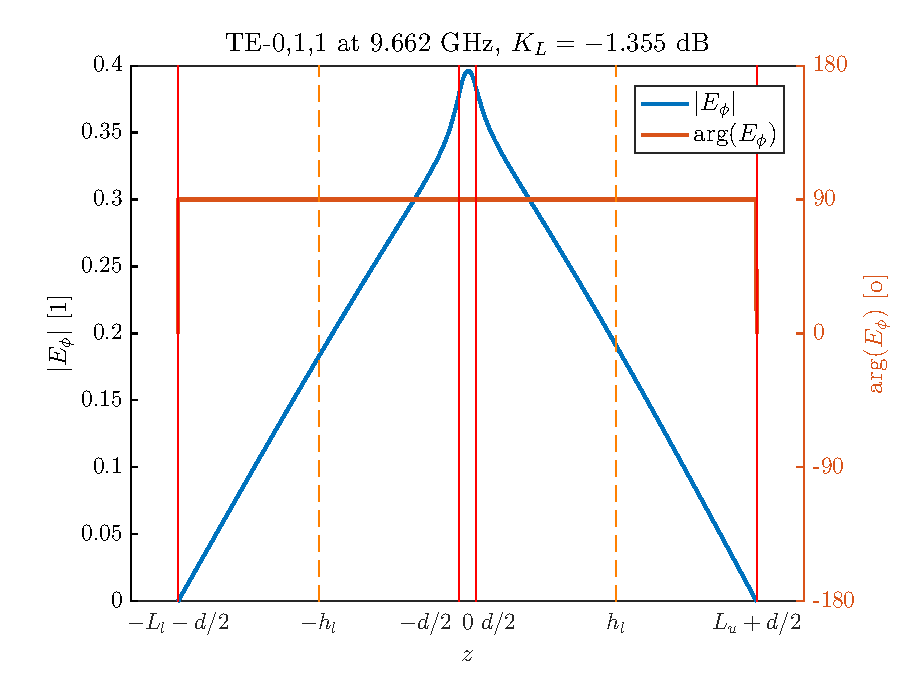
\includegraphics[height=0.3\textheight]{PTFE_sample.eps}
\caption{The electric field $E_{\phi}(\rho=\frac{a_l}{2},z)$ of the TE\st{011} mode of the sample along the z-axis of the split-cylinder. The sample was a \SI{1.509}{\milli\meter} thick PTFE sample with a dielectric constant $\epsilon$ of \num{2.0563}. The plot also indicates the boundaries of the resonator and the location of the coupling loops. As a measure for the coupling of the mode a coupling constant $K_L$ is shown in the upper right corner of the plot.}\label{fig:mode_ptfe}
\end{figure}
\section{Fields of the Calibration Model}
\begin{figure}
\centering
\begin{tikzpicture}
   %\draw[step=1cm,gray,very thin] (0,0) grid (8,7);
    \node[anchor=south west,inner sep=0] (image) at (0,0) {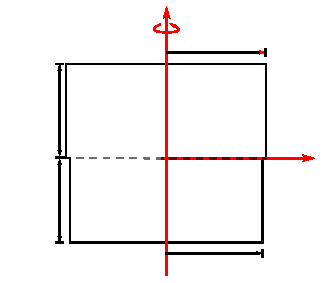
\includegraphics[width=8cm]{split_cylinder_resonator_cal_model.pdf}};
    \draw (4,6.9) node[red] {\textit{z}};
    \draw (7.75,3) node[red] {\textit{$\rho$}};
    \draw (1,4.1) node {$L_u$};
    \draw (1,2) node {$L_l$};
    \draw (5.2,5.85) node {$a_u$};
    \draw (5.2,0.4) node {$a_l$};
    
    \draw (2.4,2) node[anchor=west] {\scalebox{0.75}{$\mu_0,\epsilon_{lab}$}};
    \draw (2.4,4.10) node[anchor=west]  {\scalebox{0.75}{$\mu_0,\epsilon_{lab}$}};
\end{tikzpicture}
\caption{Geometry of the asymmetric split-cylinder's calibration model.}\label{fig:cal_model}
\end{figure}
In the previous sections we have taken a closer look at the M12 model, which we developed and tested during the course of these sections. We also recognised that the M12 model used a large number of variables to compute the modes of the resonator and that therefore the accuracy of the model relied on the accuracy of these variables. Like for any physical model the actual measurement variables and the setup of the resonator must closely resemble the measurement variables and the geometry of the model. Unfortunately, this model has a few systematic errors that are not part of the model and that disturb our measurements. During our measurements we identified a few potential sources of systematic error, which include:
\begin{itemize}
\item Geometry of the cavities (Taper of the cylindrical cavities, parallelism and flatness of the cylinder faces, ...)
\item Properties of the setup (Eccentricity of the two half-cylinders, unequal surface losses due to surface finish variations, dust and dirt)
\item Properties of the sample (Compression of the sample, geometry of the sample (flatness, parallelism), impurities)
\end{itemize}
Although these systematic errors cannot be avoided altogether, there are strategies to minimise these uncertainties. One strategy is an error correction based on a calibration. In such a strategy a calibration standard is measured and using a reference value for the calibration standard the measurement model is adjusted to zero out the difference between the measured value and the reference value. Janezic \cite{janezic} included a calibration procedure in his split-cylinder model that involved a measurement of the empty split-cylinder resonator. In this procedure the dielectric sample is removed from the resonator and both half-cavities are pressed together without a sample in between. The symmetric split-cylinder is turned into a cylindrical cavity! Then, the resonance curve of the TE\st{011} mode is measured and the result of the measurement is used to adjust the radius $a$ and the conductivity $\sigma$ of resonator. While both compensate for the systematic errors in the measurement, the radius $a$ predominantly compensates for variations in the geometry of the setup and the conductivity $\sigma$ for the variations in the surface finish. With the conductivity $\sigma$ of the calibration we also obtain the surface resistance $R_s$ of the resonator, which is a necessary variable for the calculation of the loss tangent $\tan\delta$. This is a very important parameter of the calibration as the surface conductivity differs largely from the bulk conductivity. The surface conductivity also depends on parameters like surface roughness or contaminants, which can reduce the conductivity by more than \SI{50}{\percent} compared to the bulk conductivity. This makes the calibration of the conductivity $\sigma$ absolutely vital to accurate loss tangent measurements.

As the M12 model is based on Janezic's mode-matching model, we also decided to use a calibration for the M12 model. Like in Janezic's model the resonator is calibrated by pressing the two half-cavities together. This makes an asymmetric closed cavity out of our asymmetric split cylinder, which is not a cylindrical cavity like in Janezic's model. Out of this reason we developed a second mode-matching model exclusively for the calibration, which uses the radius of the lower cavity $a_l$ and the conductivity $\sigma$ as calibrations parameters. Even though our model uses the same calibration as Janezic's, we added a broadband calibration feature to our model. While Janezic's model only used the TE\st{011} mode for its calibration, we decided to use all available modes in our calibration. We recognised that the systematic errors of the measurements varied with each mode and that the calibration for another mode gave different results for the parameters $a_l$ and $\sigma$. We assumed that this behaviour was due to fact that the different field configurations of the modes emphasize different systematic errors. The conductivity of the resonator, for example, may vary with the different distributions of the magnetic fields on the surface of the cavity, since a lossy surface can lie in a region with high field strength for one mode and can lie in a low point for another. In our measurements we observed that the broadband calibration generally improved the measurement accuracy of higher TE\st{0np} modes of the resonator.

The derivation of our calibration model is very similar to the derivation of the M12 model. This is not very surprising, since the boundary value problem is identical to the original model, if we let the thickness of the sample become zero $d\rightarrow 0$. Although the boundary value problem is identical, we still need to match the modes at the new interface to find a solution. To do this we first take the solutions of the boundary value problem of the cylindrical waveguide of the upper cavity \eqref{eq:e_u}\eqref{eq:h_u}
\begin{align}
E_{\phi,u}(\rho,z)&=\sum\limits_{n=1}^{\infty} A_nU_nJ_1(h_{n,u}\rho)\sin(p_{n,u}\left(L_u-z\right)), &\scriptstyle (0\leq\rho\leq a_u)\wedge\left(0\leq z\leq L_u\right)\label{eq:e_uc}\\
H_{\rho,u}(\rho,z)&=\sum\limits_{n=1}^{\infty}\frac{-p_{n,u}}{j\omega\mu_0}A_nU_nJ_1(h_{nu}\rho)\cos(p_{n,u}\left(L_u-z\right)),&\scriptstyle\left(0\leq\rho\leq  a_u\right)\wedge\left(0\leq z\leq L_u\right)\label{eq:h_uc}\\
H_{z,u}(\rho,z)&=\frac{-1}{j\omega\mu_0}\sum\limits_{n=1}^\infty A_nU_nh_{n,u}J_0(h_{n,u}\rho)\sin(p_{n,u}\left(L_u-z\right)),&\scriptstyle(0\leq\rho\leq a_u)\wedge\left(0\leq z\leq L_u\right)
\end{align}
and the lower cavity \eqref{eq:e_l}\eqref{eq:h_l}
\begin{align}
E_{\phi,l}(\rho,z)&=\sum\limits_{p=1}^{\infty} D_pL_pJ_1(h_{p,l}\rho)\sin(p_{p,l}\left(z+L_l\right)), & \scriptstyle(0\leq\rho\leq a_l)\wedge\left(-L_l\leq z\leq 0\right)\label{eq:e_lc}\\
H_{\rho,l}(\rho,z)&=\sum\limits_{p=1}^{\infty}\frac{p_{p,l}}{j\omega\mu_0}D_pL_pJ_1(h_{p,l}\rho)\cos(p_{p,l}\left(z+L_l\right)), &\scriptstyle(0\leq\rho\leq a_l)\wedge\left(-L_l\leq z\leq 0\right)\label{eq:h_lc}\\
H_{z,l}(\rho,z)&=\frac{-1}{j\omega\mu_0}\sum\limits_{p=1}^\infty D_pL_ph_{p,l}J_0(h_{p,l}\rho)\sin(p_{p,l}\left(z+L_l\right)), &\scriptstyle(0\leq\rho\leq a_l)\wedge\left(-L_l\leq z\leq 0\right)\text{.}
\end{align}
As can be seen in Fig. \ref{fig:cal_model}, we only have one interface at $z=0$ in this boundary value problem, where need to match the eigenmode expansions of the fields in the cavity. Like for the M12 model, the mode matching at the interface solves the boundary value problem of the TE\st{0np} modes. The first boundary condition is the continuity of the tangential electric field
\begin{align}\label{eq:bcc_1}
E_{\phi,u}\left(\rho,z=0\right)= \begin{cases}
    E_{\phi,l}(\rho,z=0) , & 0\leq\rho\leq a_l\\
    0, & a_l\leq\rho\leq a_u
  \end{cases}\text{,}
\end{align}
which matches the electric field of the upper cavity to that of the lower cavity at the interface. Like in the previous derivations, we again insert the fields \eqref{eq:e_uc}\eqref{eq:e_lc} into the boundary condition and compute the scalar product of the tangential electric field and $H_{\rho,u}^{(n)}$ on each side of the equation. Since only the first-order Bessel function of the first kind $J_1(h_{n,u}\rho)$ of $H_{\rho,u}^{(n)}$ varies with $\rho$, we can compute
\begin{equation}
\begin{split}
\int\limits_0^{2\pi}\int\limits_0^{a_u}\sum\limits_{n'=1}^\infty A_{n'}U_{n'}J_1(h_{n',u}\rho)\sin(p_{n',u}L_u)J_1(h_{n,u}\rho)\rho\mathit{d\rho d\phi}\\=\int\limits_0^{2\pi}\int\limits_0^{a_l}\sum\limits_{p=1}^\infty D_{p}L_{p}J_1(h_{p,l}\rho)\sin(p_{p,l}L_l)J_1(h_{n,u}\rho)\rho\mathit{d\rho d\phi}
\end{split}\text{.}
\end{equation}
With help from the orthogonality relation of \eqref{eq:o_u}, we can compute the result of the integral, the mode-matching equation of the electric field
\begin{equation}\label{eq:c_mm_e}
A_nU_n\sin(p_{n,u}L_u)\frac{a_u^2}{2}J_0^2(h_{n,u}a_u)=\sum\limits_{p=1}^\infty D_pL_p\sin(p_{p,l}L_l)\frac{-h_{p,l}a_l}{h_{p,l}^2-h_{n,u}^2}J_0(h_{p,l}a_l)J_1(h_{n,u}a_l)\text{.}
\end{equation}

The second boundary condition is the continuity of the tangential magnetic field \eqref{eq:bcc_2} at the interface. We demand that the $\rho$ component of the magnetic field must be continuous over the entire surface of the boundary at $z=0$.
\begin{equation}\label{eq:bcc_2}
H_{\rho,u}\left(\rho,z=0\right)= H_{\rho,l}\left(\rho,z=0\right),\qquad 0\leq\rho\leq a_l
\end{equation}
Again, we enforce the boundary condition by matching the modes at the interface. Hence, we insert the eigenmode expansions of the magnetic fields \eqref{eq:h_uc}\eqref{eq:h_lc} into the boundary condition and calculate the scalar product of the tangential magnetic fields and $E_{\phi,l}^{(p)}$. This scalar product is an integral of the product of the expansion and the mode $E_{\phi,l}^{(p)}$ over the surface of the boundary
\begin{equation}
\begin{split}
\int\limits_0^{2\pi}\int\limits_0^{a_l}\sum\limits_{n=1}^\infty \frac{-p_{n,u}}{j\omega\mu_0}A_{n}U_{n}J_1(h_{n,u}\rho)\cos(p_{n,u}L_u)J_1(h_{p,l}\rho)\rho\mathit{d\rho d\phi}\\=\int\limits_0^{2\pi}\int\limits_0^{a_l}\sum\limits_{p'=1}^\infty \frac{p_{p',l}}{j\omega\mu_0}D_{p'}L_{p'}J_1(h_{p',l}\rho)\cos(p_{p',l}L_l)J_1(h_{p,l}\rho)\rho\mathit{d\rho d\phi}
\end{split}\text{,}
\end{equation}
where we once more use the Bessel function instead of the whole field. If we employ the orthogonality relation of the lower cavity \eqref{eq:o_l}, the result is the mode-matching equation of the magnetic field
\begin{equation}\label{eq:c_mm_h}
\sum\limits_{n=1}^\infty A_nU_n\frac{a_lh_{p,l}p_{n,u}}{h_{p,l}^2-h_{n,u}^2}J_0(h_{p,l}a_l)J_1(h_{n,u}a_l)\cos(p_{n,u}L_u)=D_pL_p\frac{a_l^2}{2}p_{p,l}J_0^2(h_{p,l}a_l)\cos(p_{p,l}L_l)\text{.}
\end{equation}
With the two mode-matching equations at hand we can now solve the boundary value problem of the calibration. If we limit the number of modes of the eigen-mode expansions of the mode-matching equations \eqref{eq:c_mm_e} and \eqref{eq:c_mm_h} to $N_u$ modes for the upper cavity and $N_l$ modes for the lower cavity, each infinite series of the mode-matching equations becomes a finite series. Since we calculated the mode-matching equations as a scalar product of the expansion with a single mode from the upper cavity or the lower cavity, we actually get $N_s+N_l$ equations out of the two mode-matching equations. With this number of equations and the same number of unknowns the equations become a uniquely determined homogeneous system of linear equations, which we can easily solve. To simplify the notation, we can write the homogeneous system of linear equations as the matrix equation
\begin{equation}\label{eq:matZc}
\mat{Z}\vec{x}=\mat{Z}\begin{bmatrix}\vec{A}\\\vec{D}\\\end{bmatrix}=
\begin{bmatrix}
\mat{C_1}&-\mat{C_2}\\
\mat{C_3}&-\mat{C_4}\\
\end{bmatrix}\begin{bmatrix}\vec{A}\\\vec{D}\\\end{bmatrix}=
\vec{0}\text{,}
\end{equation}
where $\mat{Z}$ is the mode-matching matrix and $\vec{x}$ is a coefficient vector that contains the coefficients of the eigenmode expansion $A_n$ and $D_p$. The matrix $\mat{Z}$ contains all the equations of the mode-matching problem, which are grouped in sub-matrices $\mat{C_1}$, $\mat{C_2}$, $\mat{C_3}$ and $\mat{C_4}$. Apparently, any solution $\vec{x}$ of the matrix equation is a solution of the boundary value problem.
\begin{align}
(\mat{C_1})_{nn}&= U_n\sin(p_{n,u}L_u)\frac{a_u^2}{2}J_0^2(h_{n,u}a_u)\\
(\mat{C_2})_{np}&= L_p\sin(p_{p,l}L_l)\frac{-h_{p,l}a_l}{h_{p,l}^2-h_{n,u}^2}J_0(h_{p,l}a_l)J_1(h_{n,u}a_l)\\
(\mat{C_3})_{pn}&= U_n\frac{a_lh_{p,l}p_{n,u}}{h_{p,l}^2-h_{n,u}^2}J_0(h_{p,l}a_l)J_1(h_{n,u}a_l)\cos(p_{n,u}L_u)\\
(\mat{C_4})_{pp}&= L_p\frac{a_l^2}{2}p_{p,l}J_0^2(h_{p,l}a_l)\cos(p_{p,l}L_l)
\end{align}
Analogous to the M12 matrix, a singular matrix $\mat{Z}$ is a necessary condition for the existence of a solution of Equation \eqref{eq:matZc}. Owing to this fact, root-finding algorithms can be used to find roots of the determinant of the matrix
\begin{equation}
\det(\mat{Z}(f=f_r,a_l))=0\text{,}
\end{equation}
which for each mode used in our calibration gives a lower cavity radius $a_l$. Eventually, each lower cavity radius $a_l$ can be used a calibration parameter for the mode it was calibrated with.
\section{Losses of the Calibration Model}
The loss mechanisms of the calibration are to a large extent identical to that of the original model. We will therefore abbreviate the derivation and we will not include the integrals of the electric energy and the conductor losses, which all can be found in Section \ref{sec:losses}. The unloaded quality factor $Q_0$ is again the ratio of the electric energy to the losses in the cavity
\begin{align}
Q_0 =& \frac{2\omega(W_u+W_l)}{P_{e,u}+P_{e,l}+P_{w,u}+P_{w,l}+P_{f,u}}\\=&\frac{2\omega(W_u+W_l)}{R_s(P'_{e,u}+P'_{e,l}+P'_{w,u}+P'_{w,l}+P'_{f,u})} = \frac{2\omega(W_u+W_l)}{R_sP'}\text{,}
\end{align}
where $W_u$ and $W_l$ are the electric energy in the cavities, $P_{e,u}$ and $P_{e,l}$ are the losses in the end plates, $P_{w,u}$ and $P_{w,l}$ are the losses in the walls of the cavities, and $P_{f,l}$ is the flange loss at the interface between the two cavities. As all losses in the cavity are conductor loss we can normalize the losses and write the total loss in the cavity as the normalized loss $P'$ multiplied with the surface resistance $R_s$. Although the electric energies and losses are very similar to the ones of the M12 model, we find that it would be useful for the reader to at least list them here. The electric energy of the upper cavity was already calculated by us in \eqref{eq:w_u}
\begin{align}
W_u =& \frac{\epsilon_{\text{lab}}\pi a_u^2}{4}\sum\limits_{n=1}^{N_u}|A_nU_nJ_0(h_{n,u}a_u)|^2\left\lbrace\frac{L_u}{2}-\frac{1}{4p_{n,u}}\sin(2p_{n,u}L_u)\right\rbrace\begin{cases}-1, &p_{n,u}\in\mathbb{I}\\1, &p_{n,u}\in\mathbb{R}\end{cases}\text{,}
 \end{align}
and the electric energy of the lower cavity was calculated in \eqref{eq:w_l}
  \begin{align}
W_l =& \frac{\epsilon_{\text{lab}}\pi a_l^2}{4}\sum\limits_{p=1}^{N_l}|D_pL_pJ_0(h_{p,l}a_l)|^2\left\lbrace\frac{L_l}{2}-\frac{1}{4p_{p,l}}\sin(2p_{p,l}L_l)\right\rbrace\begin{cases}-1, &p_{p,l}\in\mathbb{I}\\1, &p_{p,l}\in\mathbb{R}\end{cases}\text{.}
 \end{align}
For the conductor losses we use our results for the losses of the upper cavity's end plate
\begin{align}
P_{e,u}=& \frac{R_s\pi a_u^2}{\omega^2 \mu_0^2 2}\sum\limits_{n=1}^{N_u}|p_{n,u}A_nU_nJ_0(h_{n,u}a_u)|^2
\end{align}
given in Equation \eqref{eq:p_eu} and the results for the losses of the lower cavity's end plate
\begin{align}
P_{e,l}=& \frac{R_s\pi a_l^2}{\omega^2 \mu_0^2 2}\sum\limits_{p=1}^{N_l}|p_{p,l}D_pL_pJ_0(h_{p,l}a_l)|^2
\end{align}
given in Equation \eqref{eq:p_el}. Next, we use our calculations of the losses in the upper cavity walls $P_{w,u}$ shown in Eq. \eqref{eq:p_wu} 
\begin{align}
P_{w,u}=& \frac{R_s\pi a_u}{\omega^2\mu_0^2}\sum\limits_{n=1}^{N_u}\sum\limits_{n'=1}^{N_u}A_nA_{n'}^*U_nU_{n'}^*h_{n,u}h_{n',u}J_0(h_{n,u}a_u)J_0(h_{n',u}a_u)\times\nonumber\\&
       \begin{cases}
        	-\frac{1}{2}L_u+\frac{1}{4p_{n,u}}\sin(2p_{n,u}L_u), &(n=n') \wedge (p_{n,u}\in\mathbb{I})\\
        	 \frac{1}{2}L_u-\frac{1}{4p_{n,u}}\sin(2p_{n,u}L_u), &(n=n')  \wedge  (p_{n,u}\in\mathbb{R})\\
        	 \frac{\sin\left(\left(p_{n,u}-p_{n',u}\right)L_u\right)}{2\left(p_{n,u}-p_{n',u}^*\right)}-\frac{\sin\left(\left(p_{n,u}+p_{n',u}^*\right)L_u\right)}{2\left(p_{n,u}+p_{n',u}^*\right)}, &(n\neq n')
       \end{cases}
\end{align}
and those of the losses in the lower cavity walls $P_{w,l}$ shown Eq. \eqref{eq:p_wl} 
\begin{align}
P_{w,l}=& \frac{R_s\pi a_l}{\omega^2\mu_0^2}\sum\limits_{p=1}^{N_l}\sum\limits_{p'=1}^{N_l}D_pD_{p'}^*L_pL_{p'}^*h_{p,l}h_{p',l}J_0(h_{p,l}a_l)J_0(h_{p',l}a_l)\times\nonumber\\&
       \begin{cases}
        	-\frac{1}{2}L_l+\frac{1}{4p_{p,l}}\sin(2p_{p,l}L_l), &(p=p') \wedge (p_{p,l}\in\mathbb{I})\\
        	 \frac{1}{2}L_l-\frac{1}{4p_{p,l}}\sin(2p_{p,l}L_l), &(p=p')  \wedge  (p_{p,l}\in\mathbb{R})\\
        	 \frac{\sin\left(\left(p_{p,l}-p_{p',l}\right)L_l\right)}{2\left(p_{p,l}-p_{p',l}^*\right)}-\frac{\sin\left(\left(p_{p,l}+p_{p',l}^*\right)L_l\right)}{2\left(p_{p,l}+p_{p',l}^*\right)}, &(p\neq p')
       \end{cases}\text{.}
\end{align}
Finally, the only remaining loss is the flange loss at the interface, which is similar to the flange loss we calculated in Eq. \eqref{eq:p_fu}.
\begin{align}
P_{f,u}=& \frac{R_s\pi}{\omega^2\mu_0^2}\sum\limits_{n=1}^{N_s}\sum\limits_{n'=1}^{N_s}p_{n,u}p_{n',u}^*A_nA_{n'}^*U_nU_{n'}^*\cos(p_{n,u}L_u)\cos(p_{n',u}L_u)^*\times\\
 &\begin{cases}
 \frac{a_u^2}{2}J_0^2(h_{n,u}a_u)-\frac{a_l^2}{2}(J_0^2(h_{n,u}a_l)+J_1^2(h_{n,u}a_l))+\frac{a_l}{h_{n,u}}J_0(h_{n,u}a_l)J_1(h_{n,u}a_l),& n=n'\\
 -\frac{a_l}{h_{n,u}^2-h_{n',u}^2}(h_{n',u}J_1(h_{n,u}a_l)J_0(h_{n',u}a_l)-h_{n,u}J_0(h_{n,u}a_l)J_1(h_{n',u}a_l)),& n\neq n'
 \end{cases}\text{,}\nonumber
\end{align}
We can then use the results for the electric energies and the conductor losses to compute the conductivity of the cavity
\begin{equation}
\sigma = \frac{\omega\mu_0}{2R_s^2}=\frac{\omega\mu_0}{2}\left(\frac{2\omega(W_u+W_l)}{Q_0P'}\right)^{-2}\text{.}
\end{equation}
This conductivity $\sigma$ is the second parameter of our calibration and allows us to calibrate the cavity for accurate loss tangent $\tan\delta$ measurements. Like the first parameter of the calibration, the lower cavity radius $a_l$, the conductivity can be calibrated not only with the TE\st{011} mode, but with multiple modes. This allows us to use different conductivities for different modes and improve the accuracy of loss tangent measurements with higher modes.
\section{Convergence of Both Models}
After we have derived both the M12 model and the calibration model for the M12 model, we still have to discuss the convergence of these mode-matching models. Although mode-matching has properties of an analytical technique, it is a numerical method and it is therefore supposed to converge to a true value with increasing numerical accuracy. We have already mentioned that mode-matching achieves this by matching the boundary condition at the interface between two field regions. In these field regions the electro-magnetic field is expanded as an infinitely long series and the mode-matching method gives an mathematically exact solution only for these infinitely long series. An exact solution is identical to a perfect match of the boundary conditions and a solution of the boundary-value problem. As an infinitely long series cannot be computed on a computer, the infinite series are truncated after a few terms and the truncated series are used to approximate the exact solution. While it is somewhat logical that the truncation of the series introduces a numerical error, a reduction of the numerical error with increasing numerical accuracy, i.e. the convergence of the mode-matching model, cannot be expected for every truncated series. It turns out that a mode-matching calculation can converge to different results depending on the number of modes used for the expansion in each region. More specifically, if the number of modes are increased equally in the regions, the result does not have to converge or converges very slowly. This phenomenon is called relative convergence and has been studied by many researchers \cite{itoh, mittra, leroy, sorrentino}. Although we could find a conclusive explanation of the phenomenon, the edge effect at boundaries \cite{mittra} and ill-conditioned equation systems \cite{leroy} were identified by others as root causes of the phenomenon. Another explanation suggested that fluctuations of one field must be supported by the modes in the other, so that the spectral content on both sides is the same.

\begin{figure}
\centering
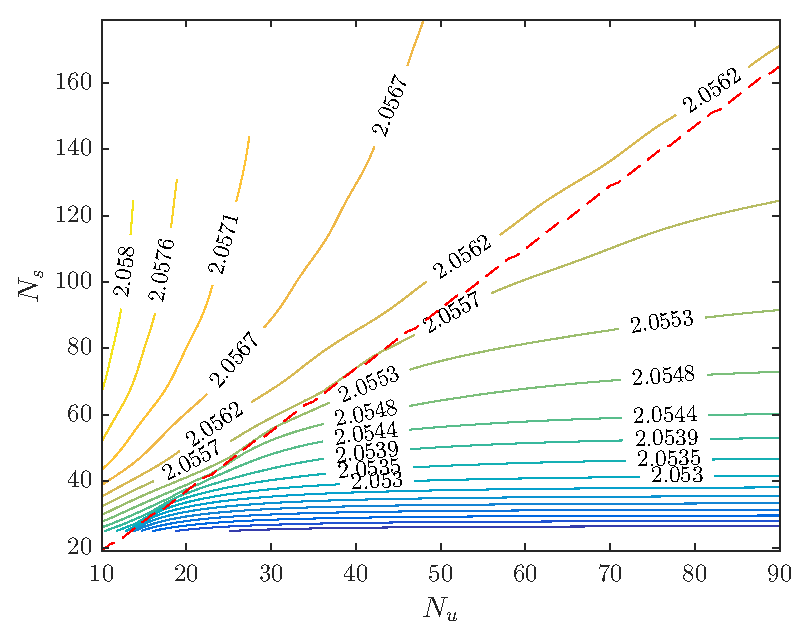
\includegraphics[scale=0.75]{RC_er.eps}
\caption{Contour plot of the relative permittivity of the PTFE sample. The permittivity is plotted against the number of modes of the sample region $N_s$ and against that of the upper cavity $N_u$. The resonant frequency used for the plot was \SI{9.6619}{\giga\hertz} and the thickness of the sample was \SI{1.509}{\milli\meter}. The dashed line shows the ideal model ratio of $N_s$ and $N_u$ according to Il'inksi \cite{ilinski} and Janezic \cite{janezic}.}\label{fig:RCer}
\end{figure}

Irrespective of the origins of the relative convergence, the relative convergence should be minimised to ensure fast convergence and low computational effort. On the one hand Janezic \cite{janezic} noted that this can be achieved by employing all available orthogonality relations. On the other hand an optimum mode ratio must be chosen for the expansions, which is the ratio of the number of modes of one region to that of another region that gives the best convergence for the computational effort spent. Different optimum mode ratios for the mode-matching method can be found in the literature. Janezic suggested with reference to an article by Il'inski \cite{ilinski} that the propagation constant $p_N$ of the highest expansion mode in each section must be equal. Earlier research used ratios of the lateral extension of two guides, but then again others found that the ratio must be chosen as such that the cut-off wave number $h_N$  is the same in each guide. As the cut-off wave number of higher modes is typically far higher than the wave number $k$, these three optimum mode ratios yield the same results for higher modes. 

\begin{figure}
\centering
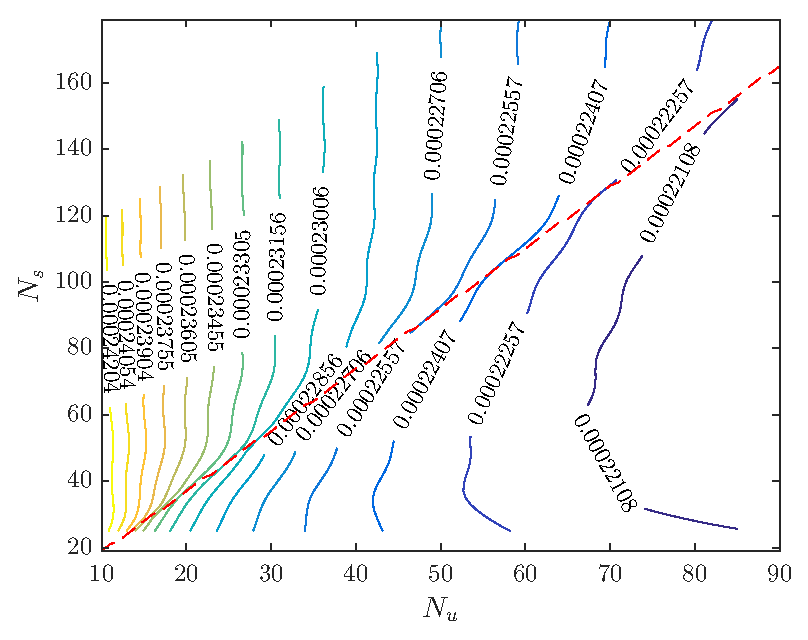
\includegraphics[scale=0.75]{RC_tand.eps}
\caption{Contour plot of the loss tangent of the PTFE sample. The loss tangent is plotted against the number of modes of the sample region $N_s$ and against that of the upper cavity $N_u$. The resonant frequency used for the plot was \SI{9.6619}{\giga\hertz}, the unloaded quality factor $Q_0$ of the resonance was \num{8754.3} and the thickness of the sample was \SI{1.509}{\milli\meter}. The dashed line shows the ideal model ratio of $N_s$ and $N_u$ according to Il'inksi \cite{ilinski} and Janezic \cite{janezic}.}\label{fig:RCtand}
\end{figure}

For the derivation of the M12 model and for that of the calibration model we naturally used all available orthogonality relations, and for our computations we also used the optimum mode ratios. To illustrate the relative convergence of the model we can plot the relative permittivity against the number of modes in the sample region and against that in the upper cavity. Again, we use the same PTFE sample that we used for most of our examples up to now, for which we measured a resonant frequency of \SI{9.6619}{\giga\hertz}, an unloaded quality factor \num{8754.3} and a thickness of \SI{1.509}{\milli\meter}. As can be seen in Fig. \ref{fig:RCer}, the convergence of the relative permittivity indeed varies with the number of modes. We also added a plot of Il'inski's optimum mode ratio to show how a mode matching model converges for an optimum mode ratio, which is marked by a dashed line in the plot. The plot exemplifies that the model converges optimally for the optimum mode ratio and that the result converges rapidly when we increase the number of modes in this ratio. It also shows that the convergence error for this ratio becomes less than \num{5e-4} for only $N_u=50$ modes. As can be seen in Fig. \ref{fig:RCtand} the relative convergence phenomenon has an influence on the loss tangent as well. As the accuracy of our loss tangent measurements is typically lower, the influence of the relative convergence on the loss tangent is less pronounced. Since our model was designed with split-cylinders in mind that have only a small difference in the geometry of their cavities, we chose $N_u=N_l$ for the computation of these plots. If we use the Il'inski optimum mode ratio for both interfaces
\begin{align}
p_{N_u,u}=p_{N_s,s} \quad\quad\quad p_{N_s,s}=p_{N_l,l}
\end{align} 
this small difference also makes $N_u$ and $N_l$ become approximately equal, $N_u\approx N_l$. For the calibration model the situation is very similar, since the variables that define the propagation constants, i.e. relative permittivity of the air in the cavities and the radii of the cavities, are equal or almost equal. Accordingly, optimum convergence of the calibration model can be achieved with the mode ratio $N_u=N_l$. Since the ideal mode ratios relate the number of modes in one region to the number of modes in the other regions, we decided to denote the number of modes in the upper cavity for a computation with an ideal mode ratio with $N=N_u$. Whenever we write $N$ for the number of modes of a split cylinder model, we actually give the number of modes in the upper cavity $N=N_u$ and all modes in the other regions through the mode ratio. 

\begin{figure}
\centering
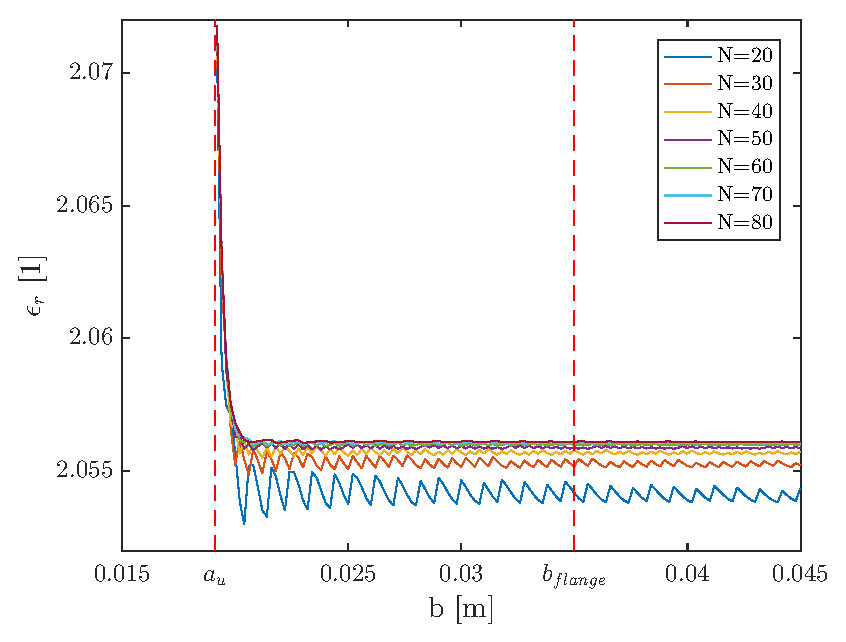
\includegraphics[scale=0.75]{b_conv_er.eps}
\caption{Convergence plot of the relative permittivity \er{} against the radius of the sample region $b$ (flange diameter). The convergence is plotted for different numbers of modes $N=20,30,40,50,60,70,80$, where $N$ refers to the number of modes in the upper cavity for optimum mode ratios (i.e. for optimum relative convergence). The resonant frequency used for the plot was \SI{9.6619}{\giga\hertz} and the thickness of the sample was \SI{1.509}{\milli\meter}. The upper cavity radius $a_u$ and the flange radius radius b\st{flange} are both marked with dashed vertical lines.}\label{fig:b_er}
\end{figure}

As shown above we can deal with the relative convergence phenomenon and ensure good convergence by choosing an optimum mode ratio for both models. But this on its own does not guarantee an accurate measurement, since the model must accurately model the field configuration in the split cylinder resonator. In Section \ref{sec:modelling} we have learnt that the split cylinder can be modelled as a closed cavity for certain modes like the TE\st{0np} modes, although it is in fact an open cavity. The region around the sample is a filled cylindrical cavity, which has a diameter of $2b$ and a length $d$. The fields in the gap of the open split-cylinder can be approximated with this filled cavity as long as we choose a diameter $2b$ that is large enough. For large diameters the electro-magnetic field in the sample region, measured at increasing distance from the origin, decays rapidly. So much, that for a certain diameter the conductive boundary at $\rho=b$ has no noticeable influence on the measurement any more. A plot of the dielectric constant (Fig. \ref{fig:b_er}) and the loss tangent (Fig. \ref{fig:b_tand}) against the radius of the sample region $b$ clearly shows that both converge rapidly if we increase the radius. If we vary the number of modes included in this computation, we can see that the convergence improves for increasing numbers of modes. Additionally, more modes also reduce the ripple of both the relative permittivity and the loss tangent. In this example, which is again our well-known PTFE sample, the relative permittivity and the loss tangent showed a ripple of around \num{2e-4} and \num{3.5e-7} for $N=30$ modes. For the number of modes that we used for most of our calculations $N=75$, the ripple became smaller than the uncertainties associated with the relative permittivity and the loss tangent. The ripple of the dielectric constant and loss tangent fell to \num{2.6e-5} and \num{1.2e-7}. These figures also show that the complex permittivity becomes stationary for $b>\SI{25}{\milli\meter}$, so we can choose any $b$ larger than \SI{25}{\milli\meter} without introducing any major error. Obviously, $b>\SI{25}{\milli\meter}$ yields a sufficiently accurate approximation of an open cavity for these two parameters. This does not necessarily mean that the field is approximated accurately, since the variational nature of the mode-matching method might suppress the influence of errors in the approximation. For our computations we decided to use the diameter of the flange of our prototype $2b_{flange}=\SI{70}{\milli\meter}$ as diameter of the sample region. 

\begin{figure}
\centering
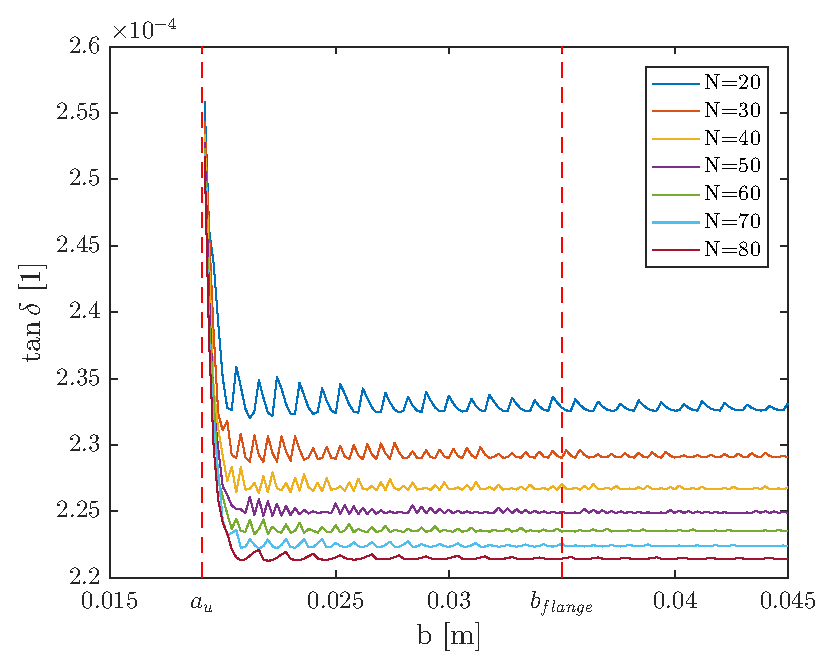
\includegraphics[scale=0.75]{b_conv_tand.eps}
\caption{Convergence plot of the loss tangent \tand{} against the radius of the sample region $b$ (flange diameter). The convergence is plotted for different numbers of modes $N=20,30,40,50,60,70,80$, where $N$ refers to the number of modes in the upper cavity for optimum mode ratios (i.e. for optimum relative convergence). The resonant frequency used for the plot was \SI{9.6619}{\giga\hertz}, the unloaded quality factor $Q_0$ of the resonance was \num{8754.3} and the thickness of the sample was \SI{1.509}{\milli\meter}. The upper cavity radius $a_u$ and the flange radius radius b\st{flange} are both marked with dashed vertical lines.}\label{fig:b_tand}
\end{figure}

\begin{figure}
\centering
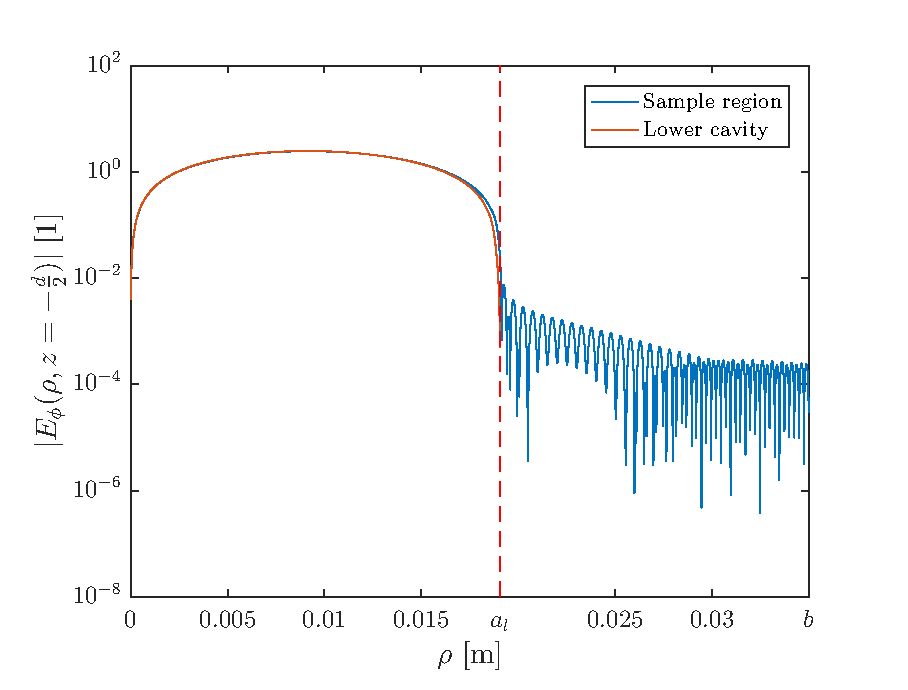
\includegraphics[scale=0.75]{E_phi_lower.eps}
\caption{M12 model - $\phi$ component of the normalised magnitude of the electric field for the sample region and for the lower cavity along their interface ($z=-\frac{d}{2}$). The radius of the lower cavity $a_l$ is marked with a dashed vertical line.}\label{fig:ephil}
\end{figure}
\begin{figure}
\centering
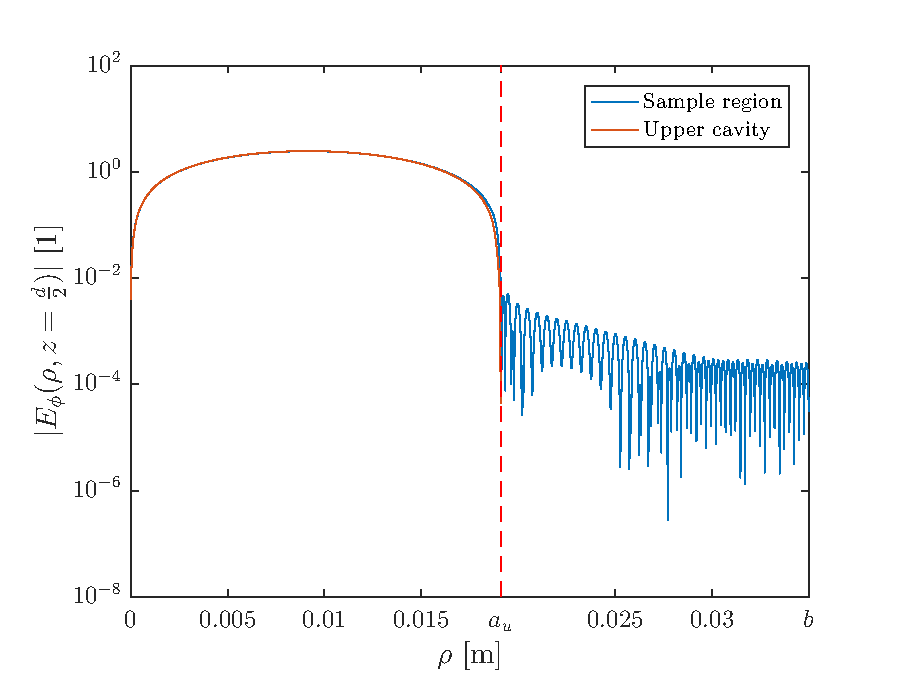
\includegraphics[scale=0.75]{E_phi_upper.eps}
\caption{M12 model - $\phi$ component of the normalised magnitude of the electric field for the sample region and for the upper cavity along their interface ($z=\frac{d}{2}$). The radius of the lower cavity $a_u$ is marked with a dashed vertical line.}\label{fig:ephiu}
\end{figure}

At the end of the last paragraph we mentioned that a sufficiently accurate approximation of the relative permittivity and the loss tangent of the resonator does not mean that the field in the resonator is approximated accurately. While our study of the relative convergence of the method clearly indicated that the functions of the relative permittivity and loss tangent are sufficiently smooth and converge to a true value with increasing numbers of modes, the underlying field configuration has not yet been examined. As the field in the resonator is a solution of the boundary-value problem of the split-cylinder resonator, we can check the field by looking at its boundary conditions. The boundary conditions that we need to check for this are not that of the perfectly conducting walls, which are naturally fulfilled by all modes in each region, but that of the interfaces. These are a figure of merit for how well the mode-matching method approximates the boundary value problem. As an example we examined the boundary conditions of a mode-matching calculation with $N=75$ modes that we made for the PTFE sample. Fig. \ref{fig:ephil} and \ref{fig:ephiu} illustrate that the tangential electric fields at both interfaces are very well matched. Over the entire aperture of each interface $0\leq\rho\leq a_{l,u}$ the electric fields on both sides are very similar and along the flange $a_{l,u}\leq \rho\leq b$ the electric field disappears as expected. As can be seen in Fig. \ref{fig:hrhol} and \ref{fig:hrhou} the magnetic field on the other hand is not very well matched at both interfaces. This is due to the conductor edges at $\rho=a_l$ and $\rho=a_u$ at the interface, which cause a singularity of the magnetic field (edge effect). A singularity causes a very rapid change in field strength, which cannot be approximated by the series expansions of the magnetic field. Similar to a Fourier series the spatial frequencies of the modes must be high enough to approximate a singularity. Another effect caused by the series expansion is the ripple of the approximations, which is also very similar to a Fourier series. Although the match of the magnetic field is relatively bad for this example, there is no need to worry. The magnetic field in this example is relatively weak at the boundary, so the singularity has a stronger influence on the field. Accordingly, the singularity also has less influence on the computed relative permittivity and loss tangent, as we have seen in the good convergence of the complex permittivity. The results for the calibration model were less suspicious: Fig. \ref{fig:ephical} and \ref{fig:hrhocal} show that both the tangential electric field $E_\phi$ and the tangential magnetic field $H_\rho$ were matched perfectly for the calbration, which was performed with a TE\st{011} mode at a resonant frequency of \SI{10.040}{\giga\hertz}.

\begin{figure}
\centering
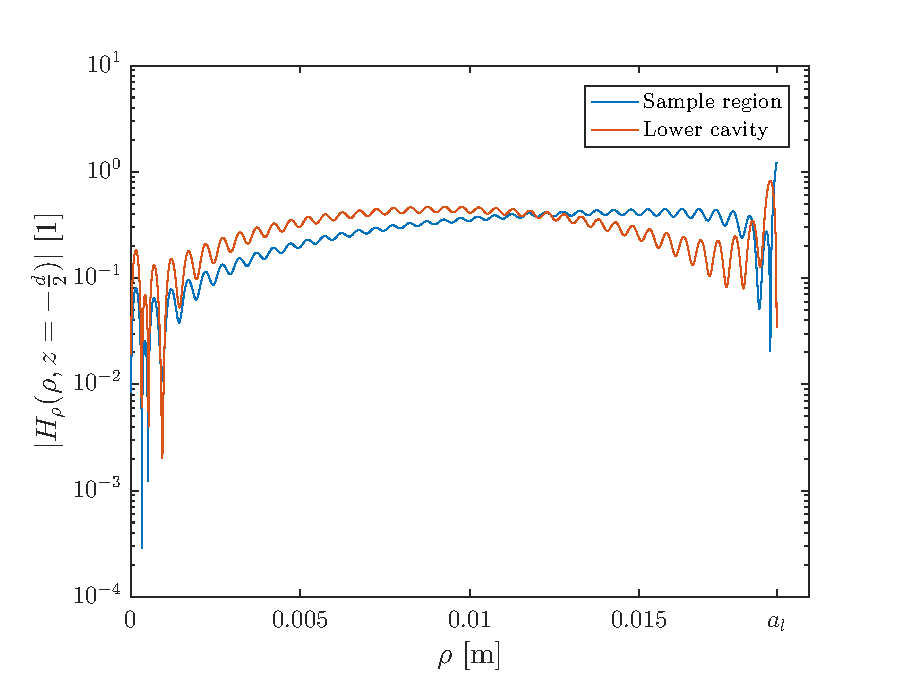
\includegraphics[scale=0.75]{H_rho_lower.eps}
\caption{M12 model - $\rho$ component of the normalised magnitude of the magnetic field for the sample region and for the lower cavity along their interface ($z=-\frac{d}{2}$).}\label{fig:hrhol}
\end{figure}
\begin{figure}
\centering
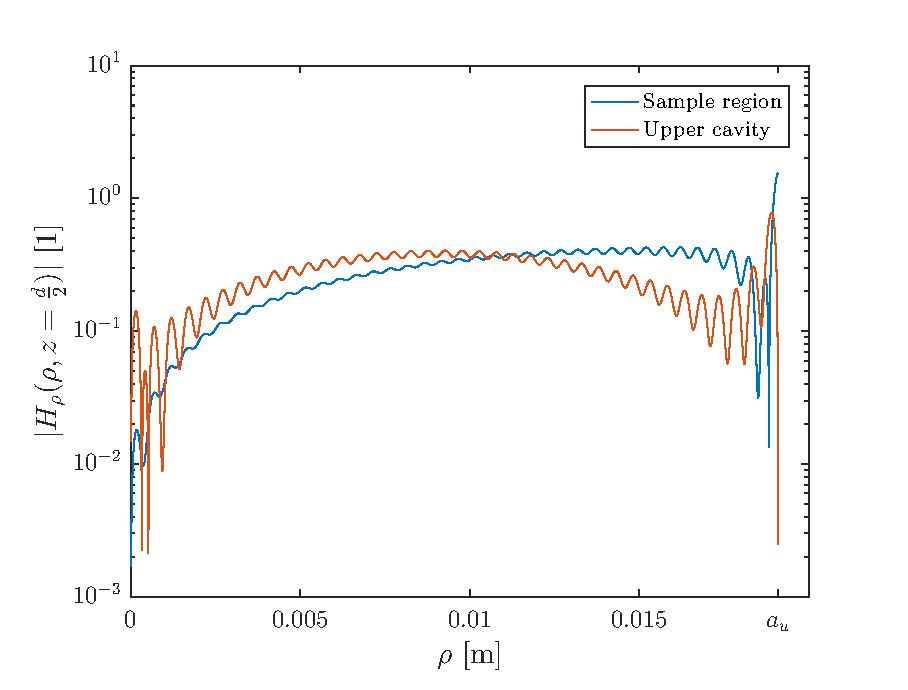
\includegraphics[scale=0.75]{H_rho_upper.eps}
\caption{M12 model - $\rho$ component of the normalised magnitude of the magnetic field for the sample region and for the upper cavity along their interface ($z=\frac{d}{2}$).}\label{fig:hrhou}
\end{figure}
\begin{figure}
\centering
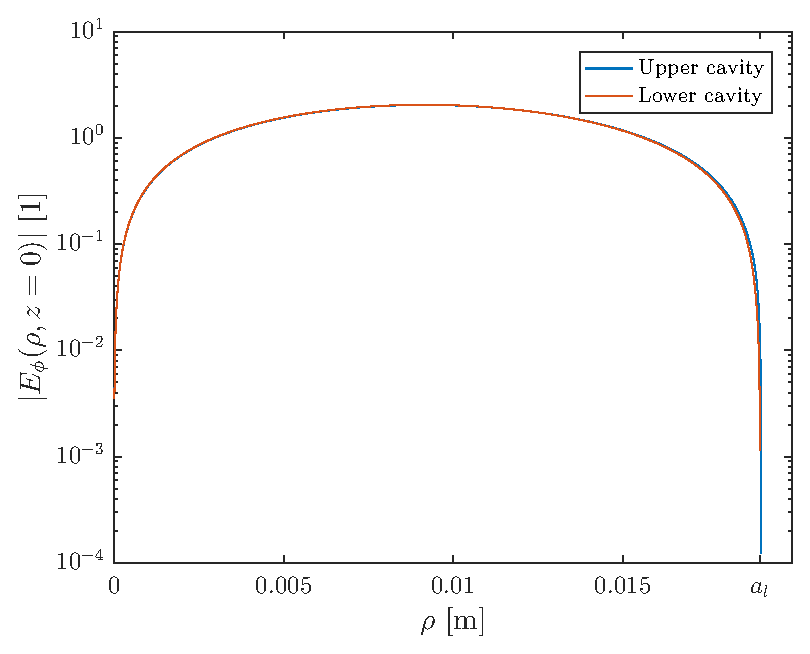
\includegraphics[scale=0.75]{E_phi_cal.eps}
\caption{Calibration model - $\phi$ component of the normalised magnitude of the electric field for the upper cavity and for the lower cavity along their interface ($z=0$).}\label{fig:ephical}
\end{figure}
\begin{figure}
\centering
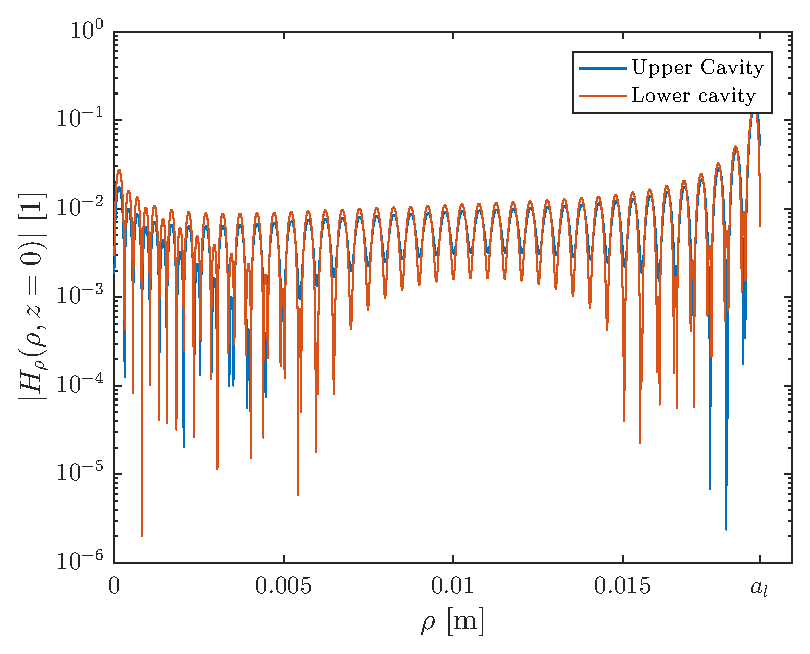
\includegraphics[scale=0.75]{H_rho_cal.eps}
\caption{Calibration model - $\rho$ component of the normalised magnitude of the magnetic field for the upper cavity and for the lower cavity along their interface ($z=0$).}\label{fig:hrhocal}
\end{figure}     % M12 model
\chapter{Measurement Results}\label{ch:results}
\section{Measurement Setup}
Fig. \ref{fig:setup} shows the measurement setup of a split cylinder resonator prototype that we developed and used for our measurements. In our setup the cylindrical cavities of the resonator were placed in a v-shaped groove of a hard wood base. The groove was clad with an aluminium sheet to avoid wear of the wooden base. Unlike other split cylinder resonator setups, our arrangement was self-aligning, which greatly simplified the setup. To provide enough room for large sheet samples we cut a slot into the base, in which large specimen may be inserted. A simple clamp mechanism was also added, which allowed us to firmly clamp the sample between the two cavities.

The cavities themselves were manufactured on a general purpose lathe from leaded brass (CuZnPb3). The blind holes of the cavities were first drilled, then the openings were enlarged using a boring bar. The face of the cavities, which are the flanges of the resonator, were also shaped in the same step to ensure proper alignment. The surface roughness of the cuts was note refined by any additional process like surface grinding or lapping. Generally speaking, a good surface finish guarantees high quality factors of the resonances, since a rough surface will have a higher surface impedance. High quality factors are essential for dielectric measurements with resonators, because resonances with a high quality factor have a narrow bandwidth and will therefore be less likely disturbed by neighbouring modes. In the light of this fact one might argue that lead brass with its relatively low bulk conductivity of \SI{15}{\mega\siemens\per\meter} is a bad choice as material for the cavities, since the conductivity is far lower than that of copper (\SI{58}{\mega\siemens\per\meter}) or silver (\SI{63}{\mega\siemens\per\meter}). It is widely noted that brass is still an excellent choice as material for cavities, because it is easily machinable and can be electroplated with better conductors to improve its conductivity. Still, we do not gain much from a better conductor on the cavity walls, since the quality factor is only proportional to the square root of the conductivity, $Q\propto\sqrt{\sigma}$. We measured a surface conductivity of around \SI{10}{\mega\siemens\per\meter} for our cavities, if we changed the material for the best conductor available, which is silver with a bulk conductivity of \SI{63}{\mega\siemens\per\meter}, the quality factor would increase less than two and a half fold.
\begin{equation*}
\frac{Q_\text{Silver}}{Q_\text{Brass,m}}\leq\sqrt{\frac{63}{10}}=2.45
\end{equation*}
Of course, this also means that the bandwidth of the resonance would decrease less than two and a half fold, which shows that the potential gain in accuracy is limited. If the amount of dielectric loss in a measurement is high, the gain will be even smaller. Finishing processes like diamond turning or grinding may still be beneficial for the performance of a cavity, since these processes typically have a higher manufacturing accuracy. Higher manufacturing accuracy also means lower uncertainty for the geometry of the apparatus, which in turn can increase the accuracy of dielectric measurements.

\begin{figure}
\centering
\begin{tikzpicture}
%\draw[step=0.25cm,gray,very thin] (-2,0) grid (13,7);
    \node[anchor=south west,inner sep=0] (image) at (0,0) {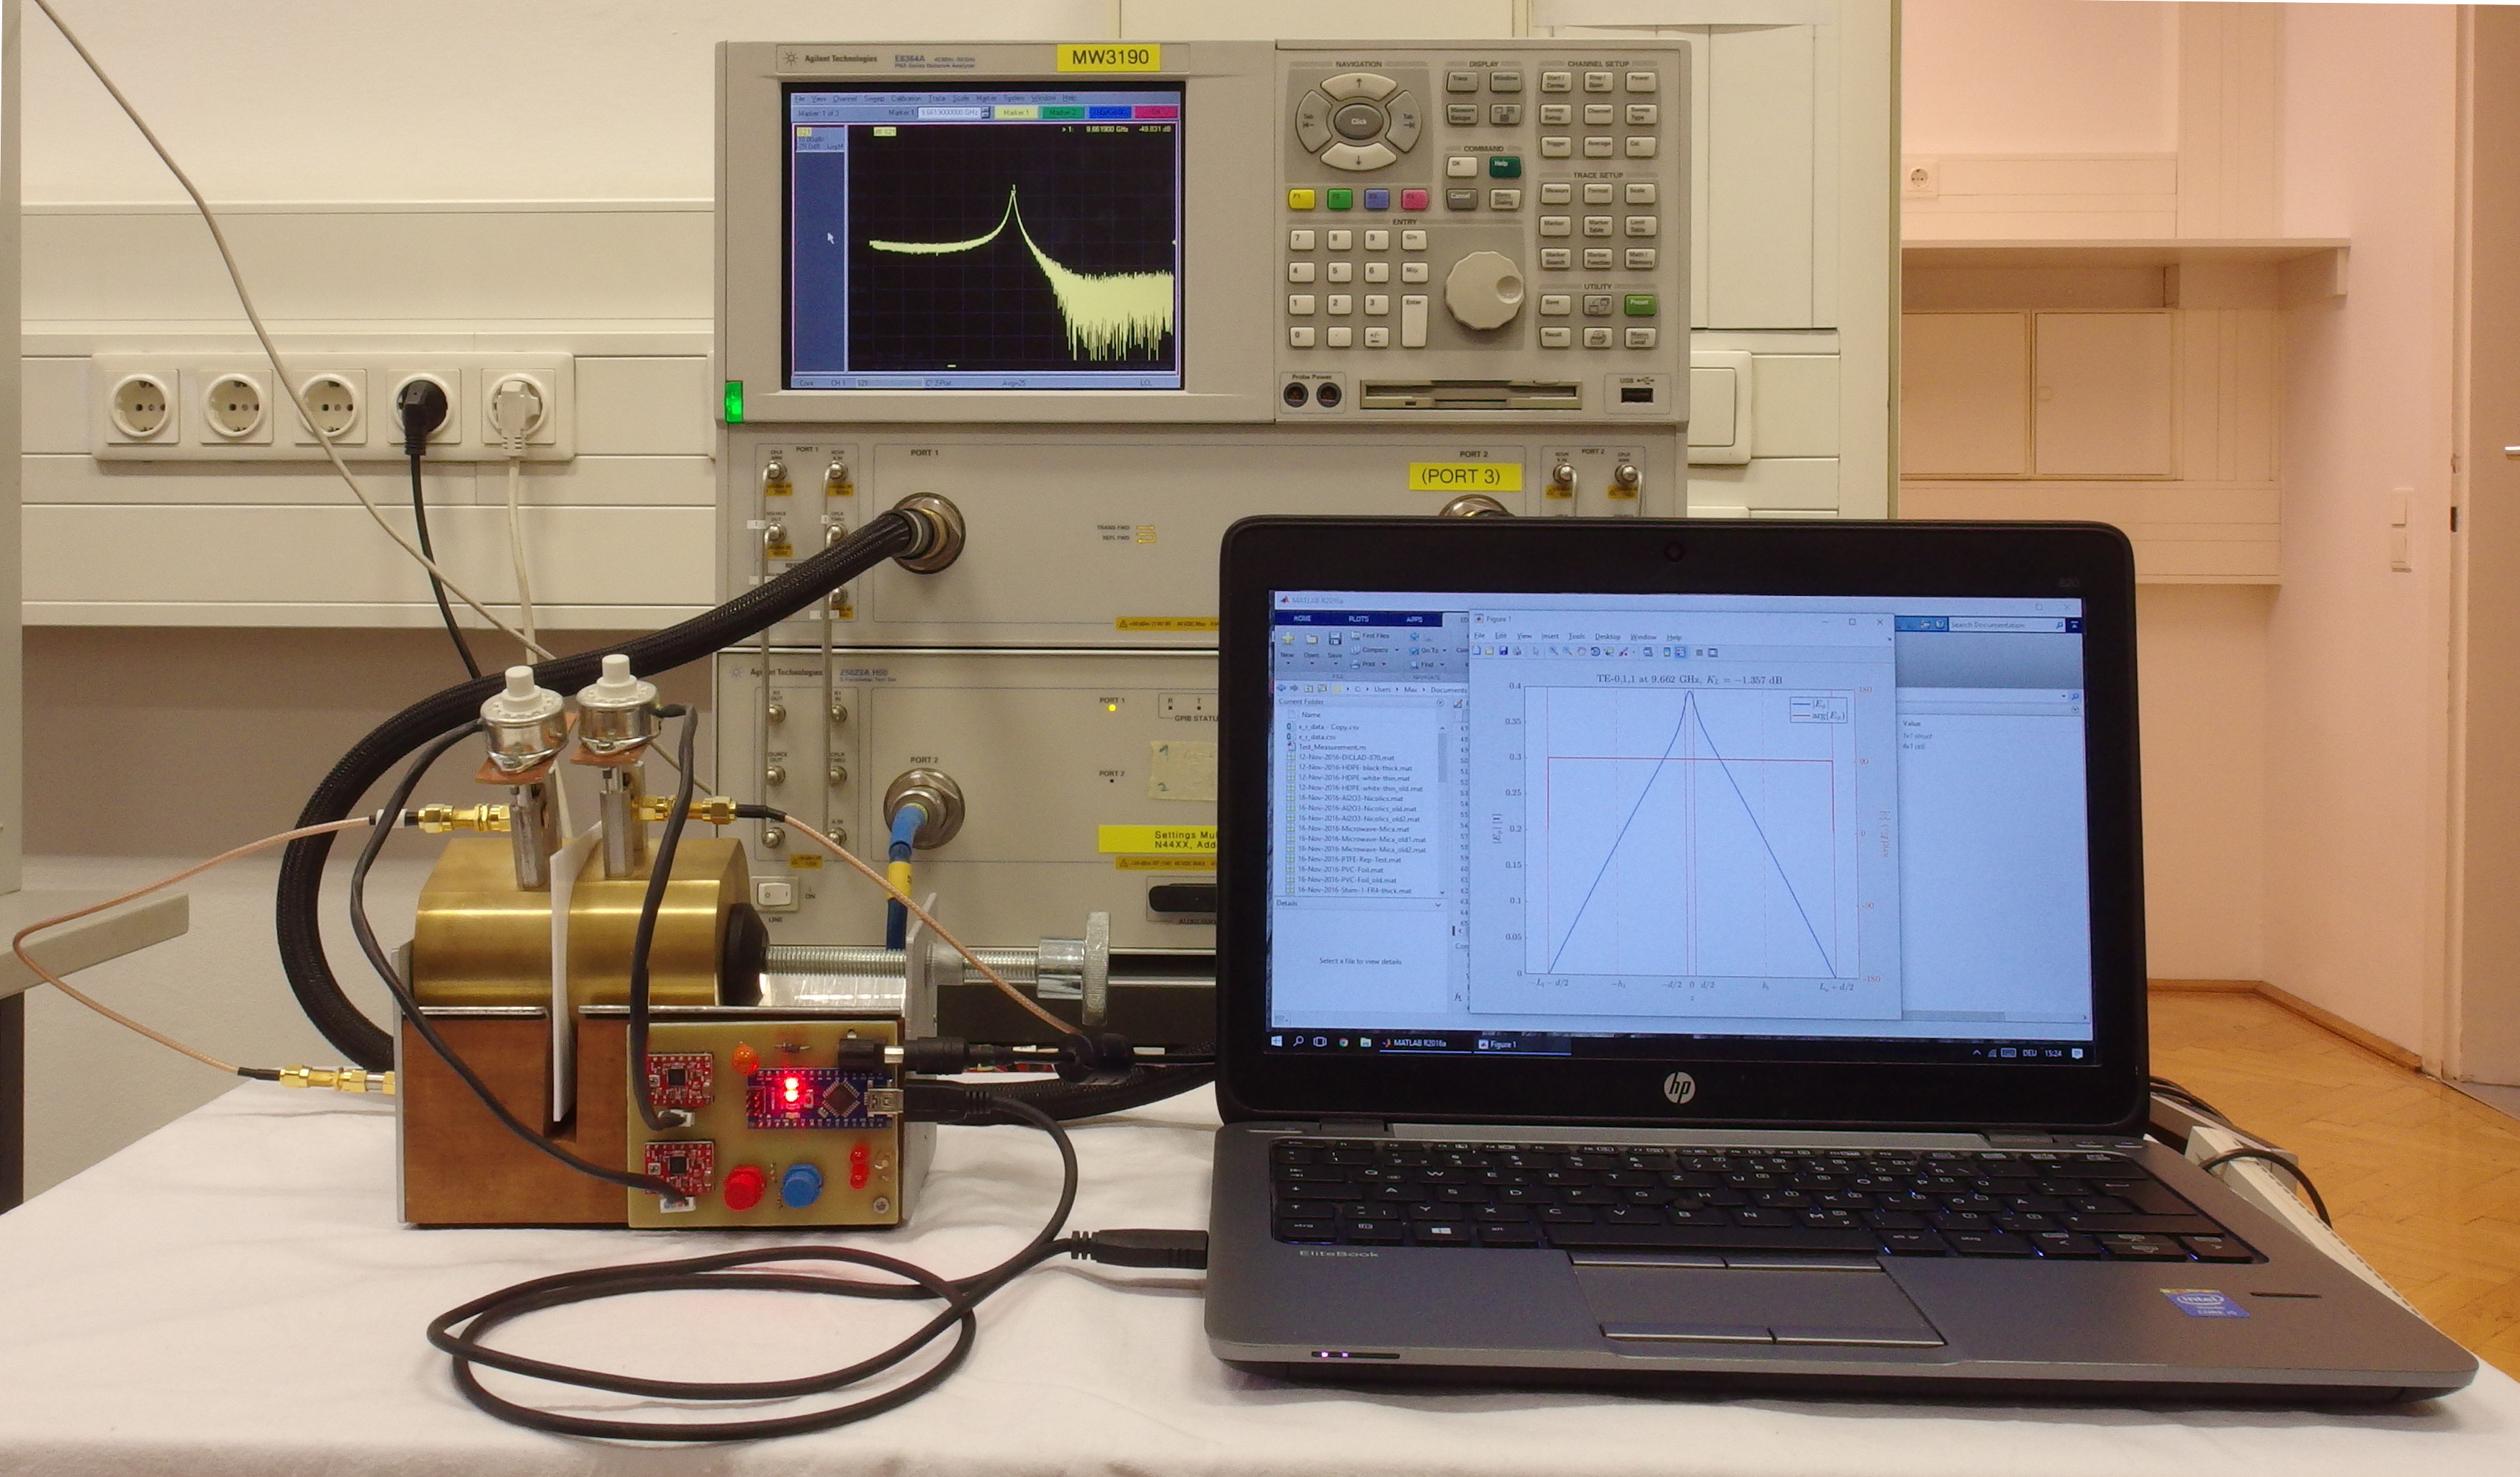
\includegraphics[height=6.45cm]{Measurement_setup_cropped.jpg}};
    
    \draw [-latex, thick, red] (-0.25,2.25) node[anchor=east, black,text width=2cm,align=right] {Resonator} to (1.8,2.25);
    \draw [-latex, thick, red] (-0.25,5.5) node[anchor=east, black,text width=2cm,align=right] {Coupling adjustment mechanisms} to (2.15,3.35);
    \draw [-latex, thick, red] (-0.25,5.5) to (2.65,3.625);    
    \draw [-latex, thick, red] (-0.25,0.75) node[anchor=east, black,text width=2cm,align=right] {PTFE sample} to (2.43,1.75);
    \draw [-latex, thick, red] (-0.25,3.75) node[anchor=east, black,text width=2cm,align=right] {Coaxial lines} to (0.8,2.65);
    \draw [-latex, thick, red] (-0.25,3.75) to (4,2.5);
    
    \draw [-latex, thick, red] (11.22,5.5) node[anchor=west, black,text width=2cm,align=left] {VNA} to (7.4,5);
    \draw [-latex, thick, red] (11.22,3.25) node[anchor=west, black,text width=2cm,align=left] {PC} to (9.4,3);    
    \draw [-latex, thick, red] (11.22,1) node[anchor=west, black,text width=2cm,align=left] {USB cable} to (4.25,0.5);

\end{tikzpicture}
\caption{Photograph of the measurement setup.}\label{fig:setup}
\end{figure}

The cavities were coupled to a vector network analyser by means of magnetic coupling loops, which were inserted into holes drilled into the cavities. The coupling loops were made from RG405 semi-rigid coaxial cable by soldering the inner conductor onto the outer conductor. To make the coupling adjustable we developed an electronic coupling adjustment mechanism. This mechanism works as such that the coupling loops are mounted on the shanks of two linear stepper motors. When the stepper motors extend the shanks, the coupling loops are lowered into the cavities and the coupling increases. Conversely, when the shanks are pulled up by the stepper motors, the loops are moved out of the cavity and the coupling decreases. The two stepper motors were driven by an electronic circuit, which could be remote controlled from a PC. The interface with a PC allowed the measurement software to adjust the coupling of the resonator, which was especially useful for broadband measurements. In a cavity the coupling coefficients vary from mode to mode, so the coupling needs to be adjusted for every mode to keep the coupling coefficient at the desired level. The electronic adjustment mechanism simplifies the measurement procedure and speeds up the measurement compared to a manual adjustment mechanism. Additionally, the stepper motors we used had a linear travel per step of only \SI{1}{thou} (\SI{25,4}{\micro\meter}), which also allowed to us to adjust the coupling more precisely. Besides allowing us to fine-tune the coupling, the stepper motors also made it possible to adjust the coupling symmetrically and keep the symmetry while adjusting the coupling. As we have discussed previously, symmetric coupling allows us to determine the coupling coefficient from the maximum of the transmission coefficient. The coupling coefficient of a very under-coupled resonator is almost negligible, but symmetric coupling may be used to improve the accuracy of our quality factor measurements.

The measurement results were computed with a measurement software written in the MATLAB scripting language. It was designed by us as a software suite for calibrations and measurements with a split cylinder resonator. The software was run by a PC next to the vector network analyser (VNA), which was connected to the VNA through an ethernet connection and to the coupling adjustment circuit through a USB connection. A wide range of different features of the software were used in our measurements. The software set up the transmission coefficient measurements on the VNA, fetched the measurement data and saved it on the PC for later use. It also determined the resonances of the frequency response of the transmission coefficient and adjusted the coupling appropriately through the electronic adjustment mechanism. From the measured resonance curves it determined the quality factor and the resonant frequency of the resonance. The software supported a wide range of different quality factor measurement techniques like the 3dB method, the Coakley method and a circle-fit. The measurement results of the quality factor measurements were then used by the software to compute the relative permittivity and the loss tangent for the TE\st{011} modes as well as higher modes. Or, if the software was in calibration mode, it was used to calculate the calibration radius $a_l$ and the conductivity $\sigma$. If the calibration data was used in a measurement, the software allowed the operator to use different calibrations for different modes (broadband calibration). The software supported both the Janezic model and our very own M12 model. Finally, if the resonant frequency of the TE\st{011} mode or any other higher TE\st{0np} mode was unknown, the software had a feature to estimate the permittivity from the fundamental mode. This estimate could then be used to estimate the resonant frequency of the mode in question.
\section{Measurement Flow}
\begin{figure}
\centering
% Define block styles
\tikzstyle{block} = [rectangle, draw, fill=blue!20, 
    text width=6.3em, text centered, rounded corners, minimum height=3.5em]
\tikzstyle{line} = [draw, -latex',font=\fontsize{9}{9}]
    
\begin{tikzpicture}
    % Place nodes
    \node [block] (empty_res) {Empty resonator characterisation};
    \node [block, below of=empty_res, node distance=2cm] (cal) {Calibration};        
    \node [block, right of=cal, node distance=3.7cm] (esti) {TE\st{0np} resonant frequency estimation};
    \node [block, below of=esti,node distance=2cm] (meas) {Transmission coefficient measurement};
    \node [block, right of=esti, node distance=3.5cm] (eresti) {Relative permittivity estimation};
    \node [block, left of=cal, node distance=4.2cm] (length) {Resonator dimensions measurement};
    \node [block, below of=meas, node distance=2cm] (calc) {$\varepsilon_r$ and $\tan\delta$ calculation};
    \node [block, above of=esti, node distance=2cm] (thickness) {Sample thickness measurement};
    \node [block, below of=calc, node distance=2cm] (uncert) {Uncertainty estimation};
    \node [coordinate, below of=uncert, node distance=1.2cm] (bert) {Uncertainty estimation};
    % Draw edges
    \draw[dashed] (1.85,0.5) -- (1.85,-9.5);
    \path [line] (empty_res) -- node[anchor=east] {$f_\text{r,empty}$, $Q_\text{0,empty}$} (cal);
    \path [line] (cal) -- node[anchor=south] {$a_l, \sigma$} (esti);
    \path [line] (esti) -- node[anchor=west] {$f_{r,\text{est}}$} (meas);
    \path [line] (eresti) -- node[anchor=south] {$\epsilon_{r,\text{est}}$} (esti);
    \path [line] (meas) -- node[anchor=west] {$f_r, Q_0$} (calc);
    \path [line] (calc) -- node[anchor=west] {$\epsilon_r,\tan\delta$} (uncert);
    \path [line] (thickness) -- node[anchor=west] {$d$} (esti);
    \path [line] (length) -- node[anchor=south] {$L_l$, $L_u$, $a_u$} (cal);
    \path [line] (uncert) -- (bert) node[anchor=north] {$u(\varepsilon_r),u(\tan\delta)$};
\end{tikzpicture}
\caption{Flow diagram of a measurement with the M12 model.}\label{fig:flow}
\end{figure}

The flow diagram shown in Fig. \ref{fig:flow} illustrates the individual steps of a measurement with the M12 model. Although we have already discussed many aspects of the measurement like the theory of the model, the calibration of the resonator or quality factor measurements of resonance curves, it is  still worthwhile to take a closer look at the measurement process and to explain how the different steps of a measurement interact. When we take a look at the measurement shown in the flow diagram, the first thing that strikes us is the dashed line in the middle of the diagram.  This line divides the measurement process into two procedures, the calibration procedure on the left hand side and the measurement procedure on the right hand side. The blocks shown in the diagram are the step of these two procedures and the lines connecting the blocks are the variables that are determined in the step they originate from. The line crossing the dashed line separating the two procedures carries along the calibration variables from the calibration to the measurement procedure and connects the two procedures.

In the calibration procedure one of the first steps is the measurement of the resonator dimensions, which determines the lengths of the cavities $L_u$ and $L_l$, and the radius of the upper cavity $a_u$. Both should be measured accurately with a calliper or a micrometer. In the next step, the empty resonator characterisation, the cavities are pressed together to form a cylindrical cavity, and the resonant frequencies and quality factors of the resonant modes of the cavity are measured. These and the resonator dimension are then handed over to the last step in the calibration, which calculates the radius of the lower cavity $a_l$ and conductivity $\sigma$ for each of the calibration modes.

This step ends the calibration and delivers the calibration parameters to the measurement procedure. The first step in the measurement procedure is the estimation of the resonant frequencies of the TE\st{0np} modes. As this step uses the M12 model to estimate the resonant frequencies, all dimensions of the resonator are required. Out of this reason the thickness of the sample needs to be measured, for example with a micrometer. Apart from the sample thickness measurement, which gives the thickness $d$ of the specimen, estimating the resonant frequencies of the modes also requires an estimate for the relative permittivity of the specimen $\epsilon_{r,est}$. This relative permittivity of the specimen can be estimated, for example, from a value in a data sheet or from a measurement of the fundamental TE\st{111} mode of the split cylinder resonator. With these two parameters the resonant frequencies are estimated and passed on to the next step, the transmission coefficient measurement. In this step the sample is inserted into the resonator and the transmission coefficient is measured around the estimated resonant frequencies. If there is no overlap with other modes, this measurement yields the resonance curves of the TE\st{0np} modes. These curves are then used to calculate the resonant frequencies $f_r$ and quality factors $Q_0$ of the modes. Finally, this brings to the most interesting step of the measurement, the calculation of the relative permittivity and loss tangent of the sample. In this step the relative permittivity and the loss tangent of the sample are calculated from the resonator dimensions, the resonant frequencies and the quality factors of the modes using the M12 model. This calculation yields the results of the measurement. Lastly, the uncertainty of the measurement can be estimated, if multiple measurements of the specimen and the calibration are performed. 
\section{Uncertainty Budget of the M12 Matrix Model}
%%%%%%%%%%%%%%%%%%%%%%%%%%%%%% UNCERTAINTY BUDGET COMMAND %%%%%%%%%%%%%%%%%%%%%%%%%%%%%%%%%%%%%
\newcolumntype{C}[1]{>{\centering\let\newline\\\arraybackslash\hspace{0pt}}m{#1}}
\newcommand{\uncertbl}[2]{
\pgfplotstabletypeset[sci zerofill,precision=2,font=\scriptsize,
					  col sep=tab,
                      every head row/.style={before row=\hline\rule{0pt}{2.6ex}
										     #1 & \multicolumn{7}{c|}{ }\\\hline\rowcolor{gray!20}\rule{0pt}{2.6ex},after row=\hline\rule{0pt}{2.6ex}},
					  columns={symb,sourceu,value,unit,pdf,div,coeff,ui},
                      every last row/.style={after row=\hline},
                      columns/symb/.style={column type=|C{0.06\textwidth},column name=Symb.,string type},
                      columns/sourceu/.style={column type=|C{0.18\textwidth},column name={Source of uncertainty},string type},	
					  columns/value/.style={column type=|C{0.09\textwidth},column name={Value $\pm$}},
					  columns/unit/.style={column type=C{0.04\textwidth},column name={Unit},string type},
					  columns/pdf/.style={column type=|C{0.16\textwidth},column name={Probability dist.},string type},		
         		      columns/div/.style={column type=|C{0.03\textwidth},column name={Div.},string type},
					  columns/coeff/.style={column type=|C{0.09\textwidth},column name={$c_i$}},
					  columns/ui/.style={column type=|C{0.09\textwidth}|,column name={$u_i$}},
                      %columns/vi/.style={column type=|C{0.05\textwidth}|,column name={$\nu_i$},string type},
                      empty cells with={ },
						]#2}
%%%%%%%%%%%%%%%%%%%%%%%%%%%%%%%%%%%%%%%%%%%%%%%%%%%%%%%%%%%%%%%%%%%%%%%%%%%%%%%%%%%%%%%%%%%%%%%%%
This section deals with the uncertainty of a measurement with the M12 model and compares it to the uncertainty of measurements with the Janezic model. In the title of this thesis we emphasised that this model is an improved model for complex permittivity measurements with a split-cylinder resonator. Our model is in principle an expansion of the Janezic model and also uses mode-matching to solve the field problem. Still, our model solves the field problem for a cavity with unequal half-cavities, which eliminates the systematic error of the symmetric model. As we will see later in this section, this can reduce the uncertainty of a relative permittivity measurement by more than 70\% and, hardly noticeable, that of loss tangent measurements by around 5\%. 

To illustrate the improvements in accuracy we have calculated the uncertainty budget of a measurement. For this measurement we measured the same PTFE sample that we have used for most of our previous examples. The measurements were performed with \te{} modes at a constant ambient temperature of around \SI{22}{\celsius}. The calculation of the uncertainty budget included Type A and Type B uncertainties, where Type A refers to uncertainties evaluated by a statistical analysis of a series of observations and Type B roughly refers to systematic uncertainties. An in-detail explanation of these two kinds of uncertainties can be found in a guide published by UKAS \cite{UKAS} and in the GUM \cite{GUM}. The Type A uncertainties were evaluated in a repeatability evaluation (Sec. \ref{sec:rep}) of the calibration and of the complex permittivity measurement. With respect to the statistical analysis of the measurement values, we decided to report all expanded uncertainties for a coverage probability of close to 95\%, which required a coverage factor of around 2 for a Gaussian distribution. Unlike many other researchers, our evaluations were performed under a worst-case assumption, and hence we used uniform distributions for all inputs with a unknown probability distribution. Since the probability distribution and the coverage of random variables with input variables that have a uniform distribution is not Gaussian, we used a Monte-Carlo simulation (NIST uncertainty machine) to compute the probability distributions and coverage factors for all variables.

The quality factor and resonant frequency of the measurement modes were obtained from transmission coefficient measurements with a Keysight PNA E8364A vector network analyser. The VNA was calibrated at a right-angle SMA connector that connected the coupling loops to the coaxial lines of the VNA. The calibration was performed with a Keysight N4433A electronic calibration module, which also limited the frequency range of our measurements to less than \SI{20}{\giga\hertz}. To ensure good linear performance and high dynamic range the output power of the VNA was set to \SI{0}{dBm}, which improved the measurement accuracy for small transmission coefficients in the \SIrange{-70}{-50}{\decibel} range. Each measurement was an average over 25 measurement sweeps, which were measured with the default IF bandwidth of \SI{35}{\kilo\hertz}. For this configuration we estimated the accuracy of the transmission coefficient measurement using the Keysight VNA uncertainty calculator. The calculator estimated an accuracy of less than \SI{0.93}{\decibel} for the magnitude and an accuracy of less than \SI{6.5}{\degree} for the phase in the \SIrange{-70}{-50}{\decibel} range. Using these accurate transmission coefficient measurements we were able to measure the quality factor and the resonant frequency very accurately. We evaluated the uncertainty of the quality factor measurements using the findings of Petersan and Anlage \cite{petersan}, see Sec. \ref{sec:rescurve}. The quality factors and resonant frequencies were measured using a circle-fit of the measured resonance curves. All resonance curves of the calibration and of the permittivity measurements had SNRs (for a definition of this SNR, please refer to \cite{petersan}) exceeding 60. Petersan and Anlage found that the relative accuracy of a circle-fit, which is more or less identical to the phase vs. frequency fit discussed in their article, for such high SNRs and a quality factor of around \num{e3} was less than \num{7.88e-8} for the resonant frequency and less than \num{1.3e-4} for the quality factor. Although the relative precision of the quality factor was lower than the accuracy of the method, we evaluated the uncertainty of the quality factor measurements using only the relative accuracy. This was acceptable as the quality factor measurements were found to have a negligible influence on our calibration parameters and on our permittivity measurements. For lower SNRs a more accurate analysis should be performed. 

\subsection{Uncertainty of Dimensional Measurements}
\begin{table}[ht]
\centering
%%% UNCERTAINTY OF L						
\pgfplotstableread[col sep=tab]{
symb	sourceu	value	unit	pdf	div	coeff	ui	vi
u\st{r}	Flatness	3.70E-05	m	Uniform	$\sqrt{3}$	1	2.14E-05	∞
u\st{m}	Calliper	2.11E-05	m	Uniform	$\sqrt{3}$	1	1.22E-05	∞
u(L)	Combined uncertainty		m	Convolved			2.46E-05	∞
U	Expanded uncertainty		m	Convolved (k=1.9)			4.67E-05	∞
}\uncertl
\uncertbl{$L$}{\uncertl}
\caption{Uncertainty budget of $L$ of the Janezic model.}\label{u:L}
\end{table}

Starting point for any measurement with a split-cylinder resonator are dimensional measurements of the resonator. In the \textbf{Janezic model} the only dimension that had to be measured is the length $L$ of the cavities. The cavity length $L$ was measured with a digital calliper along the circumference of the bore. Each cavity was measured 20 times. The dimensional uncertainty of $L$ was evaluated using a uniform distribution, which used the sample mean of these measurements as mean $\mu_L$ and the largest difference $u_r=\Delta_L$ of a measurement value from the sample mean as half-width of the uniform distribution:
\begin{equation}
f_L(L)=\begin{cases}\frac{1}{2\Delta_L}, & \mu_L-\Delta_L\leq L\leq \mu_L+\Delta_L\\
					0, & \text{elsewhere} \\
	    \end{cases}
\end{equation}
We used the uniform distribution in line with our worst-case assumption for the evaluation of uncertainty. The expanded uncertainty of the depth measurements at a coverage probability of 95\% was $\text{MPE}_E+\text{MPE}_S=\SI{40}{\micro\meter}$ in accordance with DIN862. Similar to the dimensional uncertainty, the uncertainty of depth measurements was evaluated using a uniform distribution with $u_m=\frac{1}{0.95}(\text{MPE}_E+\text{MPE}_S)=\SI{42.1}{\micro\meter}$. The uncertainty budget of $L$ is shown in Table \ref{u:L}.

\begin{table}[ht]
\centering

%%% UNCERTAINTY OF L_U						
\pgfplotstableread[col sep=tab]{
symb	sourceu	value	unit	pdf	div	coeff	ui	vi
u\st{r}	Flatness	9.00E-06	m	Uniform	$\sqrt{3}$	1	5.20E-06	∞
u\st{m}	Calliper	2.11E-05	m	Uniform	$\sqrt{3}$	1	1.22E-05	∞
u($L_u$)	Combined uncertainty		m	Convolved			1.32E-05	∞
U	Expanded uncertainty		m	Convolved (k=1.8)			2.38E-05	∞
}\uncertlu
\uncertbl{$L_u$}{\uncertlu}

\vspace{7px}

%%% UNCERTAINTY OF L_L						
\pgfplotstableread[col sep=tab]{
symb	sourceu	value	unit	pdf	div	coeff	ui	vi
u\st{r}	Flatness	2.30E-05	m	Uniform	$\sqrt{3}$	1	1.33E-05	∞
u\st{m}	Calliper	2.11E-05	m	Uniform	$\sqrt{3}$	1	1.22E-05	∞
u(L\st{l})	Combined uncertainty		m	Convolved			1.80E-05	∞
U	Expanded uncertainty		m	Convolved (k=1.9)			3.42E-05	∞
}\uncertll
\uncertbl{$L_l$}{\uncertll}

\vspace{7px}

%%% UNCERTAINTY OF A_U
\pgfplotstableread[col sep=tab]{
symb	sourceu	value	unit	pdf	div	coeff	ui	vi
{u\st{taper}}	Taper	4.62E-06	m	Uniform	$\sqrt{3}$	1	2.67E-06	∞
{u\st{m}}	Inside Micrometer	2.11E-06	m	Uniform	$\sqrt{3}$	1	1.22E-06	∞
u($a_u$)	Combined uncertainty		m	Convolved			2.93E-06	∞
U	Expanded uncertainty		m	Convolved (k=1.8)			5.28E-06	∞
}\uncertau
\uncertbl{$a_u$}{\uncertau}
\caption{Uncertainty budget of $a_u$, $L_u$ and $L_l$ of the M12 model.}\label{u:Ll}
\end{table}

For the \textbf{M12 model} the situation was a bit more complicated, because the radius of the upper cavity $a_u$, the length of the lower cavity $L_l$ and the length of the upper cavity $L_u$ had to be measured. The radius $a_u$ was measured ten times at three different depths of the bore using a bore gauge. As probability distribution a uniform distribution was chosen for the radius, which used the sample mean as mean value and the largest deviation of a measurement value from the mean as half-width of the distribution. The gauge had an expand uncertainty for the diameter of \SI{4}{\micro\meter} in accordance with DIN863-4. The lengths of the cavities were measured in the same way as for the Janezic model, only the uncertainty was evaluated individually for each cavity. The uncertainty budgets of $a_u$, $L_l$ and $L_u$ are shown in Table \ref{u:Ll}.

\begin{table}[ht]
\centering
%%% UNCERTAINTY OF D
\pgfplotstableread[col sep=tab]{
symb	sourceu	value	unit	pdf	div	coeff	ui	vi
{u\st{flat}}	Flatness	3.85E-06	m	Uniform	$\sqrt{3}$	1	2.22E-06	∞
{u\st{m}}	Micrometer	4.21E-06	m	Uniform	$\sqrt{3}$	1	2.43E-06	∞
u(d)	Combined uncertainty		m	Convolved			3.29E-06	∞
U	Expanded uncertainty		m	Convolved (k=1.9)			6.26E-06	∞
}\uncertd
\uncertbl{$d$}{\uncertd}
\caption{Uncertainty budget of $d$.}\label{u:d}
\end{table}

The \textbf{thickness $\mathbf{d}$} of the Janezic model and of the M12 model were identical, likewise the uncertainties were evaluated in the same way. The thickness of the PTFE sample was measured twenty times - each time at a different location on the sample - using an outside micrometer. We used the sample mean as the mean of $d$, and the largest deviation of a measurement value $u_\text{flat}=\Delta_d$ from the mean as the error due to thickness variations of the sample. In line with our worst-case assumption the error had a uniform distribution. The measurements were performed with a digital outside micrometer, which was put in a small vice to avoid measurement errors due to thermal expansion of the micrometer frame. The micrometer had an expanded uncertainty (MPE) of \SI{4}{\micro\meter} according to DIN863-1. The measurement error of the micrometer was modelled with a uniform distribution, which had a half-width of $u_m=\frac{1}{0.95}\text{MPE}=\SI{4.21}{\micro\meter}$. The uncertainty budget of $d$ is shown in Table \ref{u:d} and all dimensions and the thickness of the sample are listed in Table \ref{u:dim}. 

\begin{table}[ht]
\centering
\scriptsize
\newcolumntype{P}{>{\centering\arraybackslash}p{0.125\textwidth}}
\begin{tabular}{|P|P|P|P|P|P|}
\hline \rule{0pt}{2.6ex}
 & $\mathbf{L}$ & $\mathbf{L_u}$ & $\mathbf{L_l}$ & $\mathbf{a_u}$ & $\mathbf{d}$ \\ 
\hline \rule{0pt}{2.6ex}
Mean $\mu$ & \SI{25.023}{\milli\meter} & \SI{25.009}{\milli\meter} & \SI{25.037}{\milli\meter} & \SI{19.09}{\milli\meter} & \SI{1.5092}{\milli\meter} \\ 
\hline \rule{0pt}{2.6ex}
Half-width $\pm\Delta$ & \SI{37}{\micro\meter} & \SI{9}{\micro\meter} & \SI{23}{\micro\meter} & \SI{4.62}{\micro\meter}  & \SI{3.85}{\micro\meter}  \\ 
\hline \rule{0pt}{2.6ex}
Measurement & $20\times$ along perimeter of each cavity & 20x along perimeter & 20x along perimeter & 10x at three depth levels & 20x at various locations on sample \\ 
\hline \rule{0pt}{2.6ex}
Instrument & Calliper & Calliper & Calliper & Bore gauge & Outside micrometer \\ 
\hline
\end{tabular} 
\caption{Dimensions of the split-cylinder prototype and thickness of the sample.}\label{u:dim}
\end{table}

\subsection{Uncertainty of Permittivity Measurements}

\begin{table}
\centering
%%% UNCERTAINTY OF A CAL						
\pgfplotstableread[col sep=tab]{
symb	sourceu	value	unit	pdf	div	coeff	ui
f\st{r,cal}	Resonant frequency	7.91E+02	Hz	Normal	1	2.09E-12	1.65E-09
L	Cavity length	6.15E-05	m	Convolved (k=1.9)	1.9	7.44E-02	2.41E-06
{$\Delta$}	Difference from dimensional measurement	3.27E-05	m	Convolved (k=1.6)	1.6	1	2.04E-05
a\st{r}	Repeatability	8.49E-07	m	Normal	1	1	8.49E-07
u(a)	Combined standard uncertainty			Quasi-Normal			2.06E-05
U	Expanded uncertainty			Quasi-Normal (k=2)			4.03E-05
}\uncertja
\uncertbl{$a$}{\uncertja}

\vspace{7px}

%%% UNCERTAINTY OF SIGMA CAL						
\pgfplotstableread[col sep=tab]{
symb	sourceu	value	unit	pdf	div	coeff	ui
f\st{r,cal}	Resonant frequency	7.91E+02	Hz	Normal	1	1.00E-03	7.92E-01
Q\st{cal}	Quality factor	1.60	-	Normal	1	1.63E+03	2.61E+03
a	Cavity radius	4.03E-05	m	Quasi-Normal (k=2)	2	6.23E+07	1.26E+03
L	Cavity length	6.15E-05	m	Convolved (k=1.9)	1.9	4.75E+07	1.54E+03
σ\st{r}	Repeatability	2.23E+05	S/m	Normal	1	1	2.23E+05
u(σ)	Combined standard uncertainty			Quasi-Normal			2.23E+05
U	Expanded uncertainty			Quasi-Normal (k=2)			4.38E+05
}\uncertjsigma
\uncertbl{σ}{\uncertjsigma}
\caption{Uncertainty budget of $a$ and $\sigma$ of the Janezic calibration.}\label{u:cal_j}
\end{table}

Using the uncertainty budget of the dimensional measurements and the findings of Petersan and Anlage \cite{petersan}, we calculated the uncertainty budget of the calibration parameters and of the measurement results for the Janezic model and for the M12 model. In the uncertainty calculation all input variables were assumed to be independent random variables. To simplify the calculations correlations between the calibration parameters and the resonator dimensions were ignored. Computations including the correlations showed that these changed the results very little. Apart from that, the upper limit on the uncertainty guaranteed an uncertainty of less than the sum of all uncertainties, as stated by Taylor \cite[Sec. 9.2]{taylor}. 

We started the calculations by first determining the sensitivity coefficients $c_i$ of each model. These coefficients were computed with our measurement software and $N=75$ modes were included in each of the calculations. The coefficients for the uncertainty budget of the calibration were determined for a resonant frequency of $f_r=\SI{10.040}{\giga\hertz}$ and a quality factor of $Q=\num{12299}$. And, the coefficients for the uncertainty budget of the measurement were computed for a resonant frequency of $f_r=\SI{9.6619}{\giga\hertz}$, a quality factor of $Q=\num{8882}$, a thickness of the sample of $d=\SI{1.509}{\milli\meter}$ and a sample radius of $b=\SI{35}{\milli\meter}$. 

Secondly, we performed calibration measurements of the empty resonator and permittivity measurements of the PTFE sample 20 times to study the repeatability of each measurement. In these measurements, we rotated the cavities after each measurement, so that the orientation of the two half-cavities changed from measurement to measurement. This was done to account for the random error caused by the misalignment of the cavities in the mount. Before we conducted this repeatability evaluation, we first cleaned the resonator with soap to remove any dirt left by machining, then we cleaned resonator and sample with Isopropyl alcohol. After the cleaning we dried both of them thoroughly. 

\begin{table}
\centering
%%% UNCERTAINTY OF A_L CAL					
\pgfplotstableread[col sep=tab]{
symb	sourceu	value	unit	pdf	div	coeff	ui
f\st{r,cal}	Resonant frequency	7.91E+02	Hz	Normal	1	4.16E-12	3.29E-09
a\st{u}	Upper cavity radius	5.28E-06	m	Convolved (k=1.8)	1.8	9.95E-01	2.92E-06
L\st{u}	Upper cavity length	4.47E-05	m	Convolved (k=1.8)	1.8	7.31E-02	1.82E-06
L\st{l}	Lower cavity length	5.26E-05	m	Convolved (k=1.9)	1.9	7.57E-02	2.10E-06
{$\Delta$}	Difference from dim. measurement	1.44E-05	m	Convolved (k=1.7)	1.7	1	8.45E-06
a\st{l,r}	Repeatability	1.72E-06	m	Normal	1	1	1.72E-06
u(a\st{l})	Combined standard uncertainty			Quasi-Normal			9.51862E-06
U	Expanded uncertainty			Quasi-Normal (k=1.9)			1.80854E-05
}\uncertmal
\uncertbl{$a_l$}{\uncertmal}

\vspace{7px}

%%% UNCERTAINTY OF SIGMA CAL					
\pgfplotstableread[col sep=tab]{
symb	sourceu	value	unit	pdf	div	coeff	ui
f\st{r, cal}	Resonant frequency	7.91E+02	Hz	Normal	1	5.01E-03	3.96E+00
Q\st{cal}	Quality factor	1.60E+00	-	Normal	1	1.63E+03	2.61E+03
a\st{u}	Upper cavity radius	5.28E-06	m	Convolved (k=1.8)	1.8	4.98E+08	1.46E+03
a\st{l}	Lower cavity radius	1.81E-05	m	Quasi-Normal (k=1.9)	1.9	4.83E+08	4.60E+03
L\st{u}	Upper cavity length	4.47E-05	m	Convolved (k=1.8)	1.8	2.66E+08	6.62E+03
L\st{l}	Lower cavity length	5.26E-05	m	Convolved (k=1.9)	1.9	1.82E+08	5.03E+03
σ\st{r}	Repeatability	2.24E+05	S/m	Normal	1	1	2.24E+05
u(σ)	Combined standard uncertainty			Quasi-Normal			2.25E+05
U	Expanded uncertainty			Quasi-Normal (k=2)			4.40E+05
}\uncertmsigma
\uncertbl{σ}{\uncertmsigma}
\caption{Uncertainty budget of $a_l$ and $\sigma$ of the M12 calibration.}\label{u:cal_m12}
\end{table}

Tables \ref{u:cal_j} and \ref{u:cal_m12} show our results for the calibration parameters. In the case of the Janezic model these parameters were the radius of the cavities $a$ and the conductivity $\sigma$, and in the case of the M12 model these were the radius of the lower cavity $a_l$ and the conductivity $\sigma$.  While the calculation of these results was relatively straightforward, the uncertainty budgets of the calibrations have a few peculiarities that are worth noting. The most interesting of all are the parameters $a$ and $a_l$. Although we determined both in the calibrations, they were still dimensional measurements that had to be evaluated with the same uncertainties as the measurements performed with the bore gauge. This meant that the uncertainty budget had to include all errors in the shape of the resonator, like the unequal sizes and the taper of the cavities. We evaluated these uncertainties with a input variable that we called 'Difference from dimensional measurement $\Delta$', which had a uniform distribution with a half-width equal to the largest difference between a measurement value of the physical $a$ (or $a_l$) and the mean of the calibration $a$ (or $a_l$). This calculation unveiled the advantage of the M12 model, since the expanded uncertainty of the largest difference from the mean and the measurement error of the bore gauge was \SI{32.7}{\micro\meter} for the Janezic model, while it was only \SI{14.4}{\micro\meter} for the M12 model. Naturally, this figure was higher for the Janezic model due to the unequal size of two halves of our resonator. It has to be noted here that the uncertainty of $a_l$ was still relatively large, since we did not optimise the calibration of the M12 model. The comparison still shows a huge improvement over the symmetric model. As far as the conductivity $\sigma$ is concerned, the results were less spectacular. The uncertainty of the conductivity $\sigma$ was more or less the same for both models and the largest source of uncertainties in both was the relatively low precision of the measurement. Precision was relatively low for all loss measurements, but we could not identify a source of these random errors.

  
\begin{table}
\centering
%%% UNCERTAINTY OF E_R					
\pgfplotstableread[col sep=tab]{
symb	sourceu	value	unit	pdf	div	coeff	ui
f\st{r}	Resonant frequency	7.61E+02	Hz	Normal	1	2.8E-09	2.15E-06
a	Cavity radius	4.03E-05	m	Quasi-Normal (k=2)	2	1.3E+03	2.60E-02
L	Cavity length	6.15E-05	m	Convolved (k=1.9)	1.9	5.9E+01	1.92E-03
d	Thickness of specimen	6.26E-06	m	Convolved (k=1.9)	1.9	7.4E+02	2.43E-03
{$\epsilon_{r,r}$}	Repeatability	6.38E-04	-	Normal	1	1	6.38E-04
u(\er)	Combined standard uncertainty			Quasi-Normal			0.0262
U	Expanded uncertainty			Quasi-Normal (k=2)			0.0514
}\uncertjer
\uncertbl{\er}{\uncertjer}

\vspace{7px}

%%% UNCERTAINTY OF TAND				
\pgfplotstableread[col sep=tab]{
symb	sourceu	value	unit	pdf	div	coeff	ui
f\st{r}	Resonant frequency	7.61E+02	Hz	Normal	1	1.39E-13	1.06E-10
Q	Quality factor	1.15E+00	-	Normal	1	8.48E-08	9.80E-08
a	Cavity radius	4.03E-05	m	Quasi-Normal (k=2)	2	1.08E-01	2.17E-06
L	Cavity length	6.15E-05	m	Convolved (k=1.9)	1.9	7.80E-02	2.52E-06
d	Thickness of specimen	6.26E-06	m	Convolved (k=1.9)	1.9	1.26E-01	4.16E-07
σ	Conductivity	4.38E+05	S/m	Quasi-Normal (k=2)	2	2.59E-11	5.67E-06
b\st{finite}	Influence of non-existing conductive boundary	5.00E-07	-	Uniform	$\sqrt{3}$	1.00E+00	2.89E-07
{$\tan\delta_{r}$}	Repeatability	7.68E-06	-	Normal	1	1	7.68E-06
u(\tand)	Combined standard uncertainty			Quasi-Normal			1.01E-05
U	Expanded uncertainty			Quasi-Normal (k=2)			1.98E-05
}\uncertjtand
\uncertbl{\tand}{\uncertjtand}
\caption{Uncertainty budget of \er{} and \tand{} of the Janezic model for the PTFE sample.}\label{u:meas_j}
\end{table}

Finally, Tables \ref{u:meas_j} and \ref{u:meas_m12} show the uncertainty budgets that we calculated for the dielectric constant \er{} and the loss tangent \tand{}. In the uncertainty budgets of the dielectric constant the calibration radius and the thickness of the sample are the largest sources of uncertainty. Since the uncertainty of the calibration radius was far lower for the M12 model, the model reduced the uncertainty of \er{} measurements with our resonator by more than 70\% compared to the Janezic model. The results for the loss tangent were less impressive: The largest sources for uncertainty of the loss tangent were the low precision of conductivity measurements and loss tangent measurements. The precision did not improve with our model, so the uncertainty fell only by around 5\%. As far as the measurement results are concerned, the results of both methods were almost identical. The difference between the two measured dielectric constants was less than \num{3e-5}, which was far smaller than the uncertainty of \er{} measurements with the two models. The difference between the two loss tangents was less than \num{2e-8}.

\begin{table}
\centering
%%% UNCERTAINTY OF ER					
\pgfplotstableread[col sep=tab]{
symb	sourceu	value	unit	pdf	div	coeff	ui
f\st{r}	Resonant frequency	7.61E+02	Hz	Normal	1	2.81E-09	2.14E-06
a\st{u}	Upper cavity radius	5.28E-06	m	Convolved (k=1.8)	1.8	6.43E+02	1.89E-03
a\st{l}	Lower cavity radius	1.81E-05	m	Quasi-Normal (k=1.9)	1.9	6.44E+02	6.13E-03
L\st{u}	Upper cavity length	4.47E-05	m	Convolved (k=1.8)	1.8	2.97E+01	7.39E-04
L\st{l}	Lower cavity length	5.26E-05	m	Convolved (k=1.9)	1.9	2.87E+01	7.95E-04
d	Thickness of specimen	6.26E-06	m	Convolved (k=1.9)	1.9	7.50E+02	2.47E-03
{$\epsilon_{r,r}$}	Repeatability	6.38E-04	-	Normal	1	1.00E+00	6.38E-04
u(\er)	Combined standard uncertainty			Quasi-Normal			0.0070
U	Expanded uncertainty			Quasi-Normal (k=2)			0.0137
}\uncertmer
\uncertbl{\er}{\uncertmer}

\vspace{7px}

%%% UNCERTAINTY OF TAND					
\pgfplotstableread[col sep=tab]{
symb	sourceu	value	unit	pdf	div	coeff	ui
f\st{r}	Resonant frequency	7.61E+02	Hz	Normal	1	1.38E-13	1.05E-10
Q	Quality factor	1.15E+00	-	Normal	1	8.37E-08	9.66E-08
a\st{u}	Upper cavity radius	5.28E-06	m	Convolved (k=1.8)	1.8	5.23E-02	1.53E-07
a\st{l}	Lower cavity radius	1.81E-05	m	Quasi-Normal (k=1.9)	1.9	5.39E-02	5.13E-07
L\st{u}	Upper cavity length	4.47E-05	m	Convolved (k=1.8)	1.8	3.68E-02	9.15E-07
L\st{l}	Lower cavity length	5.26E-05	m	Convolved (k=1.9)	1.9	4.16E-02	1.15E-06
d	Thickness of specimen	6.26E-06	m	Convolved (k=1.9)	1.9	1.24E-01	4.07E-07
σ	Conductivity	4.40E+05	S/m	Quasi-Normal (k=2)	2	2.56E-11	5.64E-06
b\st{finite}	Influence of non-existing conductive boundary	5.00E-07	-	Uniform	$\sqrt{3}$	1.00E+00	2.89E-07
{$\tan\delta_{r}$}	Repeatability	7.68E-06	-	Normal	1	1	7.68E-06
u(\tand)	Combined standard uncertainty			Quasi-Normal			9.66E-06
U	Expanded uncertainty			Quasi-Normal (k=2)			1.89E-05
}\uncertmtand
\uncertbl{\tand}{\uncertmtand}
\caption{Uncertainty budget of \er{} and \tand{} of the M12 model for the PTFE sample.}\label{u:meas_m12}
\end{table}

\section{Microwave Substrates - Comparison of Datasheet Values with Measurements}
\begin{table}
\centering
\pgfplotstableread[col sep=semicolon]{data/substrates.csv}\substrates
\pgfplotstabletypeset[sci zerofill,precision=3,
   					  font=\footnotesize,
                      every head row/.style={before row=\hline\rule{0pt}{2.6ex}
										     & \multicolumn{4}{c|}{Data sheet values}\\                                             
                                            \hline\rule{0pt}{2.6ex},after row=\hline\rule{0pt}{2.6ex}},
                      every last row/.style={after row=\hline},
                      columns={name,method,rfr,rer,rtand},
                      columns/name/.style={column type=|c,column name=Name,string type},	
					  columns/rfr/.style={column type=|c,column name={$f_r$ [\si{\hertz}]}},
					  columns/rer/.style={column type=|c,column name=$\epsilon_r$},
                      columns/rtand/.style={column type=|c|,column name=$\tan\delta$},
                      columns/method/.style={column type=|c,column name=Method,string type},             				  				
						]\substrates
\caption{Complex permittivity of microwave substrates as written in the data sheet.}\label{tb:sub1}
\end{table}

\begin{table}
\centering
\pgfplotstableread[col sep=semicolon]{data/substrates.csv}\substrates
\pgfplotstabletypeset[sci zerofill,precision=3,
   					  font=\footnotesize,
                      every head row/.style={before row=\hline\rule{0pt}{2.6ex}
										     & & \multicolumn{3}{c|}{Measurement values}\\                                             
                                            \hline\rule{0pt}{2.6ex},after row=\hline\rule{0pt}{2.6ex}},
                      every last row/.style={after row=\hline},
                      columns={name,type,fr,er,tand},
                      columns/name/.style={column type=|c,column name=Name,string type},	
                      columns/type/.style={column type=|c,column name=Type,string type},
					  columns/fr/.style={column type=|c,column name={$f_r$ [\si{\hertz}]}},
					  columns/er/.style={column type=|c,column name=$\epsilon_r$},
                      columns/tand/.style={column type=|c|,column name=$\tan\delta$},           				  				
						]\substrates
\caption{Complex permittivity of microwave substrates as measured with our prototype.}\label{tb:sub2}
\end{table}                      
                      		

\begin{figure}
\centering
\pgfplotstableread[col sep=semicolon]{data/substrates.csv}\substrates
\begin{tikzpicture}[ssfont/.style = {font=\scriptsize}]
	\begin{axis}[            	                 
                 xlabel={Data sheet $\epsilon_r$},
                 ylabel={Measured $\epsilon_r$},
                 grid=both,	
                 width=0.6\textwidth,
                 ylabel shift=8.5pt, 			 
                 ]
		\addplot+[only marks] table[	x=rer,
		                     y=er,							       
							] \substrates;
		\addplot[red,dashed,domain=2:12] {x};
		
		\node[pin={[ssfont]0:RO5870}] at (2.33,2.48) {};
		\node[pin={[ssfont]0:RO3006-10mil}] at (6.15,6.899) {};
		\node[pin={[ssfont]90:RO3006-50mil}] at (6.15,7) {};
		\node[pin={[ssfont]180:RO3010}] at (10.2,11.55) {};
		\node[pin={[ssfont]0:RO4003C}] at (3.38,3.58) {};
		\node[pin={[ssfont]90:Diclad 870}] at (2.33,2.612) {};
		\node[pin={[ssfont]90:RF-35}] at (3.5,3.86) {};
		\node[pin={[ssfont]95:TLC-30}] at (3,3.50) {};
		\node[pin={[ssfont]90:Isola FR-4}] at (4.35,4.62) {};


	\end{axis}
\end{tikzpicture}

\begin{tikzpicture}[ssfont/.style = {font=\scriptsize}]
	\begin{loglogaxis}[          	                
                 xlabel={Data sheet $\tan\delta$},
                 ylabel={Measured $\tan\delta$},
                 grid=major,
                 width=0.6\textwidth,
                 ]
		\addplot+[only marks] table[	x=rtand,
		                     y=tand,						       
							] \substrates;
		\addplot[red,dashed,domain=8e-4:2e-2] {x};		
		
		\node[pin={[ssfont]0:RO5870}] at (0.0012,0.0016) {};
		\node[pin={[ssfont]0:RO3006-10mil}] at (0.002,0.00106) {};
		\node[pin={[ssfont]-22.5:RO3006-50mil}] at (0.002,0.000939) {};
		\node[pin={[ssfont]180:RO3010}] at (0.0022,0.001256) {};
		\node[pin={[ssfont]0:RO4003C}] at (0.0027,0.003181) {};
		\node[pin={[ssfont]90:Diclad 870}] at (0.0013,0.003092) {};
		\node[pin={[ssfont]0:RF-35}] at (0.0028,0.004531) {};
		\node[pin={[ssfont]90:TLC-30}] at (0.003,0.004811) {};
		\node[pin={[ssfont]180:Isola FR-4}] at (0.023,0.010836) {};
	\end{loglogaxis}
\end{tikzpicture}
\caption{Comparison of datasheet values with complex permittivity measurements for microwave substrates.}\label{fig:substrates}
\end{figure}

Table \ref{tb:sub2} shows the first measurements in series of four experimental measurements that we performed with our split-cylinder resonator prototype. We measured the complex permittivity of nine samples of microwave substrates and compared the results to values from their data sheet (Table \ref{tb:sub1}). The measurements were performed with a measurement setup similar to the one that we used for the uncertainty calculation. Apart from setting up the resonator, we also removed the copper from all microwave substrates by etching each sample. As shown in Table \ref{tb:sub1}, the measurement values from the data sheets were for the most part measured with stripline resonators in accordance with IPC TM-650 2.5.5.5. Although not every sample had at resonant frequency close to the resonant frequency of its data sheet value, we tried to use measurement values with resonant frequencies as close as possible.

Fig. \ref{fig:substrates} compares the substrate samples in two graphs, which plot the measurement values of both dielectric constant and loss tangent against their data sheet values. The first of the two graphs plots the dielectric constant and has measurement values that lie very close to the ideal line, which is shown as a dashed line in the graph. The second of two graphs plots the loss tangent, but the results in this graph had a far larger offset than those in the last graph. Although we cannot give a conclusive explanation for each sample, we believe that the composition of the samples had a lasting effect on our measurement results. It turns out that some samples have a very strong apparent anisotropy, which in fact is due to filler materials in the substrates. A well-known example \cite{dankov, horn} for this anisotropy are the Rogers RO3010 laminates, which use a PTFE polymer filled with Titanium dioxide particles. These particles are supposed to align during production, which causes an apparent anisotropy of the dielectric properties of the material. Since the strip line resonators measure predominantly the out-of-plane permittivity and the split-cylinder resonator the in-plane permittivity, this explains the deviation of some materials from the ideal line. Apart from that one should not underestimate the systematic errors that are linked to stripline resonator methods. For example, air gaps can be a real issue for materials with high dielectric constants \cite{horn}. Finally,  residual copper on the surface of the samples left from etching or pressed into the materials during production could also have disturbed our measurements.
\section{Common Plastics - Comparison of Reference Values with Measurements}
\begin{figure}
\centering
\pgfplotstableread[col sep=semicolon]{data/plastics.csv}\plastics
\begin{tikzpicture}
	\begin{axis}[xlabel={Reference $\epsilon_r$},
                 ylabel={Measured $\epsilon_r$},
				 nodes near coords,
                 point meta=explicit symbolic, 
                 every node near coord/.append style={
                  font=\scriptsize,
                  color=black},
                  grid=both,
                  width=0.6\textwidth,
                  ylabel shift=7.5pt,
            	  ]                
                 	 			 
                 ]
		\addplot+[only marks,error bars/.cd, x dir=both, x explicit] table[	x=rer,
		                    x error=ruer,
						    y=er,
						     meta=name							       
							] \plastics;
		\addplot[red,dashed,domain=2:2.9] {x};
	\end{axis}
\end{tikzpicture}

\begin{tikzpicture}
	\begin{loglogaxis}[xlabel={Reference $\tan\delta$},
                 ylabel={Measured $\tan\delta$},
					nodes near coords,
                 point meta=explicit symbolic,   
                 every node near coord/.append style={
                  font=\scriptsize,
                  color=black},
                  width=0.6\textwidth,
                  grid=major,
            	  ]              
                 ]
		\addplot+[only marks,error bars/.cd, x dir=both, x explicit] table[	x=rtand,
		                    x error=rutand,
						    y=tand,
						     meta=name							       
							] \plastics;
		\addplot[red,dashed,domain=7e-5:10e-3] {x};
	\end{loglogaxis}
\end{tikzpicture}
\caption{Comparison of reference values with complex permittivity measurements for common plastics.}\label{fig:plastics}
\end{figure}

Figure \ref{fig:plastics} illustrates the second measurement in our series of four experimental measurements. In this measurement we measured the complex permittivity of five commercially available plastics and compared the results to reference values of these or comparable plastics published by Riddle \cite{riddle}. We chose Riddle's measurements as reference, since he performed his measurements with a very accurate dielectric resonator and also included the uncertainty of each measurement. We anticipated that this comparison should have been very interesting, because plastics are usually isotropic dielectrics, and therefore should not have an anisotropy issue like the microwave substrates. In his study Riddle also measured the temperature dependency of these plastics from \SIrange{122}{375}{\kelvin}, which allowed us to choose a measurement value, \SI{296}{\kelvin}, close to the ambient temperature in our lab, \SI{22}{\celsius}. This was very important, since the permittivity of many plastics has a very strong temperature dependency. The setup for our measurements was for the most part identical to our setup for the uncertainty budget, although we also used higher TE\st{0np} modes whenever we had issues the \te{} modes. When we were able to measure multiple modes for a specimen, we chose the mode with the resonant frequency closest to the resonant frequency of the reference.

Our comparison showed (Fig. \ref{fig:plastics}) that we could not compare the permittivity of our plastic samples to that of the reference values. The reason for this was not that our resonator lacked the accuracy to measure them, but rather that our specimens were not pure polymers like the specimens that Riddle used in his measurements. Commercial plastics are in fact a blend of different materials, usually a base polymer combined with plasticizers, UV stabilizers, colourants and other additives. How much and what additives are used depends heavily on the base polymer. Interestingly, this allowed us to show the analytical potential of dielectric measurements, because base polymers, which are used with none or only a small amount of additives, like PTFE and HDPE showed very good agreement with the reference values. These two samples were also semi-transparent and white, accordingly we assumed that they did not contain any colourants. Our PP sample on the other hand contained colourants and had a loss tangent far higher than what we expected from the reference values. The PP sample was gray-coloured and from what we know colors like this gray are created in plastics by adding carbon black. This could explain why the dielectric constant of the PP sample was similar to the reference value, while the loss tangent far higher! Another example for the influence of additives on our measurements were our results for PVC, which had a larger dielectric constant than the reference. It turned that PVC very often contains plasticizers and heat stabilizers. And indeed, when we compared our measurement values to reference values of PVC with plasticizers, we found that the results were very similar. Apart from additives, the structure of the polymer may have had an influence on the results as well. Our measurement results for PS, for example, had a slightly larger loss tangent than the reference value, which may have happened due to the fact that our sample might not have been cross-linked PS like the one in the reference. All in all, our results showed that we could not compare the permittivity of commercial plastics to the reference values of their base polymers, but instead we showed that measurements like this can be used to analyse the purity of commercial plastics.
\section{Repeatability Study - Calibrations and Measurements}\label{sec:rep}
\begin{figure}
\centering
\pgfplotstableread[col sep=comma]{data/reptest_cal.csv}\reptesttable
\begin{tikzpicture}
	\begin{axis}[/pgf/number format/.cd,fixed,precision=4,
				 ylabel={$a_l$ [\si{\meter}]},                 
                 name=main plot,
                 width=10cm,
                 height=5cm,   
                 xtick=\empty           
				]
		\addplot[blue,mark=*] table[	x=n,
								y=al,
							] \reptesttable;
		\addplot[blue,dashed] table[	x=n,
								y=mual,
							] \reptesttable;
	\end{axis}
	\begin{axis}[	
					at={(main plot.below south west)},
					yshift=-0.3cm,
					anchor=north west,
					xlabel={Trials},
                    ylabel={$\sigma$ [\si{\siemens\per\meter}]},
                    height=5cm,
                    width=10cm,
					]
		\addplot[red,mark=*,] table[	        x=n,
								y=sigma,
							] \reptesttable;	
		\addplot[red,dashed] table[	x=n,
								y=musigma,
							] \reptesttable;
	\end{axis}
\end{tikzpicture}
\caption{Repeatability study of calibration measurements.}\label{fig:rep_cal}
\end{figure}

\begin{figure}
\centering
\pgfplotstableread[col sep=comma]{data/reptest.csv}\reptesttable
\begin{tikzpicture}
	\begin{axis}[ /pgf/number format/.cd,fixed,precision=4,
				 ylabel={$\epsilon_r$},
                 name=main plot,
                 width=10cm,
                 height=5cm,   
                 xtick=\empty           
				]
		\addplot[blue,mark=*] table[	x=n,
								y=er,
							] \reptesttable;
		\addplot[blue,dashed] table[	x=n,
								y=muer,
							] \reptesttable;
	\end{axis}
	\begin{axis}[	
					at={(main plot.below south west)},
					yshift=-0.3cm,
					anchor=north west,
					xlabel={Trials},
                    ylabel={$\tangent\delta$},
                    height=5cm,
                    width=10cm,
					]
		\addplot[red,mark=*,] table[	        x=n,
								y=tand,
							] \reptesttable;	
		\addplot[red,dashed] table[	x=n,
								y=mutand,
							] \reptesttable;
	\end{axis}
\end{tikzpicture}
\caption{Repeatability study of complex permittivity measurements.}\label{fig:rep_meas}
\end{figure}

The third measurement in our series of four experimental measurements was a repeatability study, which aimed at studying the usability of our simplified measurement setup. Please note that this measurement is the same repeatability study that we used for our uncertainty calculation. As we have already explained at the beginning of this chapter, our setup uses a simple V-groove to align the resonator halves instead of a complicated rigid mount. This raised the question, whether a simple setup like this one could be as precise as its rigid counterparts. To investigate this we calibrated the resonator 20 times, then we measured the permittivity of a PTFE sample 20 times. In between each measurement, we rotated the cavities in the groove to induce a random error caused by the misalignment of the cavities. The results of these measurements are shown in Fig. \ref{fig:rep_cal} and \ref{fig:rep_meas}, which plot the calibration parameters and the complex permittivity of the specimen against the number of trials. We measured the calibration parameters by pressing the two half-cavities together and determining the resonant frequency and quality factor of TE\st{011} modes. The mean resonant frequency $f_r$  of the calibration measurements was around \SI{10.040}{\giga\hertz} and the mean quality factor $Q$ was around \num{12299}. The calculation of the calibration parameters yielded a mean lower radius $a_l$ of \SI{19.0549}{\milli\meter} and a mean conductivity $\sigma$ of \SI{1.0053e7}{\siemens\per\meter}. We measured the complex permittivity by first clamping down our \SI{1.509}{\milli\meter} thick PTFE sample in the resonator and then determining the resonant frequency and quality factor of TE\st{011} modes. The mean resonant frequency $f_r$  of the permittivity measurements was around \SI{9.6619}{\giga\hertz} and the mean quality factor $Q$ was around \num{8882}. For the twenty measurements that we performed we measured a mean dielectric constant of \num{2.0561} and a mean loss tangent of \num{2.11214e-4}. These mean values of the calibration parameters and of the complex permittivity are marked as dashed lines in the graphs. As can be seen in the graphs, the measurement results were in general very good. Although a few outliers were measured, especially during the calibration, we think it is safe to assume that a good repeatability can be expected. We only suggest that the calibration parameters should be measured multiple times and that the mean values of the parameters should be used as calibration parameters for measurements. If more precise results are desired, it is still worth considering using a more rigid mount with a fixed clamping pressure.
\section{Broadband Measurements -\texorpdfstring{\\}{}Broadband Calibrations and Measurements}
\begin{table}
\centering
\pgfplotstableread[col sep=comma]{data/cal_table.csv}\broadbandcal
\pgfplotstabletypeset[sci zerofill,precision=6,
                      every head row/.style={before row=\hline\rule{0pt}{2.6ex},after row=\hline\rule{0pt}{2.6ex}},
                      every last row/.style={after row=\hline},
                      columns/modes/.style={column type=|c,column name=Mode,string type},	
					  columns/fr/.style={column type=|c,column name={$f_r$ [\si{\hertz}]}},
					  columns/al/.style={column type=|c,column name={$a_l$ [\si{\milli\meter}]}},
                      columns/sigma/.style={column type=|c|,column name={$\sigma$ [\si{\siemens\per\meter}]}},                  				  				
						]\broadbandcal
\caption{Results of a broadband calibration.}\label{tb:bcal}
\end{table}

The last measurements in our series of four experimental measurements were broadband measurements. Broadband measurements are dielectric measurements that use multiple TE\st{0np} modes to measure the permittivity. Such measurements are not really broadband, but they measure the permittivity at multiple discrete frequencies scattered over a relatively large frequency range. When we calculate the resonant frequencies of a \SI{1}{\milli\meter} thick specimen with a dielectric constant of around 10, for example, we find 7 odd TE\st{0np} modes and 3 even TE\st{0np} modes. While the latter are usually not used for measurement due to their weak electric field in the sample region, the other seven modes are in theory all usable for measurements.

Although a split-cylinder resonator can have a large number of usable modes, this large number can actually be a problem. The reason for this lies in the fact that the mode density - with mode density we mean the number of modes in a certain frequency range - increases with frequency. This implies that measurements with higher TE\st{0np} modes have a higher likelihood for colliding with other modes. This has a negative influence on measurements, since a higher likelihood  makes it more likely that we choose the wrong measurement mode when we look for a mode, or that we measure a mode that is interfered by its neighbouring modes. Accordingly, great care should be taken when measuring higher modes.

As far as the measurement setup for our broadband measurements is concerned, we used more or less the same measurement setup as for our uncertainty calculation. The only difference was that we used higher modes and a broadband calibration for all modes. We call calibrations that involve individual calibrations for each mode broadband calibrations. This might sound counter-intuitive when we think of an ideal split-cylinder resonator with ideal geometry, since such a cylinder must have the same calibration parameters for each mode. In contrast, the calibration parameters that we measured with our split-cylinder resonator varied wildly for higher modes, as can be seen in Fig. \ref{fig:bcal} and Table \ref{tb:bcal}. Both calibration parameters changed from mode to mode far stronger than expected from the results of the uncertainty calculation. In the case of $a_l$ this was largely due to the fact that each mode interacted differently with the imperfect geometry of the resonator. In other words each ideal field configuration got more or less disturbed by the geometry of the real resonator. In the case of $\sigma$ the variations from mode to mode were less random. We observed a slow decrease in conductivity with increasing frequency. We believe that the uncertainty in the geometry did not cause this, but rather a frequency dependency of the surface loss due to the surface roughness.

\begin{figure}
\centering
\begin{tikzpicture}
\pgfplotstableread[col sep=comma]{data/cal_table.csv}\broadbandcal
\begin{axis}[/pgf/number format/.cd,fixed,precision=4,
				 ylabel={$a_l$ [\si{\milli\meter}]},                 
                 name=main plot,
                 width=10cm,
                 height=5cm,   
                 xtick=\empty,
                 enlargelimits=0.2,
                 nodes near coords,
                 point meta=explicit symbolic, 
                 every node near coord/.append style={
                  font=\scriptsize,
                  color=black,}
            	  ]
                  
				]

\addplot+ table[x=fr,y=al,meta=modes] \broadbandcal;

\end{axis}

\begin{axis}[	at={(main plot.below south west)},
					yshift=-0.3cm,
					anchor=north west,
					xlabel={$f_r$ [\si{\hertz}]},
                    ylabel={$\sigma$ [\si{\siemens\per\meter}]},
                    height=5cm,
                    width=10cm,
                    enlargelimits=0.2,
                    nodes near coords,
                    point meta=explicit symbolic,
                    every node near coord/.append style={
                  font=\scriptsize,
                  color=black,}
            	  ]

					]
					
\addplot+[red, mark=*,mark options={red}] table[x=fr,y=sigma,meta=modes] \broadbandcal;
					
\end{axis}
\end{tikzpicture}
\caption{Broadband calibration.}\label{fig:bcal}
\end{figure}

Even though these explanations can explain our results for many modes, the results for the TE\st{015} mode differed so much from the other results that we could not find a conclusive explanation for these results. We think that a numerical issue due to the proximity of a second mode or the overlap of two resonance curves might have caused the issue. Apart from the results for the TE\st{015} mode, we used the results for each mode as calibration parameters for each dielectric measurement with the same mode. In our measurement software we implemented this feature as such that we used a calibration table for dielectric measurements, which contained results of the broadband calibration. To enable fairly accurate measurements with the TE\st{015} mode, we replaced the calibration parameters of the TE\st{015} mode with that of the \te{} mode. While it is sensible to use the appropriate calibration parameter for a measurement with a certain mode, we think there is still room for improvement in our broadband calibration procedure. For example, both the upper cavity radius $a_u$ and the lower cavity radius $a_l$, and even the lengths of cavities $L_u$ and $L_l$, could be included in the calibration to calibrate the resonator more accurately. Such a calibration could be computed with a non-linear fit of these parameters to the measured resonant frequencies. Similarly, we could fit a frequency-dependent conductivity function to the measured conductivity. 

%%%%%%%%%%%%%%%%%%%%%%%%%%%%%% BROADBAND RESULT FIG & TABLE COMMAND %%%%%%%%%%%%%%%%%%%%%%%%%%%%%%%%%%%%%%%
\newcommand{\bbresult}[4]{
\begin{figure}[t]
\centering
\begin{minipage}[b][4.85cm][t]{0.45\textwidth}
\pgfplotstabletypeset[sci zerofill,precision=4,font=\footnotesize,
                      every head row/.style={before row=\hline\rule{0pt}{2.6ex}&\multicolumn{3}{c|}{#2}\\\hline\rule{0pt}{2.6ex},after row=\hline\rule{0pt}{2.6ex}},
                      every last row/.style={after row=\hline},
                      columns/mode/.style={column type=|c,column name=Mode,string type},	
					  columns/fr/.style={column type=|c,column name={$f_r$ [\si{\hertz}]}},
					  columns/er/.style={column type=|c,column name=$\epsilon_r$},
                      columns/tand/.style={column type=|c|,column name=$\tan\delta\times10^{4}$},               				  				
						]#1
\end{minipage}
\begin{minipage}[b][4.85cm][t]{0.45\textwidth}
\begin{tikzpicture}
	\begin{axis}[/pgf/number format/.cd,fixed,precision=4,
				 ylabel={$\epsilon_r$},                 
                 name=main plot,
                 width=0.95\textwidth,
                 height=3.5cm,   
                 xtick=\empty,
                 xmin=9e9,xmax=21e9,     
				]
		\addplot[blue,mark=*] table[	x=fr,
								y=er,
							]#1;
	\end{axis}
	\begin{axis}[	
					at={(main plot.below south west)},
					anchor=north west,
					xlabel={$f_r$ [\si{\hertz}]},
                    ylabel={$\tan\delta\times10^{4}$},
                    height=3.5cm,
                    width=0.95\textwidth,
                    scaled x ticks=base 10:-9,
                    xmin=9e9,xmax=21e9,
                    xtick={10e9,12e9,14e9,16e9,18e9,20e9},
					]
		\addplot[red,mark=*,] table[	        x=fr,
								y=tand,
							]#1;	
							
	\end{axis}
\end{tikzpicture}
\end{minipage}
\vspace{5px}
\caption{Broadband complex permittivity measurement of a #3 sample.}\label{fig:b#4}
\end{figure}}
%%%%%%%%%%%%%%%%%%%%%%%%%%%%%%%%%%%%%%%%%%%%%%%%%%%%%%%%%%%%%%%%%%%%%%%%%%%%%%%%%%%%%%%%%%%%%%%%%%%%%%%%


% HIGH DENSITY POLY ETHYLENE
\pgfplotstableread{
mode fr er tand
TE011 9388487616	2.358143259	0.000129216e4
TE021	16137913267	2.357114981	0.000133745e4
TE015	16579630270	2.372121977	0.000136973e4
}\hdpeplastic
\bbresult{\hdpeplastic}{High-density polyethylene}{high-density polyethylene}{HDPE}


% POLYSTYRENE
\pgfplotstableread{
mode fr er tand
TE011	9149799855	2.527560944	0.000511662e4
TE013	12152164184	2.521989875	0.000640287e4
TE023	18783036470	2.518388846	0.000577723e4
}\psplastic
\bbresult{\psplastic}{Polystyrene}{polystyrene}{PS}

% ROGERS RO3006
\pgfplotstableread{
mode fr er tand
TE013	12727825671	6.899424608	0.001060649e4
TE021	16998186861	6.823973248	0.000873666e4
TE023	19178692765	6.825852079	0.000976305e4
}\rogers
\bbresult{\rogers}{Rogers RO3006}{Rogers RO3006}{RO}

% Polystyrene foam
\pgfplotstableread{
mode fr er tand
TE011	10003134817	1.077088455	0.000140577e4
TE013	12983210566	1.083465913	8.40E-01
TE023	19592135085	1.07923871	9.89E-01
}\psfoam
\bbresult{\psfoam}{Polystyrene foam}{polystyrene foam}{PSF}

With the help of the broadband calibration that have now discussed in great detail, we also performed four broadband permittivity measurements. The specimens we measured were for the most part plastics (high-density polyethylene, polystyrene and polystyrene foam), but we also included one microwave substrate (Roger RO3006). The results of these measurements are shown in Fig. \ref{fig:bHDPE}, \ref{fig:bPS}, \ref{fig:bRO} and \ref{fig:bPSF}. Although these measurements turned out fine, our experiences with higher modes were mixed. We often measured as many as five modes in single measurement, but very often many of these modes were severely disturbed by neighbouring modes.     % Measurement results
\chapter{Conclusion}
The aim of this thesis has been an extension of the split-cylinder resonator method by replacing the original model with a new asymmetric model. The model was expected to account for the geometric imperfections of a resonator and by that means improve the accuracy of the method. Out of that reason, we have developed two, new asymmetric models in this thesis, a measurement model and a calibration model. We have explained both models in great detail   and we have studied the convergence of each of them. Using an uncertainty calculation of dielectric measurements carried out with the resonator, we have compared the new asymmetric models to the Janezic model. The comparison has shown that the new asymmetric model could reduce the uncertainty of dielectric constant measurements with a split-cylinder resonator by more than 70\%. We have also implemented the new models in software and used the software to carry out dielectric measurements with a split-cylinder resonator. Using the software we have conducted multiple measurement studies, which included measurements of microwave substrates and plastics, a repeatability evaluation and broadband measurements.

Apart from developing and testing new asymmetric models, we have also shown a new custom measurement setup for the resonator, which we equipped with a novel electro-mechanical coupling adjustment mechanism. We have recognized that this mechanism could be used to make loss tangent measurements more accurate by enforcing symmetric coupling at any time, since symmetric coupling allows us to determine the unloaded quality factor of a mode more accurately. Additionally, we have simplified our measurement setup compared to previous studies by using a self-aligning resonator mount instead of a rigid one. Furthermore, when we touched upon quality factor measurements methods, we have developed an expression for the reflection coefficient of reflection-type measurements and an expression for the transmission coefficient of transmission-type measurements. These expressions explain why the resonance curves are always similarly shaped independent of the coupling network used for the resonator. They might find use in the development of more intricate coupling networks. We have also presented a formula for the transmission coefficient of a split-cylinder resonator, which describes the superposition of the resonances of the transmission coefficient. It has been noted by us that this expression could be used to develop better quality factor measurement methods for the resonator that might be able to resolve multiple overlapping modes.

Although this thesis has discussed many aspects of the split-cylinder resonator method, we hope that the new models and all other results of this thesis will lead to future research in this topic. We recommend that future work should investigate, whether custom split-cylinder resonators for dielectrics could find use in the quality control of microwave substrates instead of less accurate planar circuit methods. We also want to encourage other researcher to develop simpler measurement setups with better clamping mechanism that can apply the same clamping pressure every time a specimen is clamped. We consider this thesis a result of improvements in computer performance that allow more and more complicated models, so we believe that future improvements in computer performance should enable even more accurate models, as long as the dimensional measurement methods are improved at the same time.

   % Conclusion
%%%%%%%%%% APPENDICES %%%%%%%%%%%%%%%%%%%%%%%%%%%%%%%%%%%%%%%%%%%
\begin{appendices}
\chapter{}
\section{Reflection Coefficient of a Coupled Resonant Circuit}\label{app:A}
\begin{figure}
\centering
\begin{circuitikz}
\ctikzset {bipoles/length=0.9cm}
%\draw[step=1.0,black,thin] (0,0) grid (15,10);
% Source block
\draw (2,2) to[R=$Z_0$,-] (0,2)
		to[sV_=$U_s$] (0,0)
		to[short,-] (2,0);

%% TWO-PORT
% Reference point P1 and dimensions (modify only these!)
\def\TPxH{2.5}
\def\TPxW{1.75}
\def\TPxl{0.5}
\node [] (P1) at (2,2) {};
% Port one
\draw (P1) to[short,-,i=$i_1$] ($(P1)+(\TPxl,0)$);
\draw ($(P1)+(0,-2)$) to[short,-] ($(P1)+(\TPxl,-2)$);
\draw (P1) to[open, v=$U_1$] ($(P1)+(0,-2)$);
% Port two
\node [] (P2) at ($(P1)+(2*\TPxl+\TPxW,0)$) {};
\draw (P2) to[short,-,i_=$i_2$] ($(P2)+(-0.5,0)$);
\draw ($(P2)+(0,-2)$) to[short,-] ($(P2)+(-0.5,-2)$);
\draw (P2) to[open, v^=$U_2$] ($(P2)+(0,-2)$);
% Frame
\draw ($(P1)+(\TPxl,0.5*\TPxH-1) $) rectangle ($(P1)+(\TPxW+\TPxl,-2-0.5*\TPxH+1)$);
% Label
\node [font=\fontsize{15}{15}] at ($(P1)+(0.5*\TPxW+\TPxl,-1)$) {\textbf{Y}};
%% END TWO-PORT
% Two-Port output plus reflection coefficient
%
\draw (P2) to[short,-o] ($(P2)+(0.5,0)$);
\draw ($(P2)+(0,-2)$) to[short,-o] ($(P2)+(0.5,-2)$);

\node [] (Yin) at ($(P2)+(1.5,-2)$) {$Y_{in}$};
\draw[line width=0.5,-implies, double distance=2] (Yin.north) to ($(Yin)+(0,0.5)$) to ($(Yin)+(-0.75,0.5)$);
\end{circuitikz}
\caption{Input resistance of a two-port coupling network}\label{fig:yin}
\end{figure}

In Chapter \ref{ch:qfactor} we have discussed the reflection-type measurement of resonant circuits, where we provided an expression for the reflection coefficient of a resonator with arbitrary coupling. The coupling was modelled using an admittance matrix $Y$, which can serve as a model for an arbitrary two-port. Since we did not find this expression anywhere else in the literature, we decided to add it to this treatise. Please note that we suspect that a similar derivation can be found in \cite{kajfezq}, but we did not have a copy at hand to verify this. It is a very convenient expression, which allows us to prove that the reflection coefficient of any resonator is shaped similarly, independent of the coupling network.

To derive this expression, we calculate the input admittance of an arbitrary two-port shown in Fig. \ref{fig:yin}, which is fed by an ideal voltage source with source impedance $Z_0$. The input admittance $Y_{in}$ equals
\begin{eqnarray}\label{eq:i_res}
Y_{in}=Y_{22}-\frac{Y_{21}Y_{12}}{Y_{11}+Y_0}=G_{in}+jB_{in}, & Y=\begin{pmatrix}Y_{11} & Y_{12} \\ Y_{21} & Y_{22} \end{pmatrix}
\end{eqnarray}
where $Y_0=1/Z_0$ is the source admittance of the source and $Y$ is the admittance matrix of the coupling network.

\begin{figure}
\centering
\begin{circuitikz}
\ctikzset {bipoles/length=0.9cm}
%\draw[step=1.0,black,thin] (0,0) grid (15,10);

% Two-Port output plus reflection coefficient
%
\draw (P1) to[short,-o] ($(P1)+(-0.5,0)$);
\draw ($(P1)+(0,-2)$) to[short,-o] ($(P1)+(-0.5,-2)$);

\node [] (Yout) at ($(P1)+(-1.5,-2)$) {$Y_{out}$};
\draw[line width=0.5,-implies, double distance=2] (Yout.north) to ($(Yout)+(0,0.5)$) to ($(Yout)+(0.75,0.5)$);

%% TWO-PORT
% Reference point P1 and dimensions (modify only these!)
\def\TPxH{2.5}
\def\TPxW{1.75}
\def\TPxl{0.5}
\node [] (P1) at (2,2) {};
% Port one
\draw (P1) to[short,-,i=$i_1$] ($(P1)+(\TPxl,0)$);
\draw ($(P1)+(0,-2)$) to[short,-] ($(P1)+(\TPxl,-2)$);
\draw (P1) to[open, v=$U_1$] ($(P1)+(0,-2)$);
% Port two
\node [] (P2) at ($(P1)+(2*\TPxl+\TPxW,0)$) {};
\draw (P2) to[short,i_=$i_2$] ($(P2)+(-0.5,0)$);
\draw ($(P2)+(0,-2)$) to[short] ($(P2)+(-0.5,-2)$);
\draw (P2) to[open, v^=$U_2$] ($(P2)+(0,-2)$);
% Frame
\draw ($(P1)+(\TPxl,0.5*\TPxH-1) $) rectangle ($(P1)+(\TPxW+\TPxl,-2-0.5*\TPxH+1)$);
% Label
\node [font=\fontsize{15}{15}] at ($(P1)+(0.5*\TPxW+\TPxl,-1)$) {\textbf{Y}};
%% END TWO-PORT

% RLC circuit
\node [] (RLC) at ($(P2)+(2,0)$) {};
\draw ($(RLC)+(-1,0)$) to[short] ($(RLC)+(1,0)$);
\draw ($(RLC)+(-1,-2)$) to[short] ($(RLC)+(1,-2)$);
\draw ($(RLC)+(-1,0)$) to[R=$G$,*-*] ($(RLC)+(-1,-2)$);
\draw (RLC) to[C=$C$,*-*] ($(RLC)+(0,-2)$);
\draw ($(RLC)+(1,0)$) to[L=$L$] ($(RLC)+(1,-2)$);
\draw ($(RLC)+(0,-2.5)$) node{$Y_R(\delta)$};
% Connection RLC cirucit
\draw (P2) to[short] (RLC);
\draw ($(P2)+(0,-2)$) to[short] ($(RLC)+(0,-2)$);

\end{circuitikz}
\caption{Input resistance of a two-port coupling network}\label{fig:yout}
\end{figure}

To calculate the reflection coefficient, we measure the output admittance on port one. For the measurement we remove the circuitry on port one and add a shunt RLC circuit on port two. (Fig. \ref{fig:yout}) As previously mentioned the shunt RLC circuit is a model for a single mode of a microwave cavity, which can be shown using the Foster theorem. The admittance of the RLC circuit is $Y_R=G(1+jQ_0\delta)$, where $\delta(f)=\frac{f}{f_0}-\frac{f_0}{f}$ is again the detuning factor and $Q_0=\omega L/C$ is the unloaded quality factor of the circuit. The output impedance is
\begin{equation}
Y_{out}=Y_{11}-\frac{Y_{12}Y_{21}}{Y_{22}+Y_{R}}\text{.}
\end{equation}
With the output impedance at hand, we can calculate the reflection coefficient for a reference admittance $Y_0=1/Z_0$.
\begin{equation}
\Gamma=\frac{Y_0-Y_{out}}{Y_0+Y_{out}}=\frac{Y_0-Y_{11}}{Y_0+Y_{11}}+\frac{2Y_0Y_{12}Y_{21}}{(Y_{0}+Y_{11})^2(Y_{in}+Y_R)}
\end{equation}
Equation \eqref{fig:yin} was used to simplify the expression. When we further insert the admittances $Y_R$ and $Y_{in}$, and introduce a loaded quality factor $Q_L=Q_0/(1+G_{in}/G)$, we yield:
\begin{align}
\Gamma&=\frac{Y_0-Y_{11}}{Y_0+Y_{11}}+\frac{2Y_0Y_{12}Y_{21}}{(Y_{0}+Y_{11})^2(G_{in}+jB_{in}+G(1+jQ_0\delta))}\\
&=\frac{Y_0-Y_{11}}{Y_0+Y_{11}}+\frac{2Y_0Y_{12}Y_{21}}{(Y_{0}+Y_{11})^2(G_{in}+G)(1+jQ_L(\delta+\frac{B_{in}}{GQ_0})))} \label{fig:eq_rc_final}
\end{align}
If we look for the resonance term in the reflection coefficient of Eq. \eqref{fig:eq_rc_final}, we can see that the resonance term $1+jQ_L\delta$ lies in the denominator. All the other factors of the equation are either add up or divided by the resonance. Since we know that many resonances have a very narrow bandwidth, we can safely assume for many coupling networks that the resonance dominates the frequency response of the reflection coefficient and all other factors vary far more slowly than the resonance. This shows that we have proven that any resonator with a flat frequency response around the resonant frequency draws a circle in the complex reflection coefficient plane, which can be used to measure the properties of the resonance. Accordingly, if the frequency response is not flat, for example due to resonances in the coupling network, the resonance cannot be measured through this coupling network.



\section{Transmission Coefficient of a Coupled Resonant Circuit}\label{app:B}

\begin{figure}
\centering
\begin{circuitikz}
\ctikzset {bipoles/length=0.9cm}
%\draw[step=1.0,black,thin] (0,0) grid (15,10);
% Source block
\draw (1.5,2) to[R=$Z_0$,-] (0,2)
		to[sV_=$U_s$] (0,0)
		to[short,-] (1.5,0);

%% TWO-PORT 1
% Reference point P1 and dimensions (modify only these!)
\def\TPxH{2.5}
\def\TPxW{1.75}
\def\TPxl{0.5}
\node [] (P1) at (1.5,2) {};
% Port one
\draw (P1) to[short,-,i=$a_1$] ($(P1)+(\TPxl,0)$);
\draw ($(P1)+(0,-2)$) to[short,-,i_<=$b_1$] ($(P1)+(\TPxl,-2)$);
% Port two
\node [] (P2) at ($(P1)+(2*\TPxl+\TPxW,0)$) {};
\draw (P2) to[short,-,i_<=$a_2$] ($(P2)+(-0.5,0)$);
\draw ($(P2)+(0,-2)$) to[short,-,i=$b_2$] ($(P2)+(-0.5,-2)$);
% Frame
\draw ($(P1)+(\TPxl,0.5*\TPxH-1) $) rectangle ($(P1)+(\TPxW+\TPxl,-2-0.5*\TPxH+1)$);
% Label
\node [font=\fontsize{14.4}{14.4}] at ($(P1)+(0.5*\TPxW+\TPxl,-1)$) {$\kappa_1$};
%% END TWO-PORT
% Two-Port output plus reflection coefficient

% RLC circuit
\node [] (RLC) at ($(P2)+(2,0)$) {};
\draw ($(RLC)+(-2,0)$) to[short] ($(RLC)+(1,0)$);
\draw ($(RLC)+(-2,-2)$) to[short] ($(RLC)+(1,-2)$);
\draw ($(RLC)+(-1,0)$) to[R=$G$,*-*] ($(RLC)+(-1,-2)$);
\draw (RLC) to[C=$C$,*-*] ($(RLC)+(0,-2)$);
\draw ($(RLC)+(1,0)$) to[L=$L$,*-*] ($(RLC)+(1,-2)$)
					  to[short] +(1,0)
					  to[open] +(0,2)
					  to[short] +(-1,0);
\draw ($(RLC)+(0,0.5)$) node{$Y_R(\delta)$};


%% TWO-PORT 2
% Reference point P1 and dimensions (modify only these!)
\def\TPxH{2.5}
\def\TPxW{1.75}
\def\TPxl{0.5}
\node [] (P3) at ($(RLC)+(2,0)$) {};
% Port one
\draw (P3) to[short,-,i=$a_3$] ($(P3)+(\TPxl,0)$);
\draw ($(P3)+(0,-2)$) to[short,-,i_<=$b_3$] ($(P3)+(\TPxl,-2)$);
% Port two
\node [] (P4) at ($(P3)+(2*\TPxl+\TPxW,0)$) {};
\draw (P4) to[short,-,i_<=$a_4$] ($(P4)+(-0.5,0)$);
\draw ($(P4)+(0,-2)$) to[short,-,i=$b_4$] ($(P4)+(-0.5,-2)$);
% Frame
\draw ($(P3)+(\TPxl,0.5*\TPxH-1) $) rectangle ($(P3)+(\TPxW+\TPxl,-2-0.5*\TPxH+1)$);
% Label
\node [font=\fontsize{14.4}{14.4}] at ($(P3)+(0.5*\TPxW+\TPxl,-1)$) {$\kappa_2$};
%% END TWO-PORT
% Two-Port output plus reflection coefficient

%% IMPEDANCE
\draw (P4) to[short,-] +(1,0)
	       to[R=$Z_0$] +(0,-2)
	       to[short] +(-1,0);
%% REFERENCE PLANES
\draw [thin,dashed](1.5,-0.5) node[below] {1} -- +(0,3) node [midway,font=\fontsize{9}{9}] {$Z_0$};
\draw [thin,dashed](4.25,-0.5) node[below] {2} -- +(0,3) node [midway,font=\fontsize{9}{9}] {$Z_1$};
\draw [thin,dashed](8.25,-0.5) node[below] {3} -- +(0,3) node [midway,font=\fontsize{9}{9}] {$Z_2^*$};
\draw [thin,dashed](11,-0.5) node[below] {4} -- +(0,3) node [midway,font=\fontsize{9}{9}] {$Z_0$};



%% INPUT & OUTPUT IMPEDANCE
\draw[line width=0.5,-implies, double distance=2] ($(P2)+(0.5,-2.25)$) node[below] {$Z_{1}$}
										to +(0,0.5)
										to +(-0.75,0.5);
										
\draw[line width=0.5,-implies, double distance=2] ($(P3)+(-0.5,-2.25)$) node[below] {$Z_{2}$}
										to +(0,0.5)
										to +(0.75,0.5);


\end{circuitikz}
\caption{Transmission-type measurement}\label{fig:ttype}
\end{figure}

In Chapter \ref{ch:qfactor} we stated that any linear resonant circuit (RLC) draws a circle $(1+jQ\delta)$ on a Smith chart and, therefore, has a very similar frequency response. To show that this statement applies to any resonant circuit, we start with a model of a transmission-type measurement shown in Fig. \ref{fig:ttype}. The model in Fig. \ref{fig:ttype} features the transmission coefficient measurement of a linear resonant circuit with two coupling networks, $\kappa_1$ and $\kappa_2$, connected to port 1 and port 2 of the resonant circuit. At port 1 (ref. 2) we measure the output impedance $Z_1$ of the coupling network $\kappa_1$ and the source impedance $Z_0$ and at port 2 we measure the input impedance $Z_2$ of the coupling network $\kappa_2$ and the load $Z_0$. If we now choose the reference impedances at reference plane 2 and 3 cleverly, we can eliminate the output reflection coefficient of the source and the input reflection coefficient of the load. The same applies to reference plane 1 and 4, where the source and the load are matched to the reference impedance of the coupling networks. If we take a look at the signal flow graph of Fig. \ref{fig:sigttype}, it is obvious that if the output reflection coefficient at reference plane 2 is zero, then $S_{22}^1=0$ must apply to coupling network 1. The same applies to coupling network $\kappa_2$ and the input reflection coefficient at reference plane 3, where $S_{11}^2=0$. With these coefficients of the scattering matrices disappearing, we can conveniently simplify the signal flow graph of Fig. \ref{fig:sigttype} and yield the following for the transmission coefficient
\begin{equation}\label{eq:S41}
S_{41}=S_{21}^1S_{21}^RS_{21}^2\text{.}
\end{equation}

\begin{figure}
\centering
\begin{tikzpicture}[wave/.style={draw,circle, inner sep=1.5pt},conn/.style={-,font=\fontsize{8}{9},decoration={markings,
        mark=at position \halfway with \arrow{latex}},
        postaction=decorate}]
\newcommand*{\halfway}{0.5*\pgfdecoratedpathlength+.5*3pt};
\node[wave, label=above:$a_s$] (as) at (0,2) {};
\node[wave, label=above:$a_1$] (a1) at (2.5,2) {};
\node[wave, label=above:$a_2$] (a2) at (5,2) {};
\node[wave, label=above:$a_3$] (a3) at (7.5,2) {};
\node[wave, label=above:$a_4$] (a4) at (10,2) {};

\node[wave, label=below:$b_1$] (b1) at (2.5,0) {};
\node[wave, label=below:$b_2$] (b2) at (5,0) {};
\node[wave, label=below:$b_3$] (b3) at (7.5,0) {};
\node[wave, label=below:$b_4$] (b4) at (10,0) {};

\path (as) edge[conn] node[above] {$1$} (a1);
\path (a1) edge[conn] node[above] {$S_{21}^1$} (a2);
\path (a2) edge[conn] node[above] {$S_{21}^R$} (a3);
\path (a3) edge[conn] node[above] {$S_{21}^2$} (a4);
\path (b4) edge[conn] node[below] {$S_{12}^2$} (b3);
\path (b3) edge[conn] node[below] {$S_{12}^R$} (b2);
\path (b2) edge[conn] node[below] {$S_{12}^1$} (b1);
\path[bend left] (b1) edge[conn] node[left] {$\Gamma_S=0$} (a1);
\path[bend left] (a1) edge[conn] node[right] {$S_{11}^1$} (b1);
\path[bend left] (b2) edge[conn] node[left] {$S_{22}^1$} (a2);
\path[bend left] (a2) edge[conn] node[right] {$S_{11}^R$} (b2);
\path[bend left] (b3) edge[conn] node[left] {$S_{22}^R$} (a3);
\path[bend left] (a3) edge[conn] node[right] {$S_{11}^2$} (b3);
\path[bend left] (b4) edge[conn] node[left] {$S_{22}^2$} (a4);
\path[bend left] (a4) edge[conn] node[right] {$\Gamma_L=0$} (b4);


\end{tikzpicture}
\caption{Signal flow graph of the measurement setup in Fig. \ref{fig:ttype}.}\label{fig:sigttype}
\end{figure}

If we calculate the transmission coefficient $S_{21}^R$ of the resonant circuit using the appropriate reference impedances $Z_1$ and $Z_2^*$, we get for
\begin{align}
S_{21}^R&=\sqrt{\frac{R_1}{R_2}}\frac{Y_1}{Y_1+Y_2+Y_R}=\sqrt{\frac{R_1}{R_2}}\frac{Y_1}{G_1+jB_1+G_2+jB_2+G(1+jQ\delta)}\\
	  &=\sqrt{\frac{R_1}{R_2}}\frac{Y_1}{(G+G_1+G_2)(1+jQ_L(\delta+\frac{B_1}{GQ_0}+\frac{B_2}{GQ_0}))}\text{,} \label{eq:S21r}
\end{align}
in which $R_1=\Re{Z_1}$, $R_2=\Re{Z_2}$, $Y_1=1/Z_1=G_1+jB_1$, $Y_2=1/Z_2=G_2+jB_2$  and $Y_R$ is the impedance of the resonant circuit. Obviously, the unloaded resonator becomes loaded by the impedances $Z_1$ and $Z_2$, which change the detuning factor $\delta_L=-\frac{B_1}{GQ_0}-\frac{B_2}{GQ_0}$ and the quality factor $Q_L=Q_0/(1+\frac{G_1}{G}+\frac{G_2}{G})=Q_0/(1+\kappa_1+\kappa_2)$.

For the transmission coefficient $S_{41}$ we can combine the results in \eqref{eq:S41} and \eqref{eq:S21r} to the following expression
\begin{equation}\label{eq:tr_result}
S_{41}=\sqrt{\frac{R_1}{R_2}}\frac{S_{21}^1S_{21}^2Y_1}{(G+G_1+G_2)(1+jQ_L(\delta+\frac{B_1}{GQ_0}+\frac{B_2}{GQ_0}))}\text{.}
\end{equation}
Seeing that Equation \eqref{eq:tr_result} also has a $(1+jQ_L\delta)$-term in its denominator, we have shown that a resonant circuit coupled to any two coupling networks will also have a similar frequency response around its resonant frequency provided that the frequency responses of the coupling networks are sufficiently flat in the frequency range around the resonant frequency.

\section{Drawings}\label{app:C}
\begin{figure}[H]
\centering
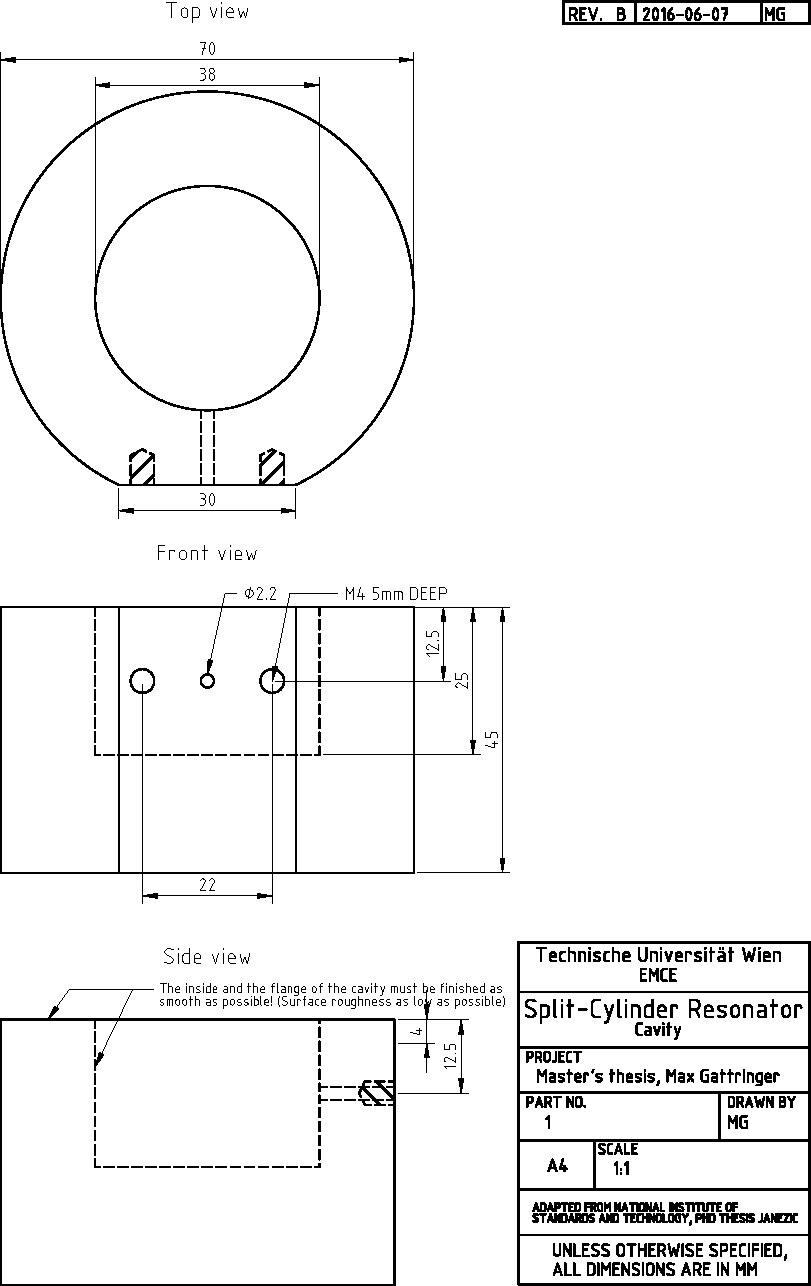
\includegraphics{Split_Cylinder_Drawing.pdf}
\caption{Drawing of the split-cylinder prototype, adapted from \cite{janezic}.}
\end{figure}
\end{appendices}
%%%%%%%%%% BILIOGRAPHY %%%%%%%%%%%%%%%%%
\bibliography{BIBLIOGRAPHY}
\addcontentsline{toc}{chapter}{Bibliography}
\newgeometry{total={13.5cm, 22cm}}
\chapter*{Declaration of Authorship}
\begin{otherlanguage}{german}
Hiermit erkläre ich, dass die vorliegende Arbeit gemäß dem Code of Conduct – Regeln zur Sicherung guter wissenschaftlicher Praxis (in der aktuellen Fassung des jeweiligen Mitteilungsblattes der TU Wien), insbesondere ohne unzulässige Hilfe Dritter und ohne Benutzung anderer als der angegebenen Hilfsmittel, angefertigt wurde. Die aus anderen Quellen direkt oder indirekt übernommenen Daten und Konzepte sind unter Angabe der Quelle gekennzeichnet. Die Arbeit wurde bisher weder im In– noch im Ausland in gleicher oder in ähnlicher Form in anderen Prüfungsverfahren vorgelegt.

\vspace{1cm}

\noindent Wien, am 20.04.2017

\noindent\includegraphics[height=1.7cm]{signature.png}
\end{otherlanguage}
\restoregeometry
\end{document}
